%
% Tutorial -- Modelling Operational Amplifiers
%
% Copyright (C) 2006 Mike Brinson <mbrin72043@yahoo.co.uk>
%
% Permission is granted to copy, distribute and/or modify this document
% under the terms of the GNU Free Documentation License, Version 1.1
% or any later version published by the Free Software Foundation.
%

% redefine subfigure caption
\renewcommand{\thesubfigure}{\thefigure(\alph{subfigure})}
\makeatletter
  \renewcommand{\@thesubfigure}{\thesubfigure:\space}
  \renewcommand{\p@subfigure}{}
\makeatother

% redefine subtable caption
\renewcommand{\thesubtable}{\thetable(\alph{subtable})}
\makeatletter
  \renewcommand{\@thesubtable}{\thesubtable:\space}
  \renewcommand{\p@subtable}{}
\makeatother

\tutsection{Introduction}

Operation amplifiers (OP AMP) are a fundamental building block of linear electronics.  They have been widely employed in linear circuit design since they were first introduced over thirty years ago. The use of operational amplifier models for circuit simulation using SPICE and other popular circuit simulators is widespread, and many manufacturers provide models for their devices. In most cases, these models do not attempt to simulate the internal circuitry at device level, but use macromodelling to represent amplifier behaviour as observed at the terminals of a device.  The purpose of this tutorial note is to explain how macromodels can be used to simulate a range of the operational amplifier properties and to show how macromodel parameters can be obtained from manufacturers data sheets.  This tutorial concentrates on models that can be simulated using Qucs release 0.0.9.




\tutsection{The Qucs built-in operational amplifier model}

Qucs includes a model for an ideal operational amplifier. It's symbol can be found in the nonlinear components list. This model represents an operational amplifier as an ideal device with differential gain and output voltage limiting. The model is intended for use as a simple gain block and should not be used in circuit simulations where operational amplifier properties are crucial to overall circuit performance. Fig.~\ref{fig:opamp1} shows a basic inverting amplifier with a gain of ten, based on the Qucs OP AMP model. The simulated AC performance of this circuit is shown in Fig.~\ref{fig:opamp2}.  From Fig.~\ref{fig:opamp2} it is observed that the circuit gain and phase shift are constant and do not change as the frequency of the input signal is increased. This, of course, is an ideal situation which practical operational amplifiers do not reproduce.  Let us compare the performance of the same circuit with the operational amplifier represented by a device level circuit. Shown in Fig.~\ref{fig:opamp3} is a transistor circuit diagram for the well known UA741 operational amplifier\footnote{The UA741 operational amplifier is one of the most studied devices. It is almost unique in that a transistor level model has been constructed for the device. Details of the circuit operation and modelling of this device can be found in (1) Paul R. Grey et. al., Analysis and Design of Analog Integrated Circuits, Fourth Edition, 2001, John Wiley and Sons INC., ISBN 0-471-32168-0, and (2) Andrei Vladimirescu, The SPICE book, 1994, John Wiley and Sons, ISBN 0-471-60926-9.}. The gain and phase results for the circuit shown in Fig.~\ref{fig:opamp1}, where the OP AMP is modelled by the UA741 transistor level model, are given in Fig.~\ref{fig:opamp4}.  The curves in this figure clearly illustrate the differences between the two simulation models.  When simulating circuits that include operational amplifiers the quality of the OP AMP model can often be a limiting factor in the accuracy of the overall simulation results.  Accurate OP AMP models normally include a range of the following device characteristics: (1) DC and AC differential gain, (2) input bias current, (3) input current and voltage offsets, (4) input impedance, (5) common mode effects, (6) slew rate effects, (7) output impedance, (8) power supply rejection effects, (9) noise, (10) output voltage limiting, (11) output  current limiting and (12) signal overload recovery effects. The exact mix of selected properties largely depends on the purpose for which the model is being used; for example, if a model is only required for small signal AC transfer function simulation then including the output voltage limiting section of an OP AMP model is not necessary or indeed may be considered inappropriate. In the following sections of this tutorial article macromodels for a number of the OP AMP parameters listed above are developed and in each case the necessary techniques are outlined showing how to derive macromodel parameters from manufacturers data sheets.


\begin{figure}
  \centering
  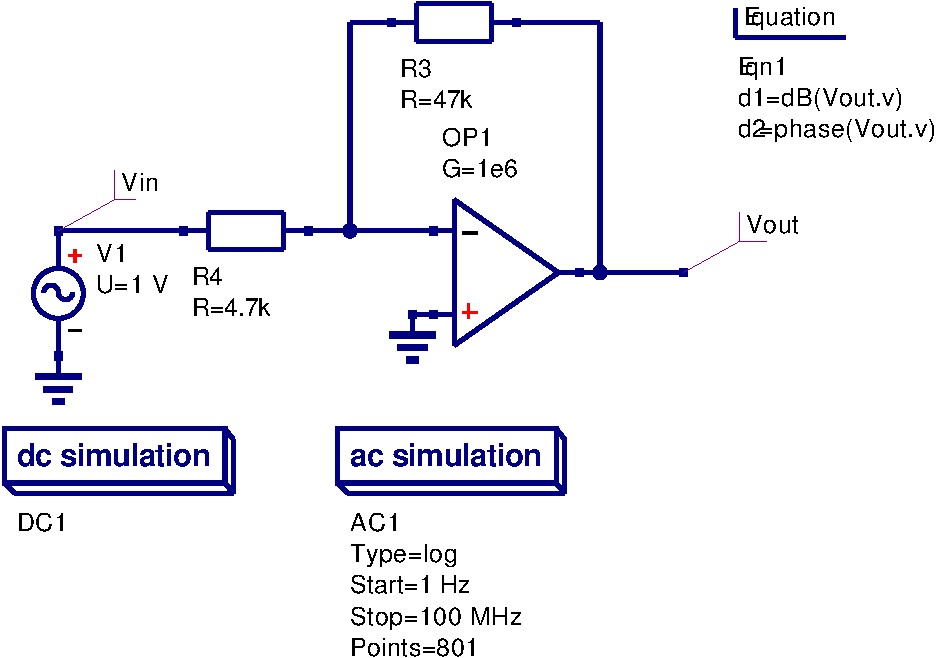
\includegraphics[width=0.9\linewidth]{fig1_sch}
  \caption{Qucs schematic for a basic OP AMP inverting amplifier:Qucs OP AMP has G=1e6 and Umax=15V.}
  \label{fig:opamp1}
\end{figure} 

\begin{figure}
  \centering
  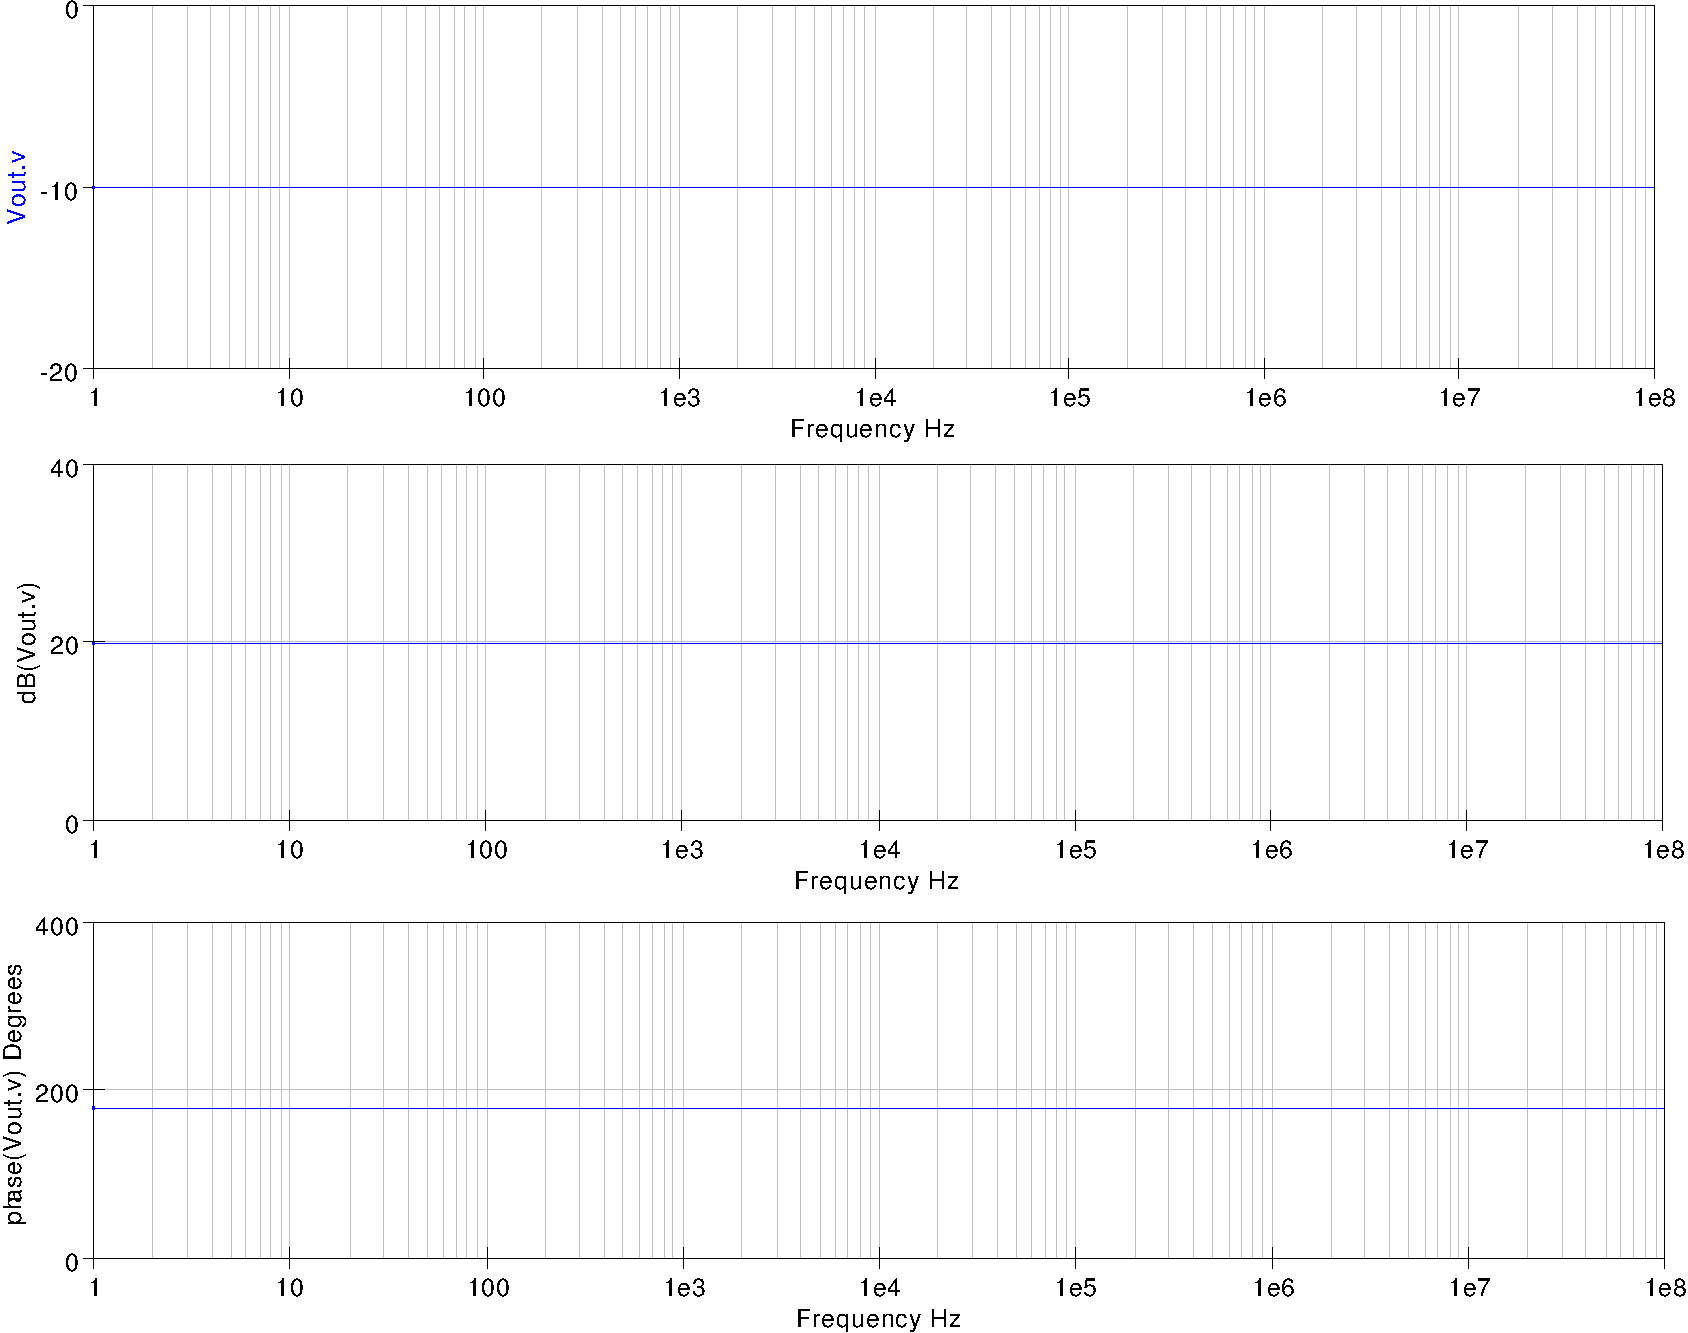
\includegraphics[width=0.9\linewidth]{fig1_dpl}
  \caption{Gain and phase curves for a basic OP AMP inverting amplifier.}
  \label{fig:opamp2}
\end{figure} 

\begin{figure}
  \centering
  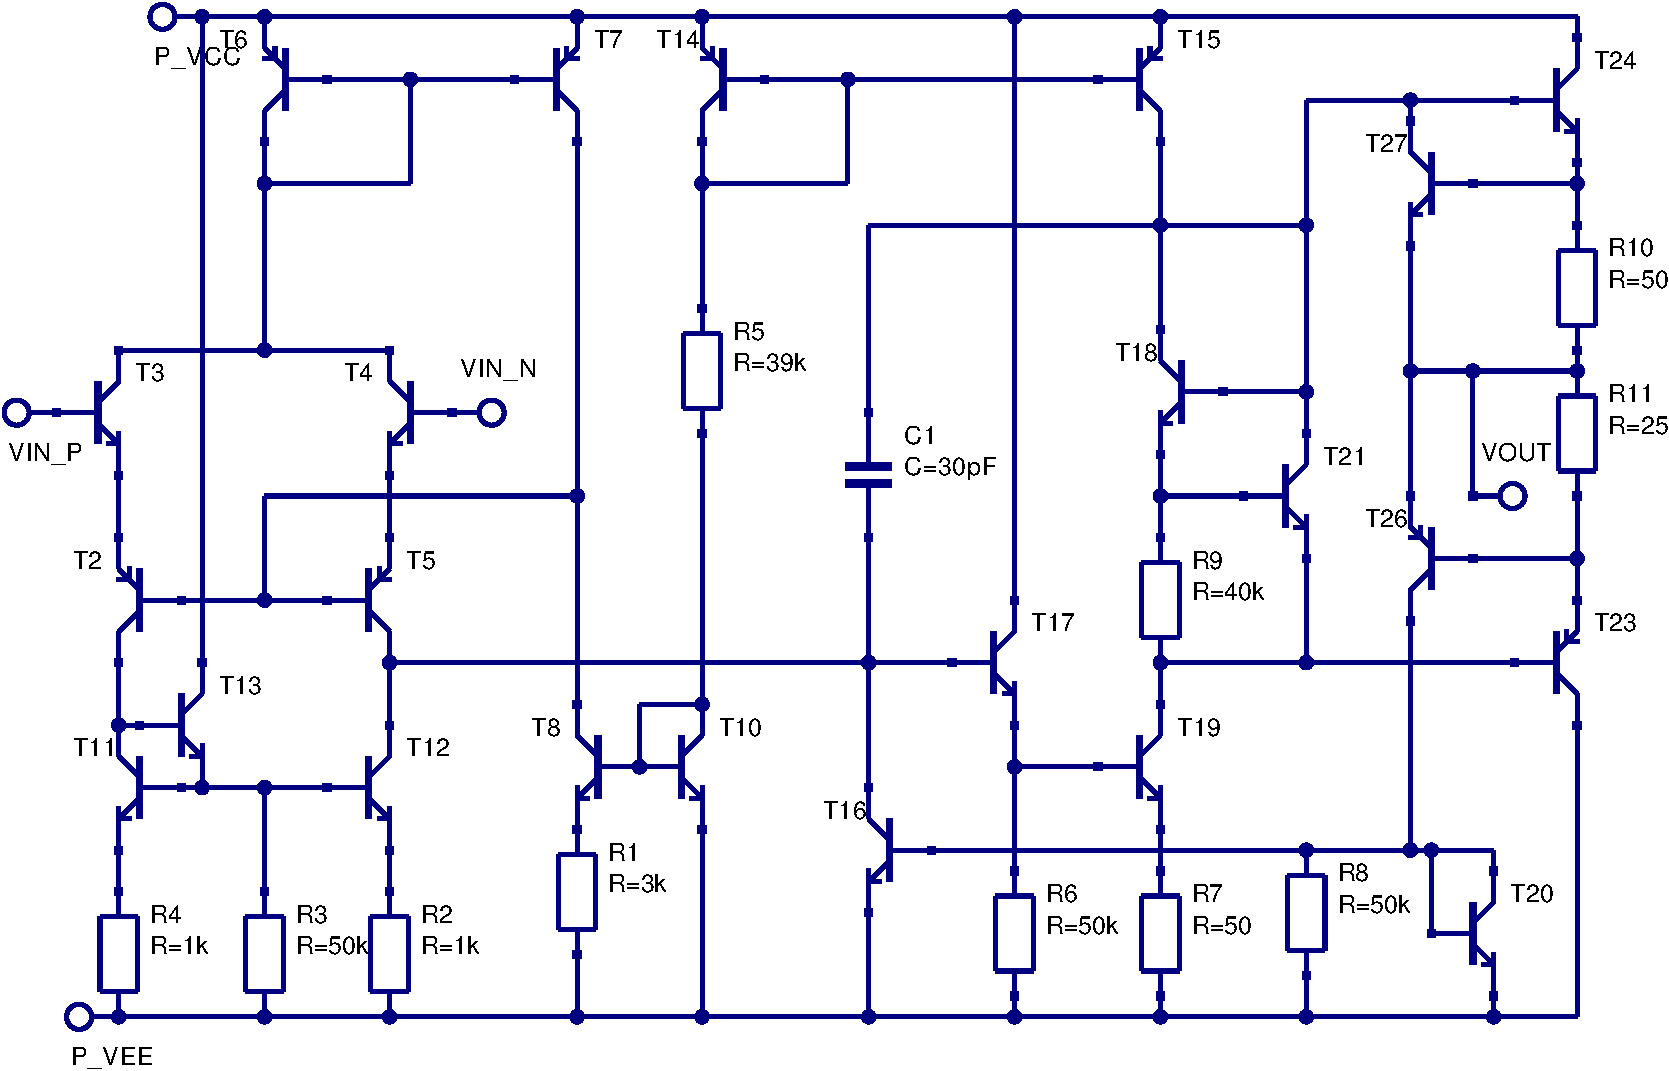
\includegraphics[width=0.9\linewidth]{fig2_sch}
  \caption{Transistor level circuit for the UA741 operational amplifier.}
  \label{fig:opamp3}
\end{figure} 


\begin{figure}
  \centering
  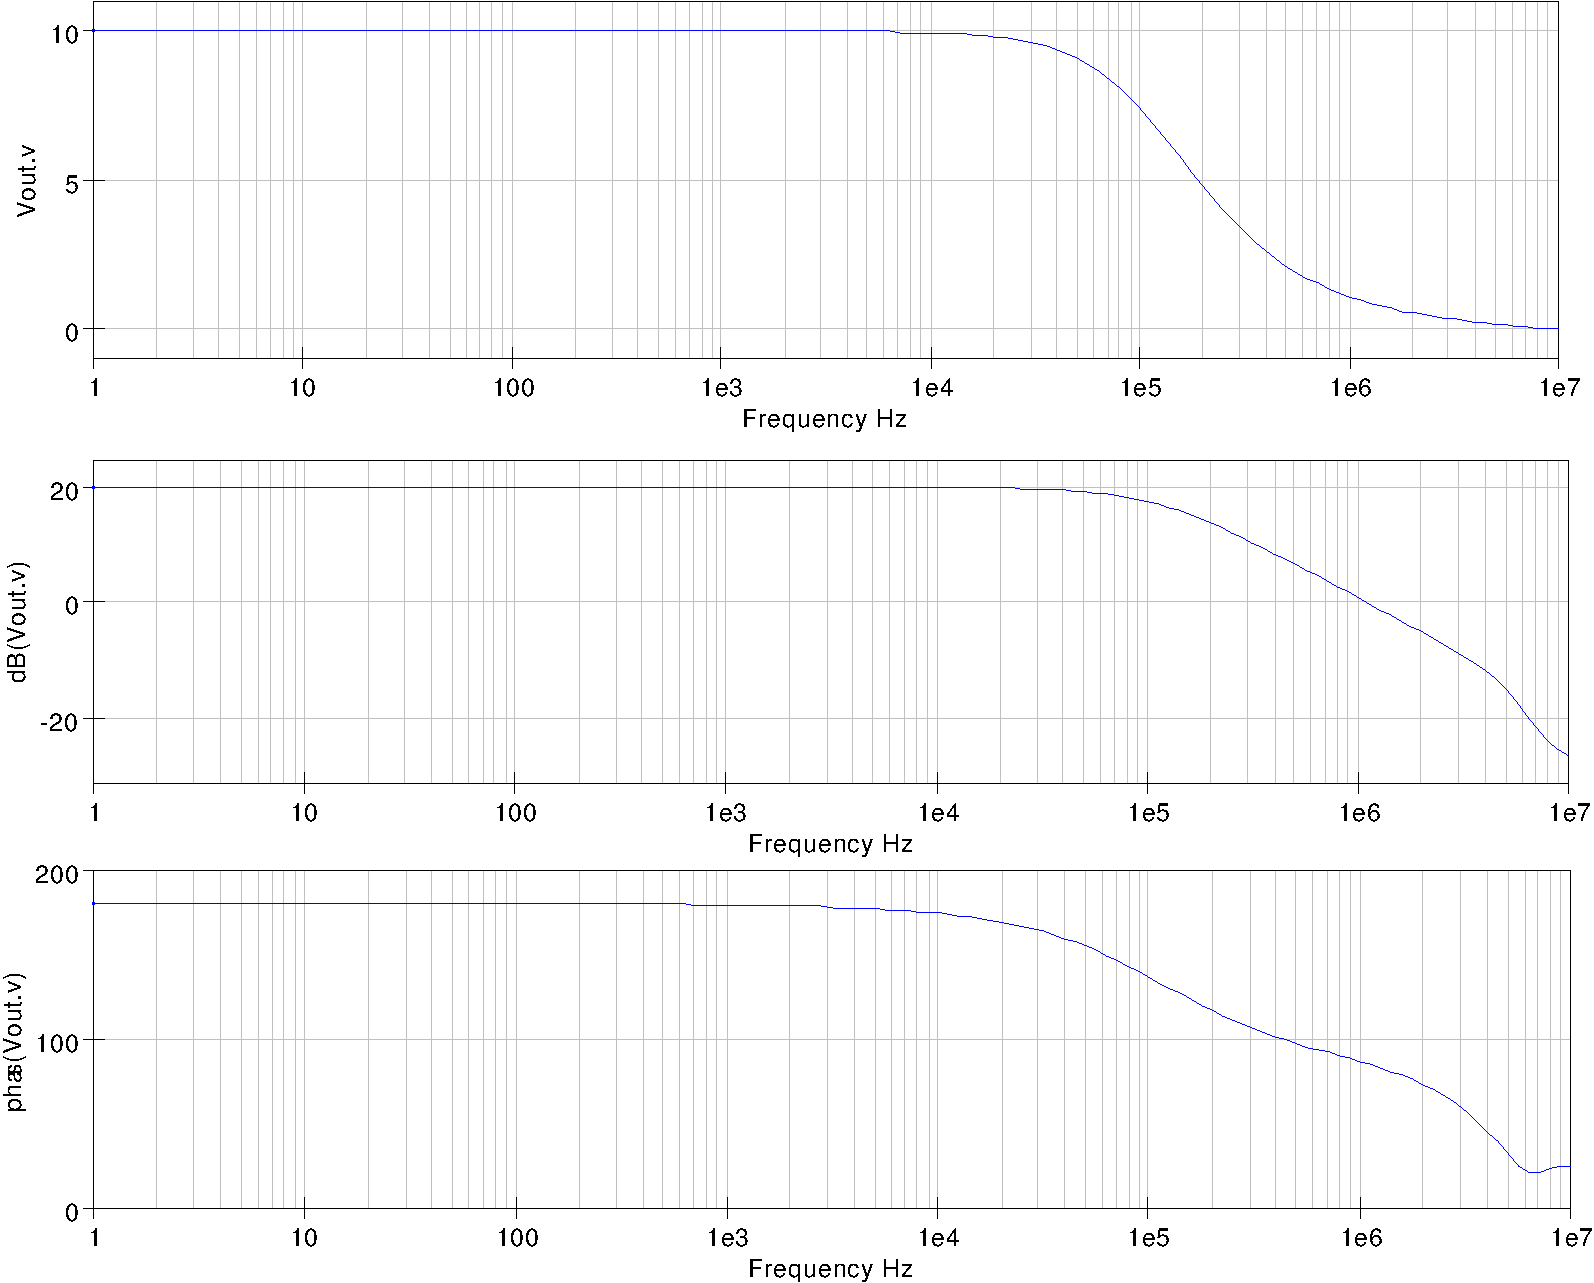
\includegraphics[width=0.9\linewidth]{fig2_dpl}
  \caption{Gain and phase curves for a times 10 inverting amplifier with the OP AMP represented by a transistor level UA741 model.}
  \label{fig:opamp4}
\end{figure} 


\begin{figure}
  \centering
  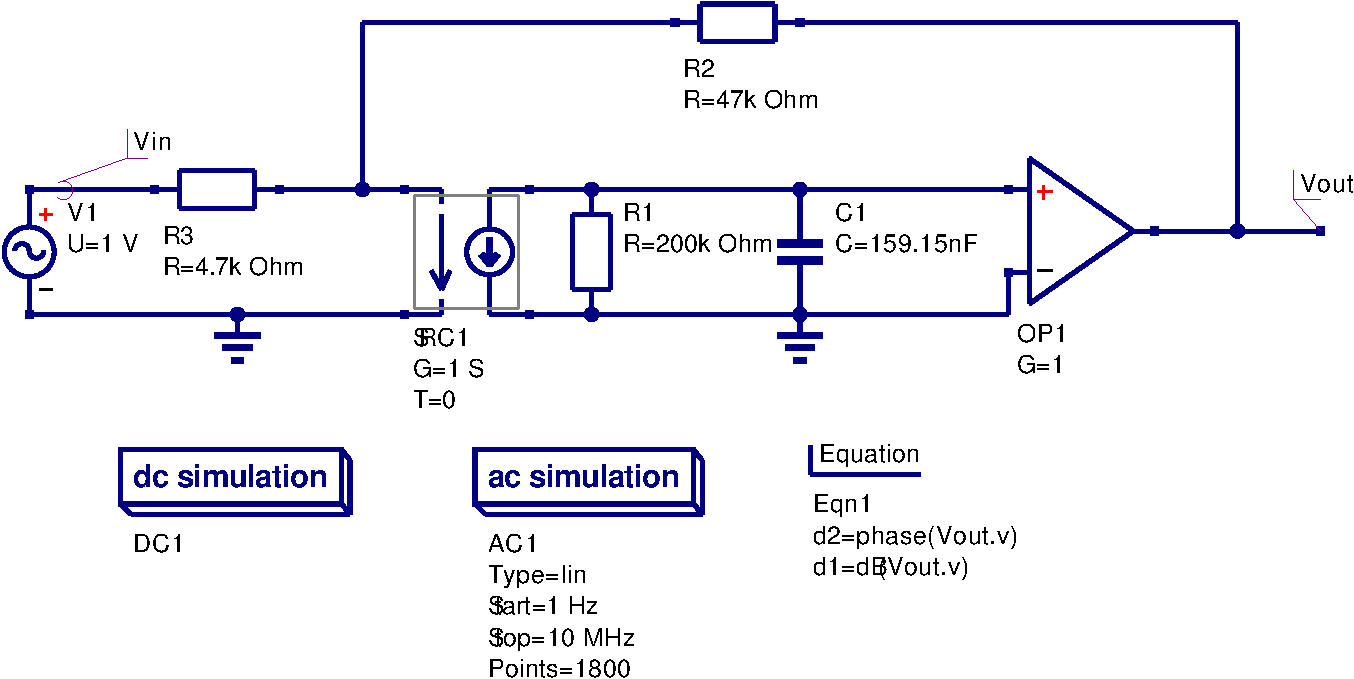
\includegraphics[width=0.9\linewidth]{fig3_sch}
  \caption{Modified Qucs OP AMP model to include single pole frequency response.}
  \label{fig:opamp5}
\end{figure} 

\begin{figure}
  \centering
  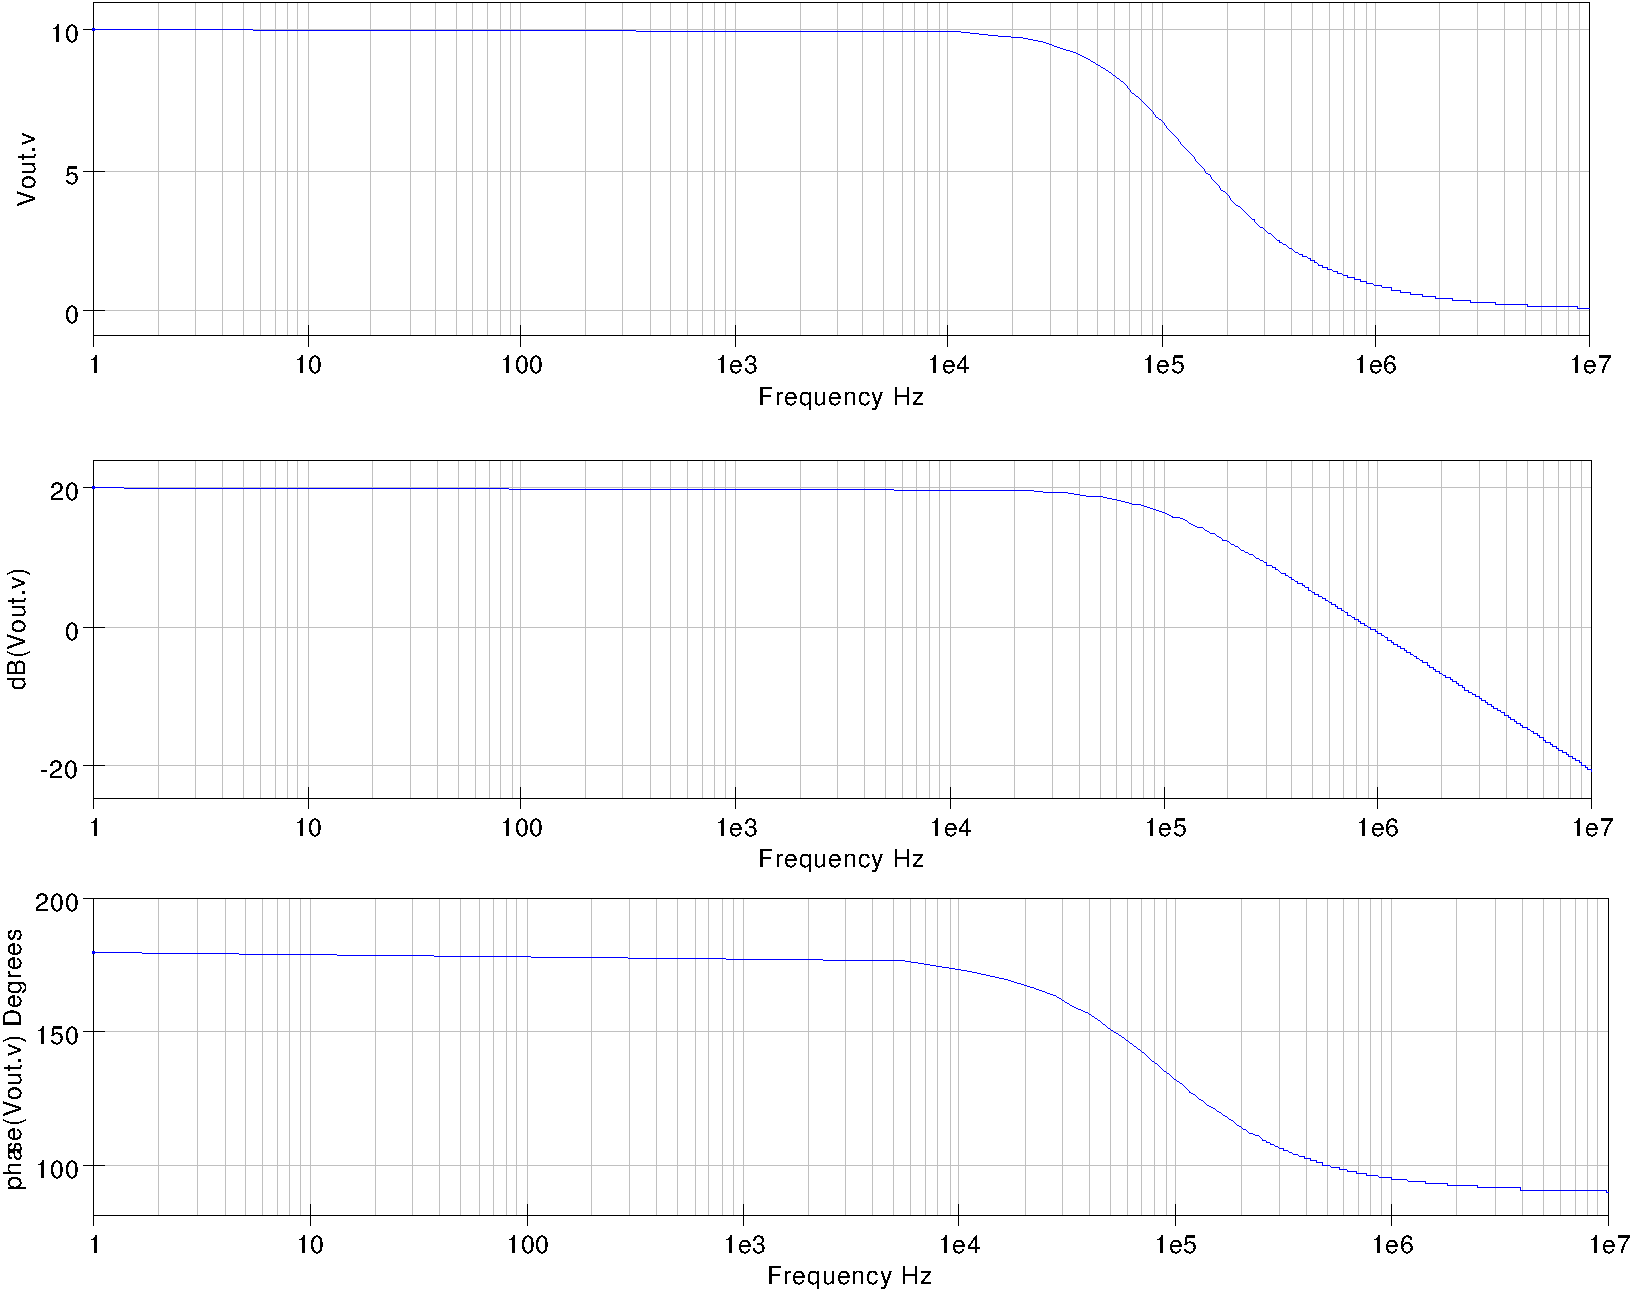
\includegraphics[width=0.9\linewidth]{fig3_dpl}
  \caption{Gain and phase curves for the circuit shown in Fig.~\ref{fig:opamp5}.}
  \label{fig:opamp6}
\end{figure} 

\tutsection{Adding features to the Qucs OP AMP model}

In the previous section it was shown that the Qucs OP AMP model had a frequency response that is independent of frequency.  By adding external components to the Qucs OP AMP model the functionality of the model can be improved.  The UA741 differential open loop gain has a pole at roughly 5Hz and a frequency response that decreases at 20 dB per frequency decade from the first pole frequency up to a second pole frequency at roughly 3 MHz. The circuit shown in Fig.~\ref{fig:opamp5} models the differential frequency characteristics of a UA741 from DC to around 1 MHz. Figure ~\ref{fig:opamp6} illustrates the closed loop frequency response for the modified Qucs OP AMP model.



\tutsection{Modular operational amplifier macromodels}

Macromodelling is a term given to the process of modelling an electronic device as a "black box" where individual device characteristics are specified in terms of the signals, and other properties, observed at the input and output terminals of the black box.  Such models operate at a functional level rather than at the more detailed transistor circuit level, offering considerable gain in computational efficiency.\footnote{  Computational efficiency is increased mainly due to the fact that operational amplifier macromodels have, on average, about one sixth of the number of nodes and branches when compared to a transistor level model.  Furthermore, the number of non-linear p-n junctions included in  a macromodel is often less than ten which compares favorable with the forty to fifty needed to model an amplifier at transistor level.}  Macromodels are normally derived directly from manufacturers data sheets.  For the majority of operational amplifiers, transistor level models are not normally provided by manufacturers.  One notable exception being the UA741 operational amplifier shown in Fig.~\ref{fig:opamp3}.\\
A block diagram of a modular\footnote{Brinson M. E. and Faulkner D. J., Modular SPICE macromodel for operational amplifiers, IEE Proc.-Circuits Devices Syst., Vol. 141, No. 5, October 1994, pp. 417-420.} general purpose OP AMP macromodel is illustrated in Fig.~\ref{fig:opamp7}.  In this diagram the blocks represent specific amplifier characteristics modelled by electrical networks composed of components found in all the popular circuit simulators\footnote{Models employing non-linear controlled sources, for example the SPICE B voltage and current sources, are not allowed in Qucs release 0.0.9. Non-linear controlled sources are one of the features on the Qucs to-do list.}. Each block consists of one or more components which model a single amplifier parameter or a group of related parameters such as the input offset current and voltage.  This ensures that changes to one particular parameter do not indirectly change other parameters.  Local nodes and scaling are also employed in the macromodel blocks.  Furthermore, because each block operates separately, scaled voltages do not propagate outside individual blocks. Each block can be modelled with a Qucs subcircuit that has the required specification and buffering from other blocks.  Moreover, all subcircuits are self contained entities where the internal circuit details are hidden from other blocks.  Such an approach is similar to structured high-level computer programming where the internal details of functions are hidden from users.   Since the device characteristics specified by each block are separate from all other device characteristics only those amplifier characteristics which are needed are included in a given macromodel. This approach leads to a genuinely structured macromodel.  The following sections present the detail and derivation of the electrical networks forming the blocks drawn in Fig.~\ref{fig:opamp7}. To illustrate the operation of the modular OP AMP macromodel the values of the block parameters are calculated for the UA741 OP AMP and used in a series of example simulations.  Towards the end of this tutorial note data are presented for a number of other popular general purpose operational amplifiers.
\tutsection{A basic AC OP AMP macromodel. }

A minimum set of blocks is required for the modular macromodel to function as an amplifier: an input stage, a gain stage and an output stage.  These form the core modules of all macromodels.  

\tutsubsection{The input stage.}
The input stage includes amplifier offset voltage, bias and offset currents, and the differential input impedance components. The circuit for the input stage is shown in Fig.~\ref{fig:opamp8}, where
\begin{enumerate}
\item \textit{R1   = R2} = Half of the amplifier differential input resistance (\textit{RD}).
\item \textit{Cin}   = The amplifier differential input capacitance (\textit{CD}).
\item \textit{Ib1    = Ib2} = The amplifier input bias current (\textit{IB}).
\item \textit{Ioff}  = Half the amplifier input offset current (\textit{IOFF}).
\item \textit{Voff1 = Voff2} = Half the input offset voltage ( \textit{VOFF}).
\end{enumerate}

Typical values for the UA741 OP AMP are:

\begin{enumerate}
\item \textit{RD} = 2 M$\Omega$ and \textit{R1 = R2} = 1M$\Omega$
\item \textit{CD} = \textit{Cin1} = 1.4 pF.
\item \textit{IB} = \textit{Ib1} = \textit{Ib2 }= 80 nA.
\item \textit{IOFF} = 20 nA and \textit{Ioff1} = 10 nA.
\item \textit{VOFF} = 0.7 mV and \textit{Voff1 = Voff2} = 0.35 mV.
\end{enumerate}

\FloatBarrier
\begin{figure}
  \centering
  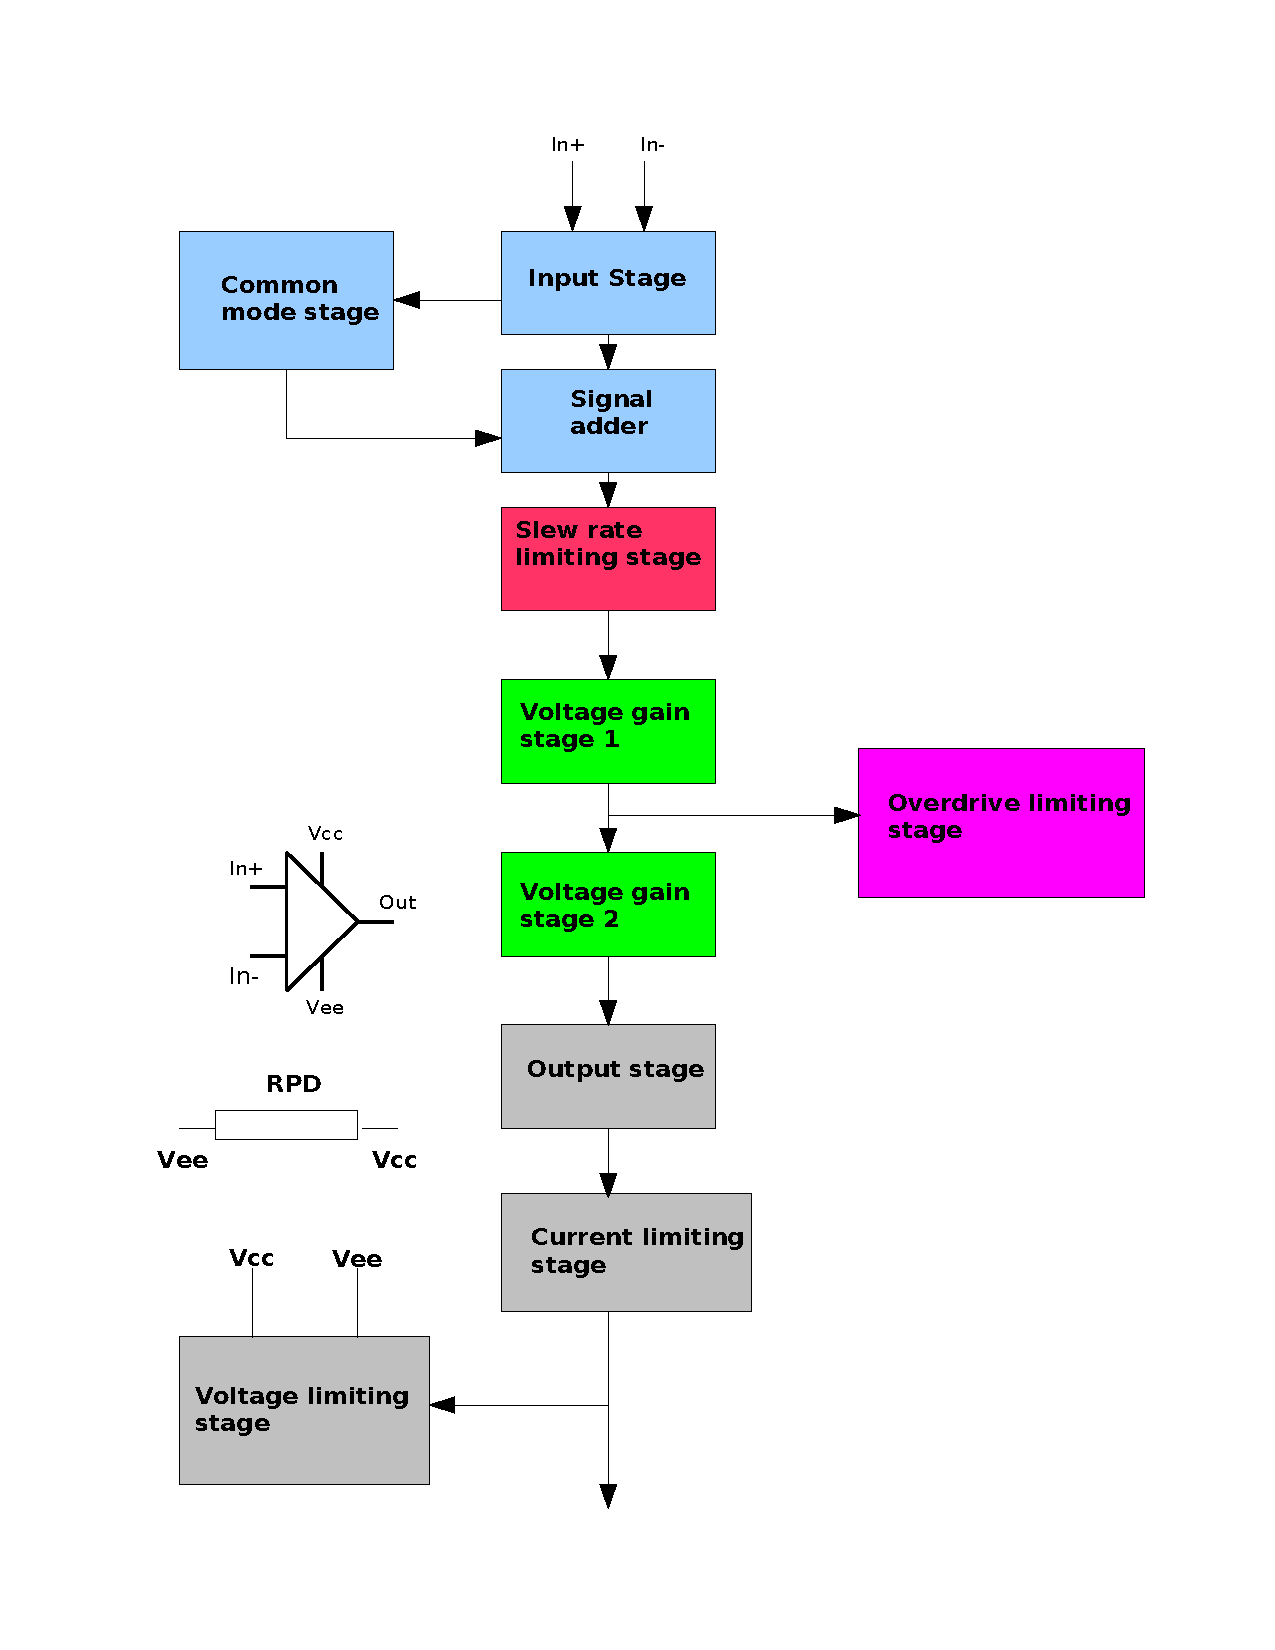
\includegraphics[width=1.0\linewidth]{dwr1}
  \caption{Block diagram of an operational amplifier macromodel.} 
  \label{fig:opamp7}
\end{figure} 
\FloatBarrier


The differential output signal (VD) is given by $VD_{-}P1 - VD_{-}N1$ and the common mode output signal (\textit{VCM}) by $(VD_{-}P1 + VD_{-}N1)/2$.
\FloatBarrier
\begin{figure}
  \centering
  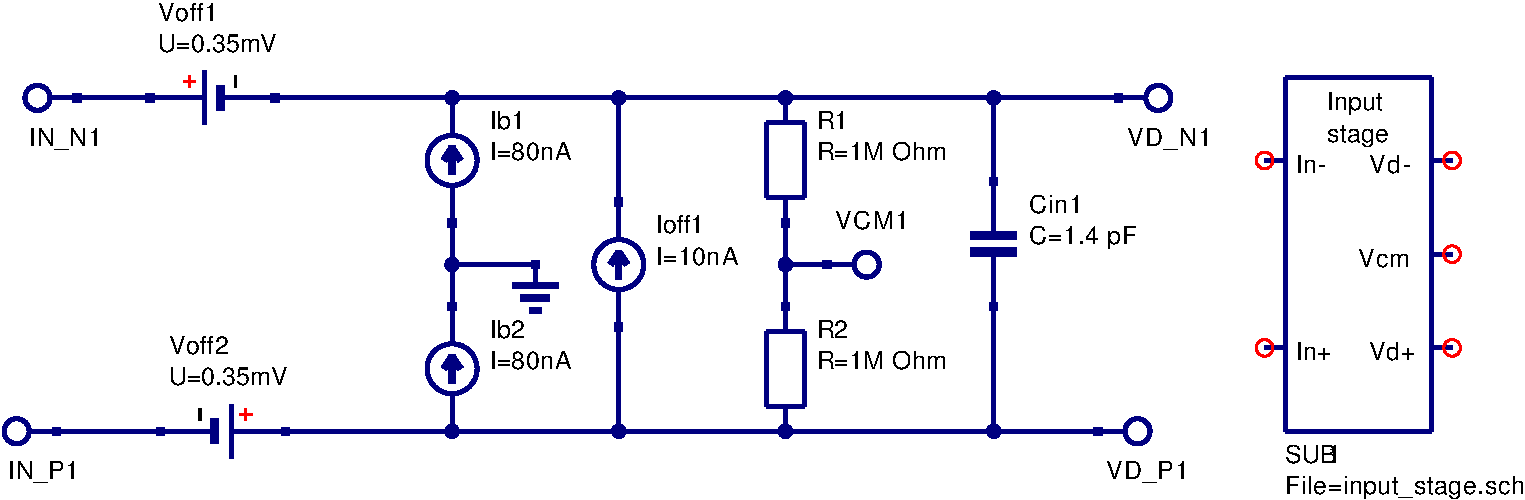
\includegraphics[width=1.0\linewidth]{fig8_sch}
% tcomb1.png: 99.9998dpi, width=11.35cm, height=3.35cm, bb=0 0 447 132
  \caption{Modular OP AMP input stage block.}
  \label{fig:opamp8}
\end{figure}
\FloatBarrier

\tutsubsection{Voltage gain stage 1.}
The circuit for voltage gain stage 1 is shown in Fig.~\ref{fig:opamp9}, where
\begin{enumerate}
\item\textit{ RD1} = 100 M$\Omega$ = A dummy input resistor - added to ensure nodes $IN_{-}P1$ and $IN_{-}N1$ are connected by a DC path.
\item \textit{GMP1} = 1 S = Unity gain voltage controlled current generator.
\item \textit{RADO }= The DC open loop differential gain ( \textit{AOL(DC)} ) of the OP AMP.
\item \textit{CP1}  = \textit{1/(2*$\pi$*GBP)}, where \textit{GBP} = the OP AMP gain bandwidth product.
\end{enumerate}

Typical values for the UA741 OP AMP are:
\begin{enumerate}
\item \textit{RADO} =  200k$\Omega$. ($AOL(DC)$ = 106 dB)
\item \textit{CP1}  =  159.15 nF  (The typical value for UA741 GBP is 1 MHz).
\end{enumerate}



\FloatBarrier
\begin{figure}
  \centering
  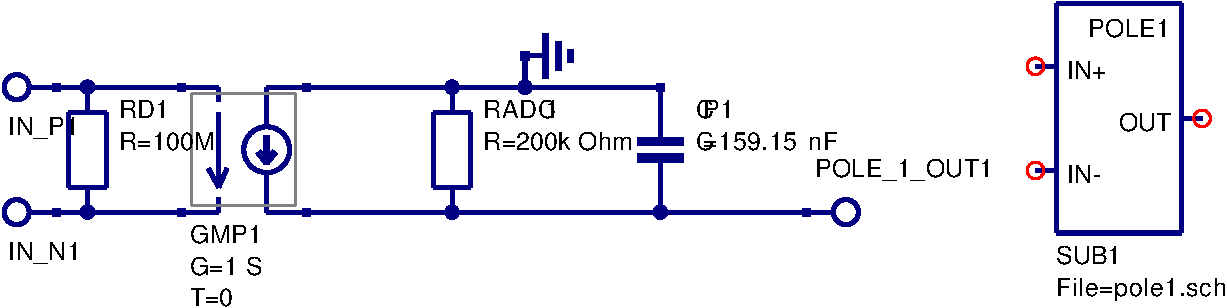
\includegraphics[width=1.0\linewidth]{fig9_sch}
% tcomb1.png: 99.9998dpi, width=11.35cm, height=3.35cm, bb=0 0 447 132
  \caption{Modular OP AMP first voltage gain stage.}
  \label{fig:opamp9}
\end{figure}



\tutsubsection{Derivation of voltage gain stage 1 transfer function.}

Most general purpose operational amplifiers have an open loop differential voltage gain which has (1) a very high value at DC (2) a dominant pole (\textit{fp1}) at a low frequency - typically below 100 Hz, and (3) a gain response characteristic that rolls-off at 20 dB per decade up to a unity gain frequency which is often in the MHz region.  This form of response has a constant gain bandwidth product (\textit{GBP}) over the frequency range from \textit{fp1} to \textit{GBP}.  A typical OP AMP differential open loop response is shown in Fig.~\ref{fig:opamp10}. The voltage gain transfer function for this type of characteristic can be modelled with the electrical network given in Fig.~\ref{fig:opamp9}, where the the AC voltage transfer function is


\begin{equation}
vout(POLE_{-}1_{-}OUT1) = \dfrac{ GMP1 * ( V( IN _{-} P1 ) - V(IN _{-} N1) ) * RADO} { 1 + j (\omega * RADO * CP1 ) }
\end{equation}
Where \begin{equation}
        f_{P1} = \dfrac {1} {2\pi * RADO * CP1}
      \end{equation}
Let \textit{RADC = Aol(DC)} and \textit{GMP1 = 1 S}. Then, because \textit{fp1*AOL(DC) = GBP},
\begin{equation} 
CP1 = \dfrac{1} { 2\pi*GBP}
\end{equation}

\begin{figure}
  \centering
  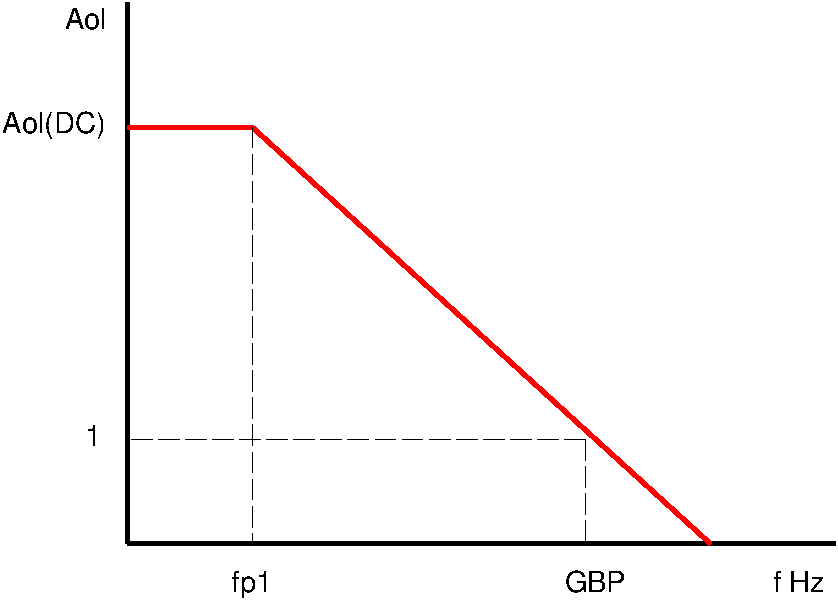
\includegraphics[width=0.8\linewidth]{fig10_diag}
% tcomb1.png: 99.9998dpi, width=11.35cm, height=3.35cm, bb=0 0 447 132
  \caption{OP AMP open loop differential voltage gain as a function of frequency.}
  \label{fig:opamp10}
\end{figure}

\newpage 

\tutsubsection{Output stage.}
The electrical network representing a basic output stage is given in Fig.~\ref{fig:opamp11}, where

\begin{enumerate}
\item \textit{ RD1}     = 100 M$\Omega$ = A dummy input resistor - added to ensure nodes $IN_{-}P1$ and $IN_{-}N1$ are connected by a DC path.
\item \textit{EOS1}   G = 1 = Unity gain voltage controlled voltage generator.
\item \textit{ROS1}     =  OP AMP output resistance.
\end{enumerate}

A typical value for the UA741 OP AMP output resistance is \textit{ROS1} =  75$\Omega$.


\begin{figure}
  \centering
  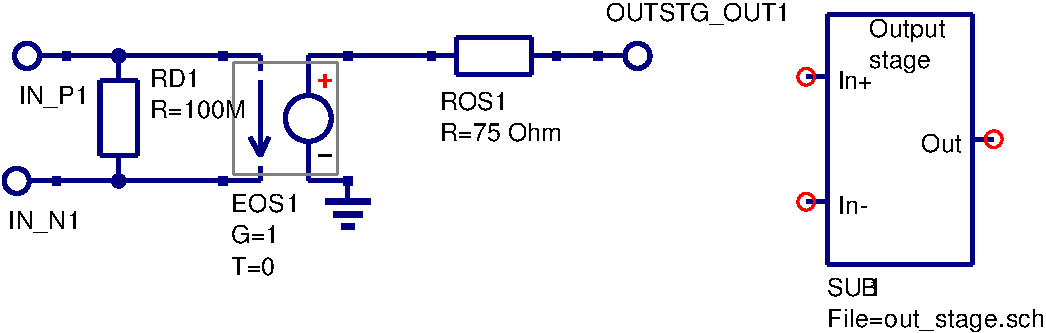
\includegraphics[width=0.8\linewidth]{fig11_sch}
% tcomb1.png: 99.9998dpi, width=11.35cm, height=3.35cm, bb=0 0 447 132
  \caption{Modular macromodel output stage.}
  \label{fig:opamp11}
\end{figure}

\tutsubsection{A subcircuit model for the basic AC OP AMP macromodel.}
The model for the basic AC OP AMP macromodel is shown in Fig.~\ref{fig:opamp12}. The input stage common mode voltage ($Vcm$) is not used in this macromodel and has been left floating.  To test the performance of the AC macromodel it's operation was compared to the transistor level UA741 model. Figure ~\ref{fig:opamp13} shows a schematic circuit for two inverting amplifiers, each with a gain of ten, driven from a common AC source. One of the amplifiers uses the simple AC macromodel and the other the transistor level UA741 model.  Figure ~\ref{fig:opamp14} illustrates the output gain and phase curves for both amplifiers. In general the plotted curves are very similar.  However, at frequencies above the GBP frequency the basic AC macromodel does not correctly model actual OP AMP performance. This is to be expected because the simple AC macromodel does not include any high frequency modelling components.  Notice also that the DC output voltages for vout and vout3 are very similar, see the DC tabular results given in Fig.~\ref{fig:opamp13}. 

\begin{figure}
  \centering
  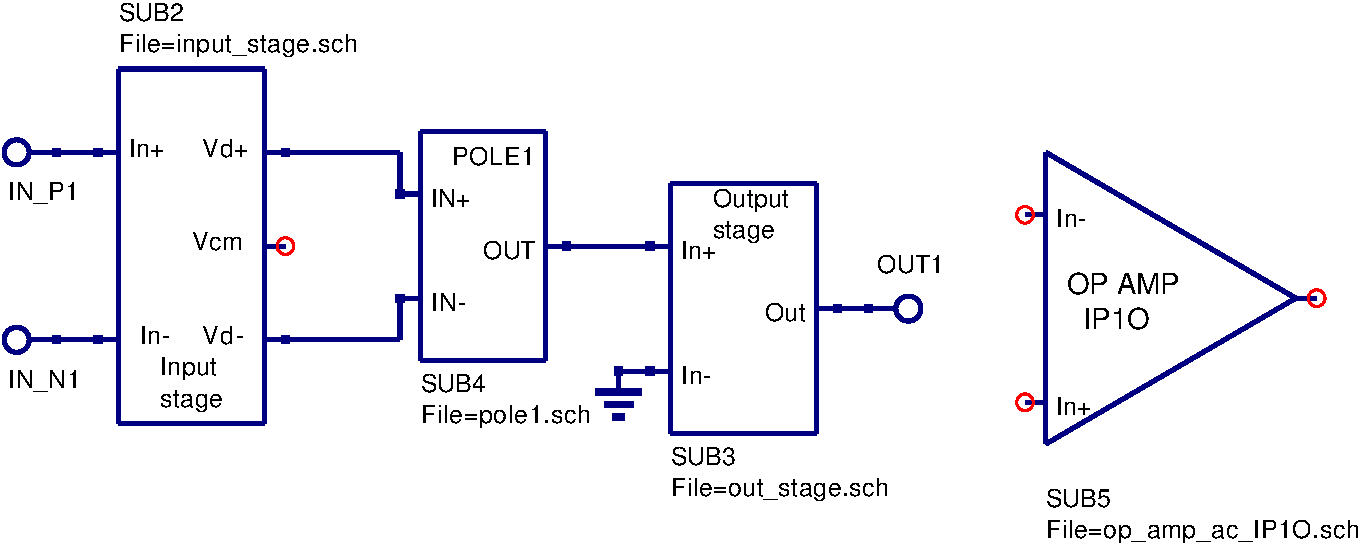
\includegraphics[width=1.0\linewidth]{fig12_sch} 
% tcomb1.png: 99.9998dpi, width=11.35cm, height=3.35cm, bb=0 0 447 132 
  \caption{Simple AC OP AMP macromodel.}
  \label{fig:opamp12}
\end{figure}

\begin{figure}
  \centering
  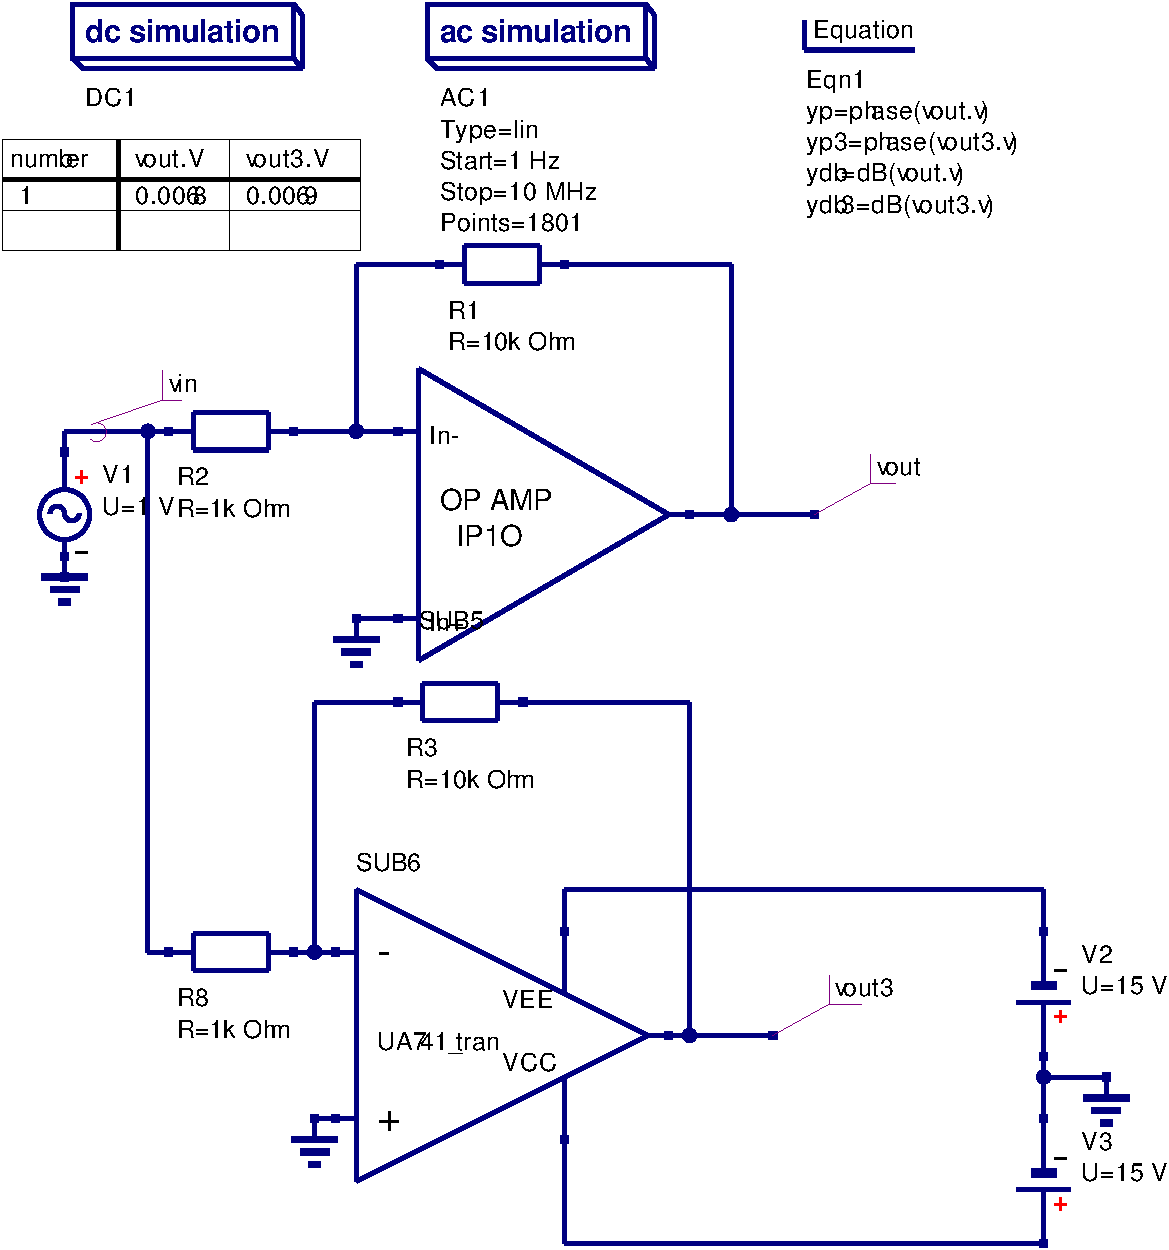
\includegraphics[width=0.9\linewidth]{fig13_sch}
% tcomb1.png: 99.9998dpi, width=11.35cm, height=3.35cm, bb=0 0 447 132
 \caption{Test circuit for an inverting amplifier. Output signals: (1) vout for AC macromodel, (2) vout3 for UA741 transistor model.}
  \label{fig:opamp13}
\end{figure}

\begin{figure}
  \centering
  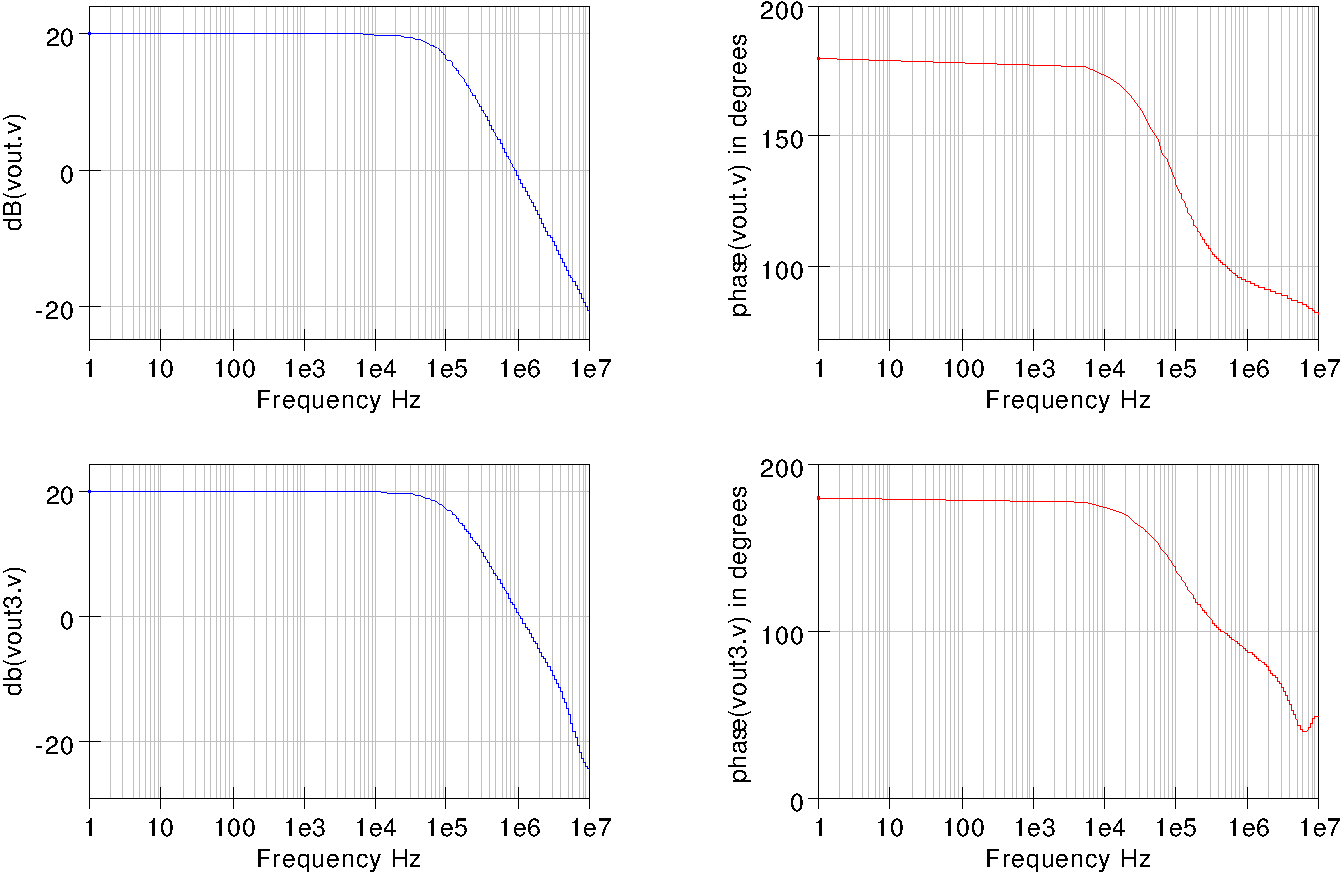
\includegraphics[width=0.9\linewidth]{fig14_dpl}
% tcomb1.png: 99.9998dpi, width=11.35cm, height=3.35cm, bb=0 0 447 132
  \caption{Simulation test results for the circuit shown in Fig.~\ref{fig:opamp13}.} 
  \label{fig:opamp14}
\end{figure}

\tutsection{ A more accurate OP AMP AC macromodel}

Most general purpose OP AMPs have a high frequency pole in their differential open loop gain characteristics.  By adding a second gain stage to the simple AC macromodel the discrepancy in the high frequency response can be corrected.  The model for the second gain stage is shown in Fig.~\ref{fig:opamp15}.  This additional gain stage has a structure similar to the first gain stage, where

\begin{enumerate}
\item\textit{RD2} = 100 M$\Omega$ = A dummy input resistor - added to ensure nodes \verb|IN_P2| and \verb|IN_N2| are connected by a DC path.
\item \textit{GMP2} = 1 S = Unity gain voltage controlled current generator.
\item \textit{RP2 } = 1$\Omega$.
\item \textit{CP2}  = \textit{1/(2$\pi$*fp2)}, where $fp2$ = the second pole frequency in Hz.
\end{enumerate}

A typical value for the UA741 OP AMP high frequency pole is  \textit{fp2}  =  3M Hz 


\begin{figure}
  \centering
  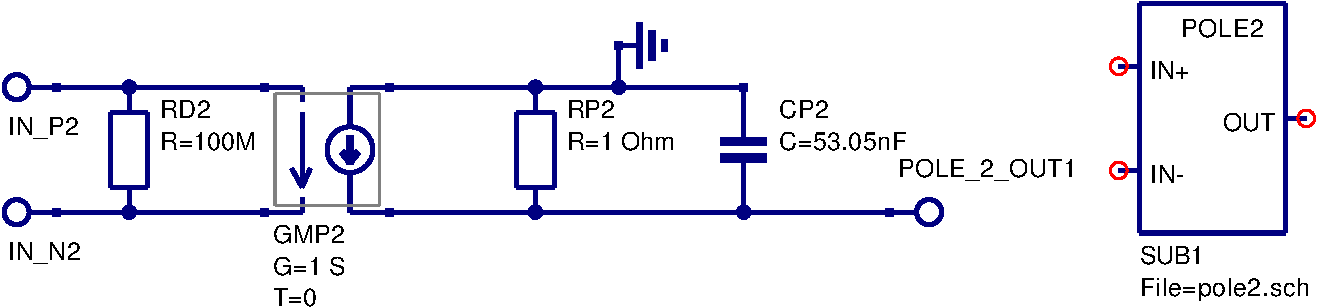
\includegraphics[width=0.9\linewidth]{fig15_sch}
% tcomb1.png: 99.9998dpi, width=11.35cm, height=3.35cm, bb=0 0 447 132
  \caption{Modular OP AMP second voltage gain stage.}
  \label{fig:opamp15}
\end{figure}

\tutsubsection{Derivation of voltage gain stage 2 transfer function.}
The differential voltage gain transfer function for voltage gain stage 2 is given by

\begin{equation}
vout(POLE_{-}2_{-}OUT1) = \dfrac{ GMP2 * ( V( IN _{-} P2 ) - V(IN _{-} N2) ) * RP2} { 1 + j (\omega * RP2 * CP2 ) }
\end{equation}

Let \textit{RP2 = 1$\Omega$} and \textit{GMP2 = 1 S}. Then 

\begin{equation}
vout(POLE_{-}2_{-}OUT1) = \dfrac{ V( IN _{-} P2 ) - V(IN _{-} N2)} { 1 + j (\omega *  CP2 ) }
\end{equation}

and

\begin{equation} 
CP2 = \dfrac{1} { 2\pi*fp2}
\end{equation}

\newpage
\tutsubsection{Simulating OP AMP open loop differential gain.}

The circuit shown in Fig.~\ref{fig:opamp16} allows the open loop differential gain \textit{(Aol(f))} to be simulated. This circuit employes a feedback resistor to ensure DC stability.  Fig.~\ref{fig:opamp16} illustrates two test circuits driven from a common AC source. This allows the performance of the AC macromodel and the UA741 transistor level model to be compared. The AC voltage transfer function for the test circuit is
  
\begin{equation}
vout(f) = \dfrac{ Aol(f)} { 1 +  \dfrac{ Aol(f) }{1 + j \omega * R * C} } vin(f)
\end{equation} 

where $vout(f) = (V^{+} - V^{-})*Aol(f)$,  $V^{+} = vin(f)$, and $V^{-} = \dfrac{vout(f)}{1 + j \omega * R * C} $

Provided $\dfrac{Aol(f)}{\omega*R*C} << 1$, equation (7) becomes $vout(f) \Rightarrow Aol(f) * vin(f)$. Hence, for those frequencies where this condition applies \textit{vout(f) = Aol(f)} when\textit{ vin(f)} = 1 V.  Figure 17 shows plots of the open loop simulation data. Clearly with the test circuit time constant set at 1e6 seconds the data is accurate for frequencies down to 1 Hz. 


\begin{figure}
  \centering
  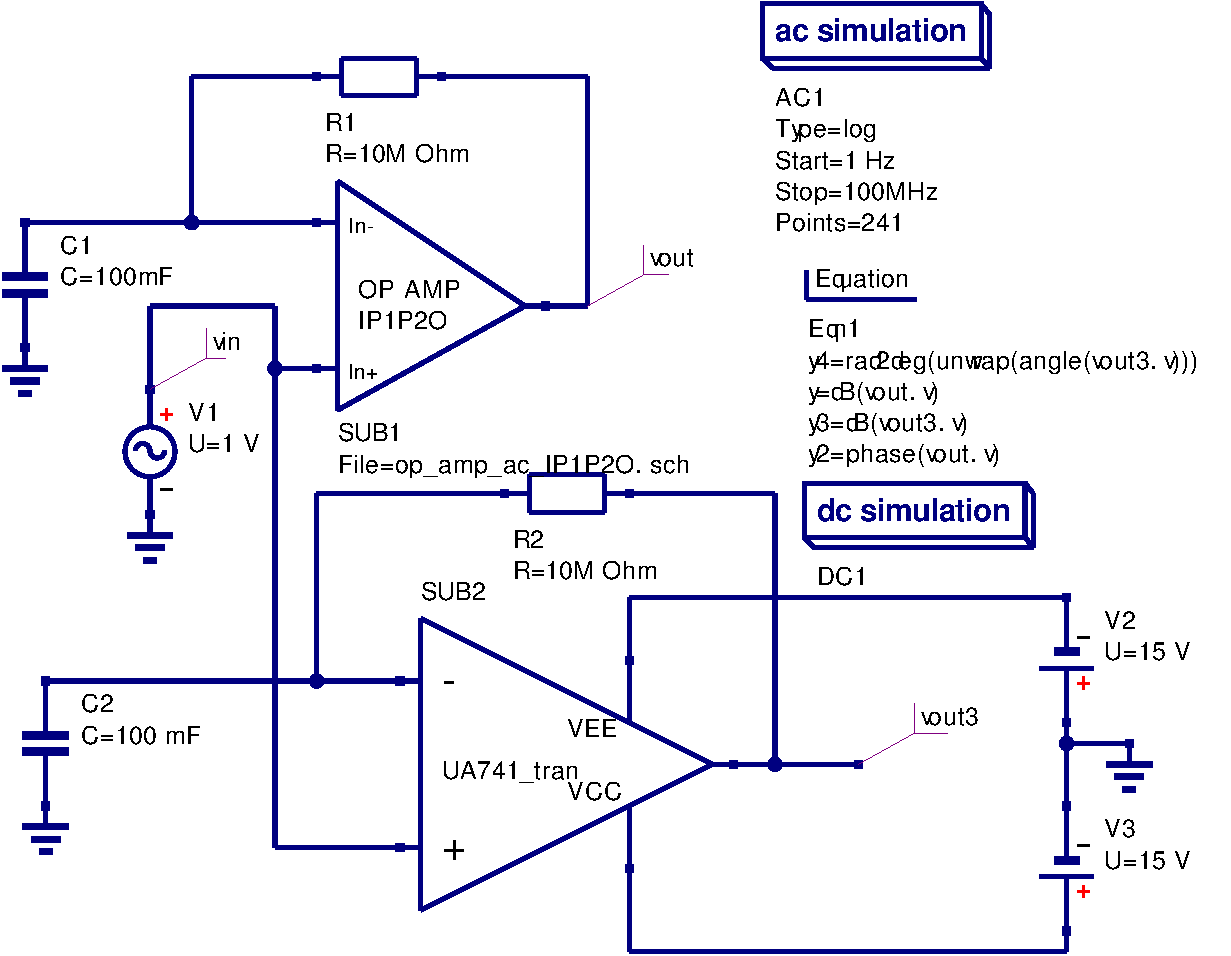
\includegraphics[width=0.8\linewidth]{fig16_sch}
% tcomb1.png: 99.9998dpi, width=11.35cm, height=3.35cm, bb=0 0 447 132
  \caption{Test circuit for simulating OP AMP open loop differential gain.}  
  \label{fig:opamp16}
\end{figure}

\begin{figure}
  \centering
  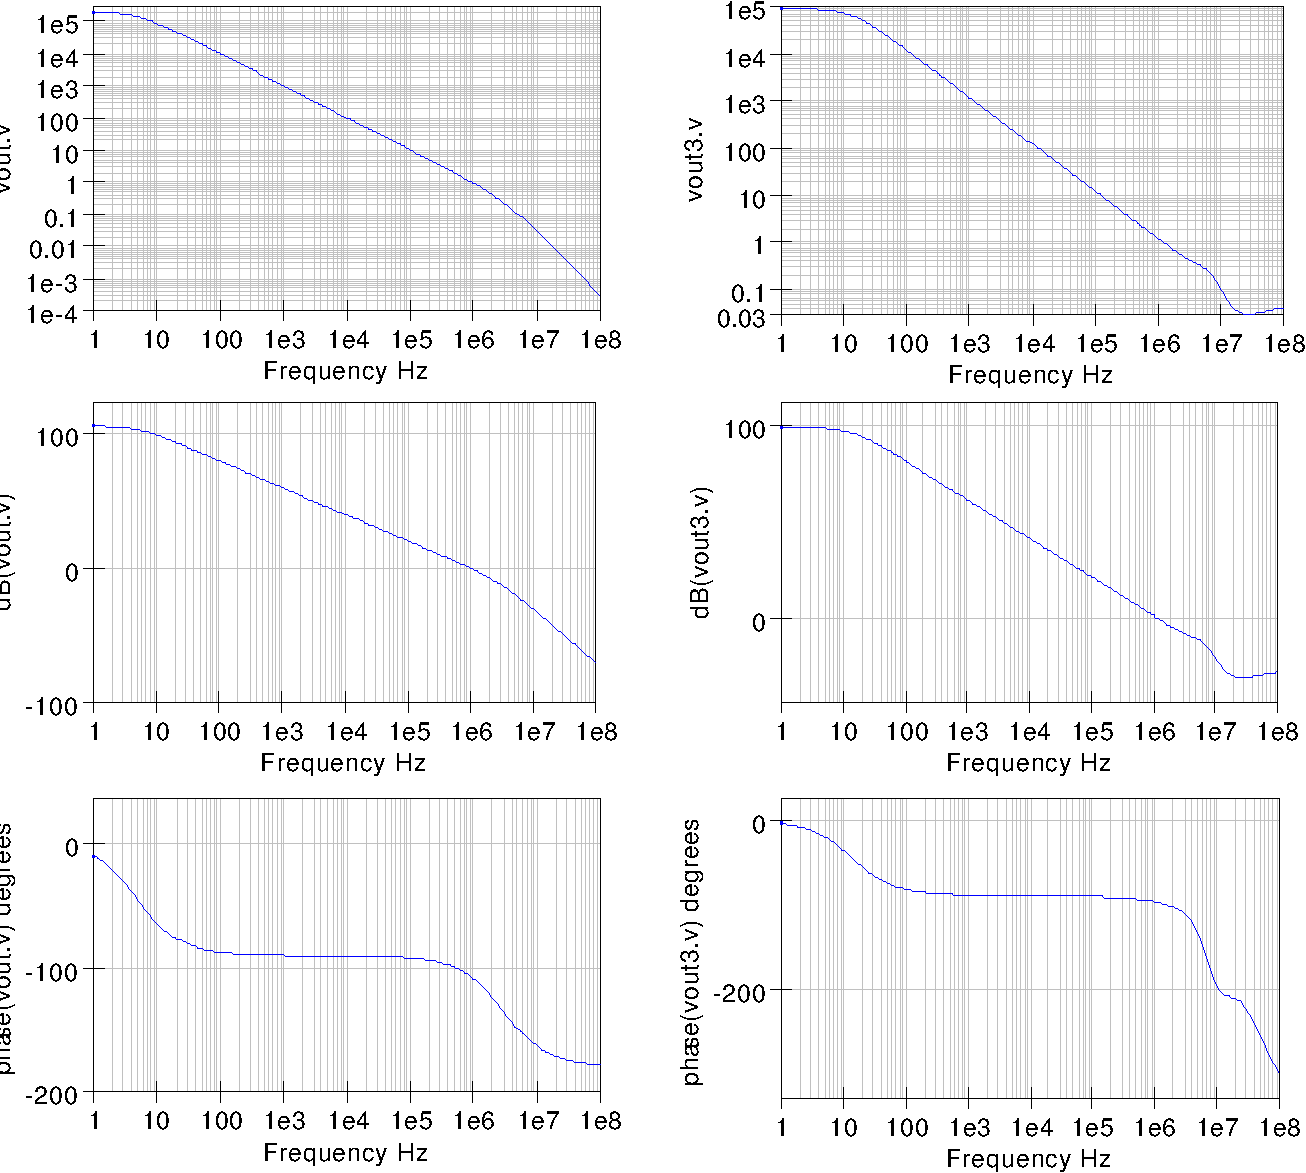
\includegraphics[width=0.9\linewidth]{fig17_dpl}
% tcomb1.png: 99.9998dpi, width=11.35cm, height=3.35cm, bb=0 0 447 132
  \caption{Simulation test results for the circuit shown in Fig.~\ref{fig:opamp16}.}
  \label{fig:opamp17}
\end{figure}

\tutsection{Adding common mode effects to the OP AMP AC macromodel}

The open-loop differential gain $A_{D}(f)$ for most general purpose operational amplifiers can be approximated by

\begin{equation}
A_{D}(f)=AD(0)\dfrac{1}{1+j\dfrac{f}{f_{PD}}}
\end{equation}

Similarly, the common-mode gain $A_{CM}(f)$ can be represented by the same single-pole response and a single zero response given by
\begin{equation}
A_{CM}(f)=A_{CM}(0)\dfrac{1+j\dfrac{f}{f_{CMZ}}}{1+j\dfrac{f}{f_{PD}}}
\end{equation}
Defining the common-mode rejection ratio $CMRR(f)$ of an OP AMP as
\begin{equation}
CMRR(f)=\dfrac{A_{D}(f)}{A_{CM}(f)}
\end{equation}

gives
\begin{equation}
CMRR(f)=CMRR(0)\dfrac{1}{1+j\dfrac{f}{f_{CMZ}}}
\end{equation}
where
\begin{equation}
CMRR(0)=\dfrac{A_{D}(0)}{A_{CM}(0)}
\end{equation}

Common-mode effects can be added to OP AMP macromodels by including a stage in the modular macromodel that introduces a zero in the amplifier frequency response.  Output $V_{CM}$ from the macromodel input stage senses an amplifier common mode signal.  This signal, when passed through a CR network generates the required common mode zero. Figure 18 gives the model of the zero generating network, where.

\begin{enumerate}
\item \textit{RDCMZ} = 650 M$\Omega$ = common-mode input resistance/2.
\item \textit{RCM1 } = 1 M$\Omega$
\item \textit{ECM1}    G = 31.623 = $\dfrac{\dfrac{RCM1}{RCM2}}{CMRR(0)}$. (NOTE: \textit{RCM1/RCM2}is a scaling factor.)
\item \textit{CCM1}  = 795.8 pF = $\dfrac{1}{2\pi*RCM1*f_{CMZ}}$.
\item \textit{RCM2 } = 1 $\Omega$
\end{enumerate}
Typical values for the UA741 OP AMP are:
\begin{enumerate}
\item Common-mode input resistance = 1300 M$\Omega$.
\item \textit{CMRR(0)} =  90 dB 
\item \textit{$f_{CMZ}$} =  200 Hz.
\end{enumerate}


\begin{figure}
  \centering
  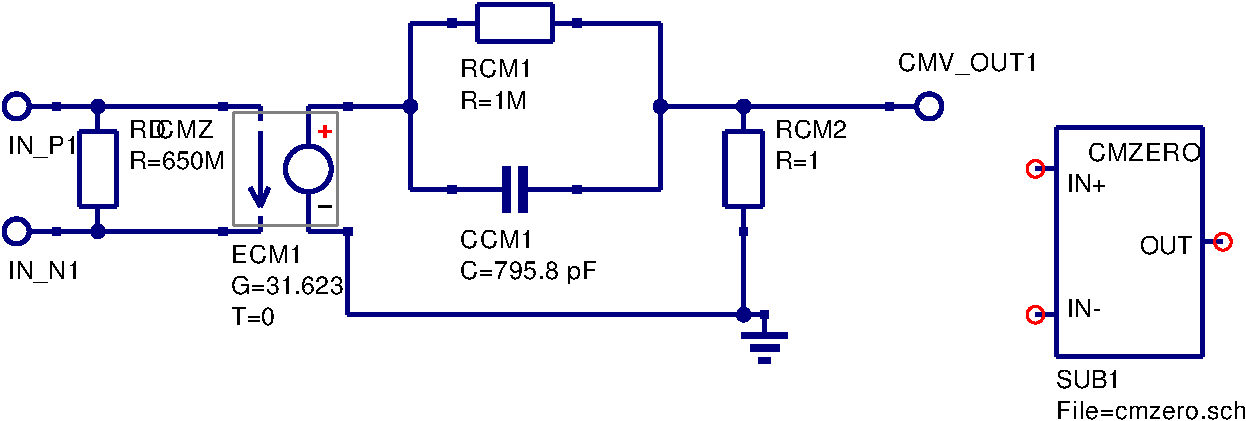
\includegraphics[width=0.9\linewidth]{fig18a_sch}
% tcomb1.png: 99.9998dpi, width=11.35cm, height=3.35cm, bb=0 0 447 132
  \caption{Common-mode zero macromodel}
  \label{fig:opamp18a}
\end{figure}

The AC voltage transfer function for the common-mode zero transfer function is

\begin{equation}
Vout(\verb|CMV_OUT1|)=\dfrac{RCM2}{RCM1}\left[  \dfrac{1+j\omega*RCM1*CCM1}{1+j\omega*RCM2*CCM1}\right] \left[ V(\verb|IN_P1|)-V(\verb|IN_N1|)\right] 
\end{equation}

As $\dfrac{RCM2}{RCM1} << 1$, the pole introduced by the common-mode RC network is at a very high frequency and can be neglected. Combining the common-mode zero with the previously defined stage models yields the macromodel shown in Fig.~\ref{fig:opamp18b}.  In this model the differential and common-mode signals are combined using a simple analogue adder based on voltage conrolled current generators.

\begin{figure}
  \centering
  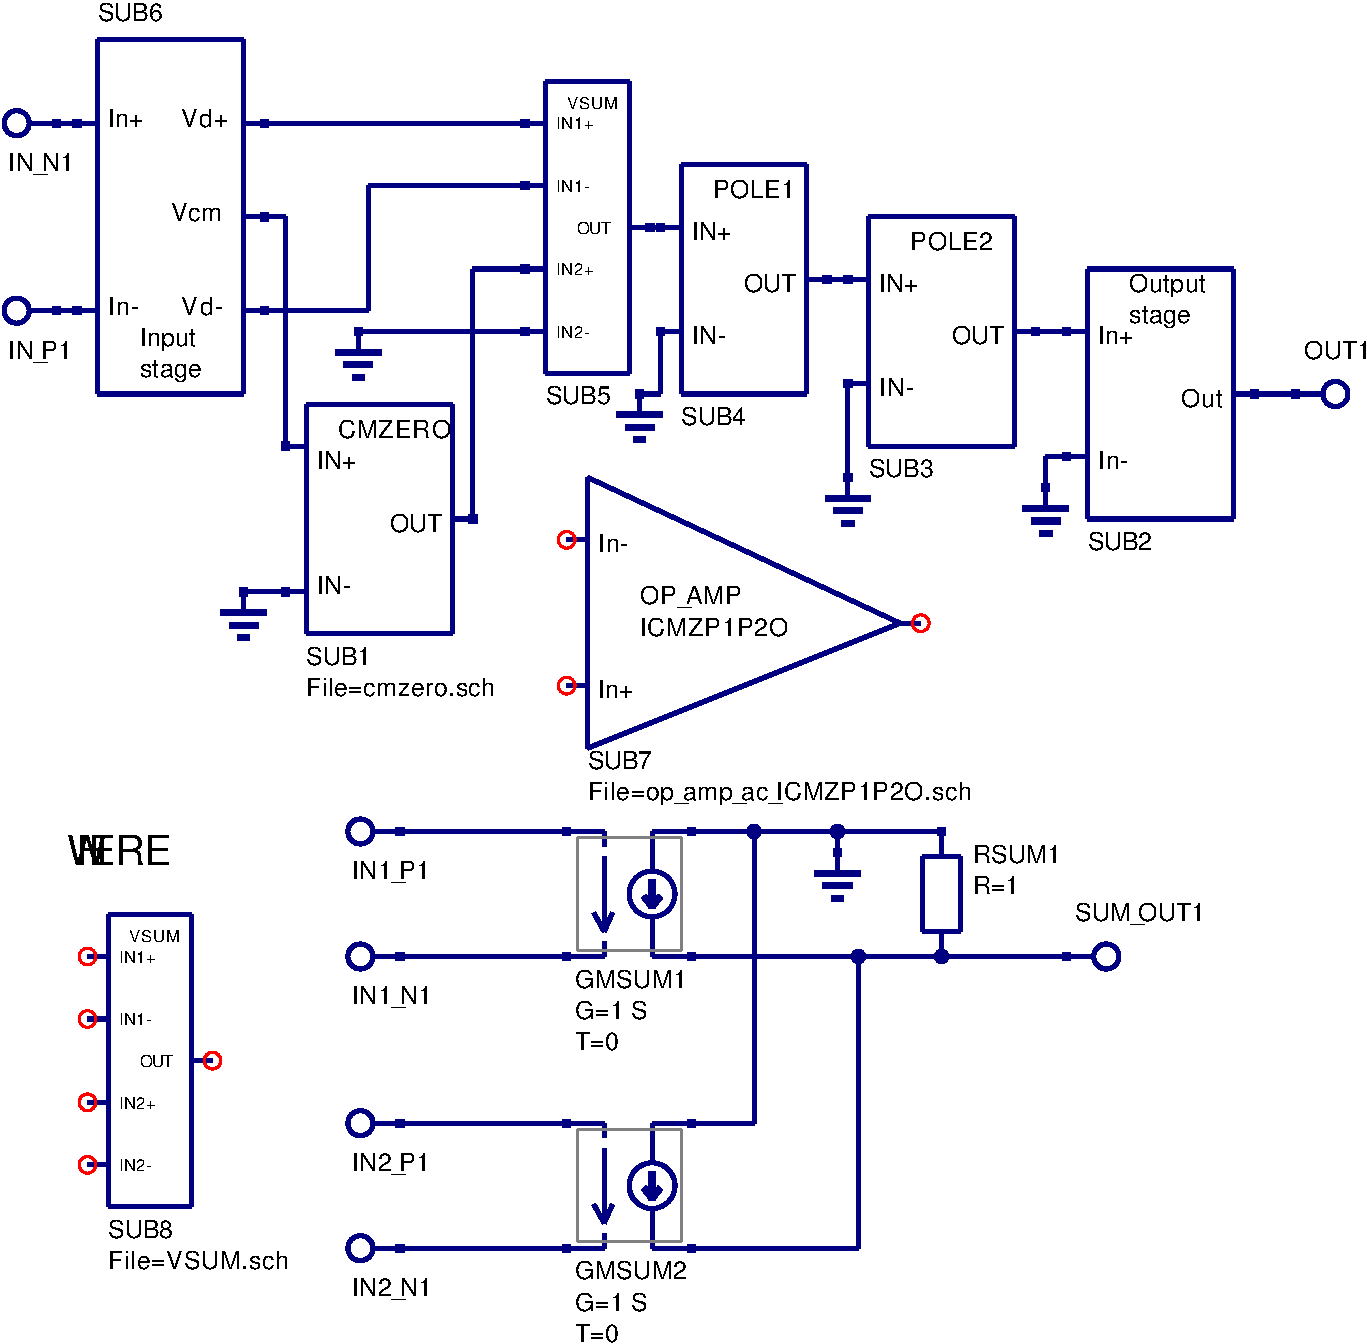
\includegraphics[width=0.9\linewidth]{fig18b_sch}
% tcomb1.png: 99.9998dpi, width=11.35cm, height=3.35cm, bb=0 0 447 132
  \caption{AC macromodel including common-mode zero.}
  \label{fig:opamp18b}
\end{figure}

\tutsubsection{Simulating OP AMP common-mode effects.}
OP AMP common-mode effects can be simulated using the circuit shown in Fig.~\ref{fig:opamp20}.\footnote{Brinson M.E. and Faulkner D.J., New approaches to measurement of operational amplifier common-mode rejection ratio in the frequency domain, IEE Proc-Circuits Devices Sys., Vol 142, NO. 4, August 1995, pp 247-253.} The resulting output voltages (vout.v and vout3.v) for a test circuit with matched resistors are shown plotted in Fig.~\ref{fig:opamp21}, where
$\dfrac{vout(0)}{vin}=\dfrac{1}{CMRR(0)}$.  Clearly the test results for the macromodel and the UA741 transistor model are very similar.  In the case of the macromodel typical device parameters were used to calculate the macromodel component values.  However, in the transistor level model the exact values of the component parameters are unknown.\footnote{The UA741 transistor level model is based on an estimate of the process parameters that determine the UA741 transistor characteristics.  Hence, the device level model is unlikely to be absolutely identical to the model derived from typical parameters values found on OP AMP data sheets. From the simulation results the CMRR(0) values are approximately (1) macromodel 90 dB, (2) UA741 transistor model 101 dB. Similarly, the common-mode zero frequencies are approximately (1) macromodel 200 Hz, (2) UA741 transistor model 500 Hz.}

\begin{figure}
  \centering
  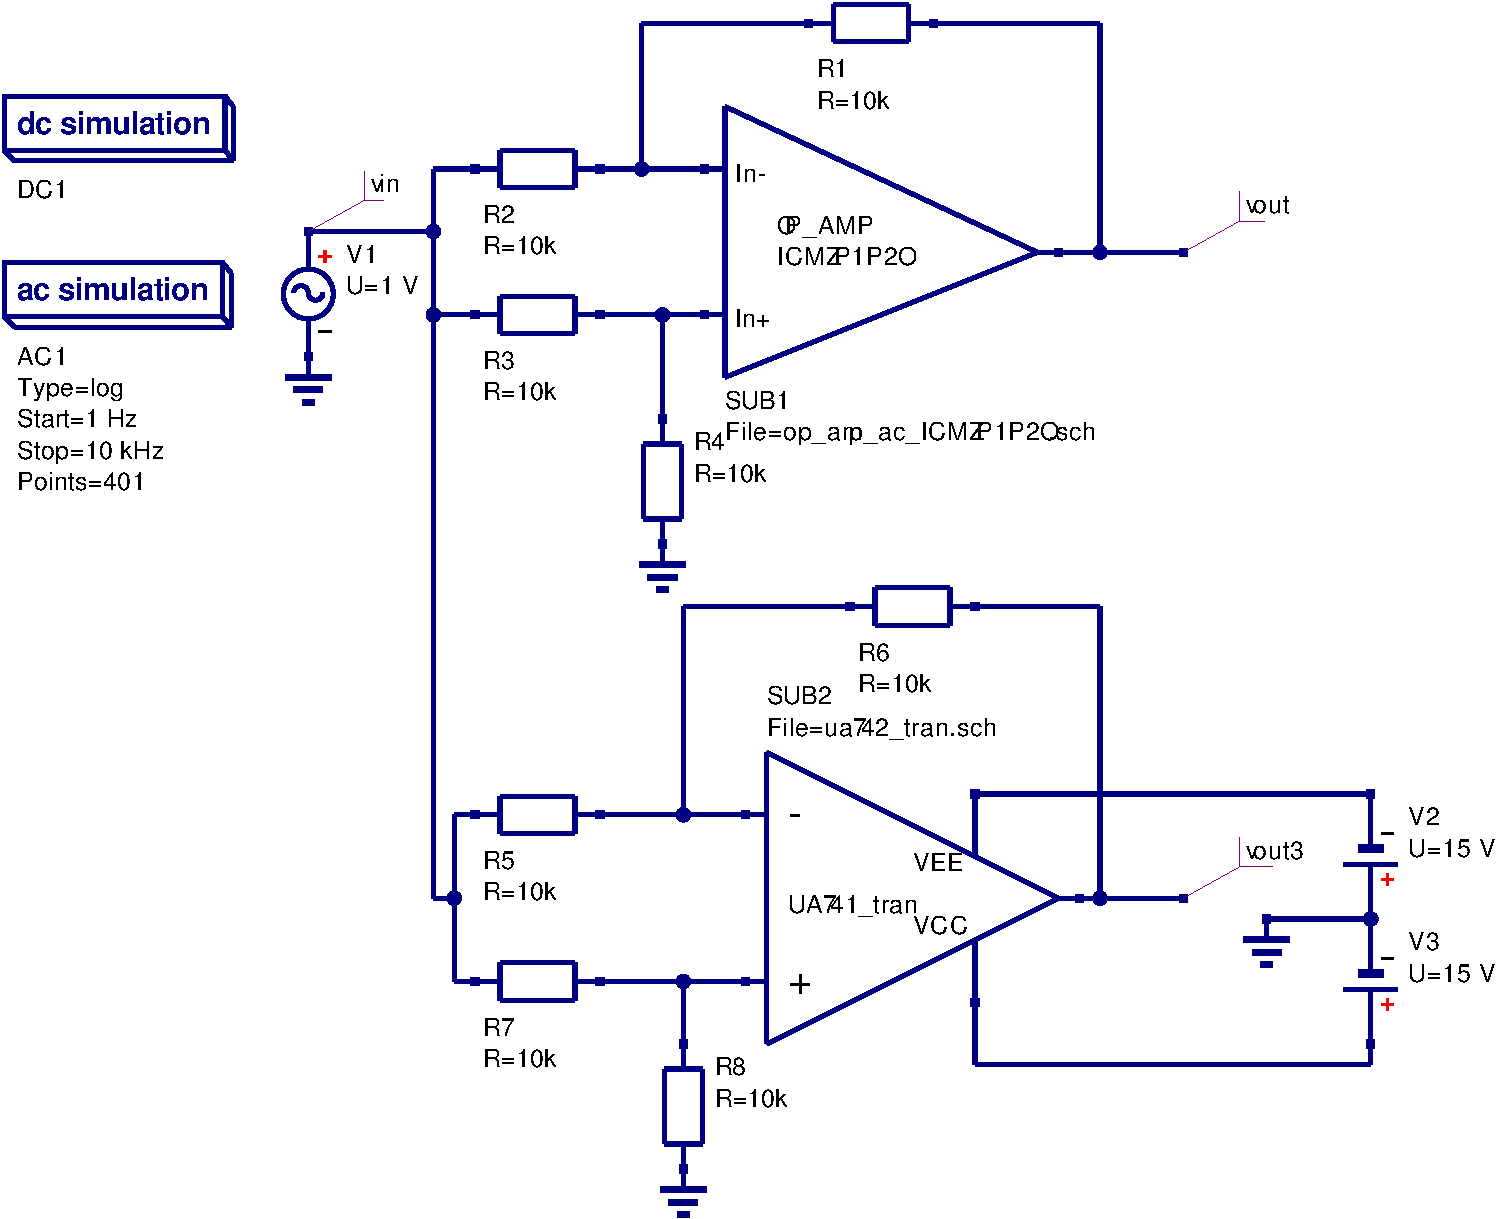
\includegraphics[width=0.9\linewidth]{fig20_sch}
% tcomb1.png: 99.9998dpi, width=11.35cm, height=3.35cm, bb=0 0 447 132
  \caption{Simulation of OP AMP common-mode performance.}
  \label{fig:opamp20}
\end{figure}

\begin{figure}
  \centering
  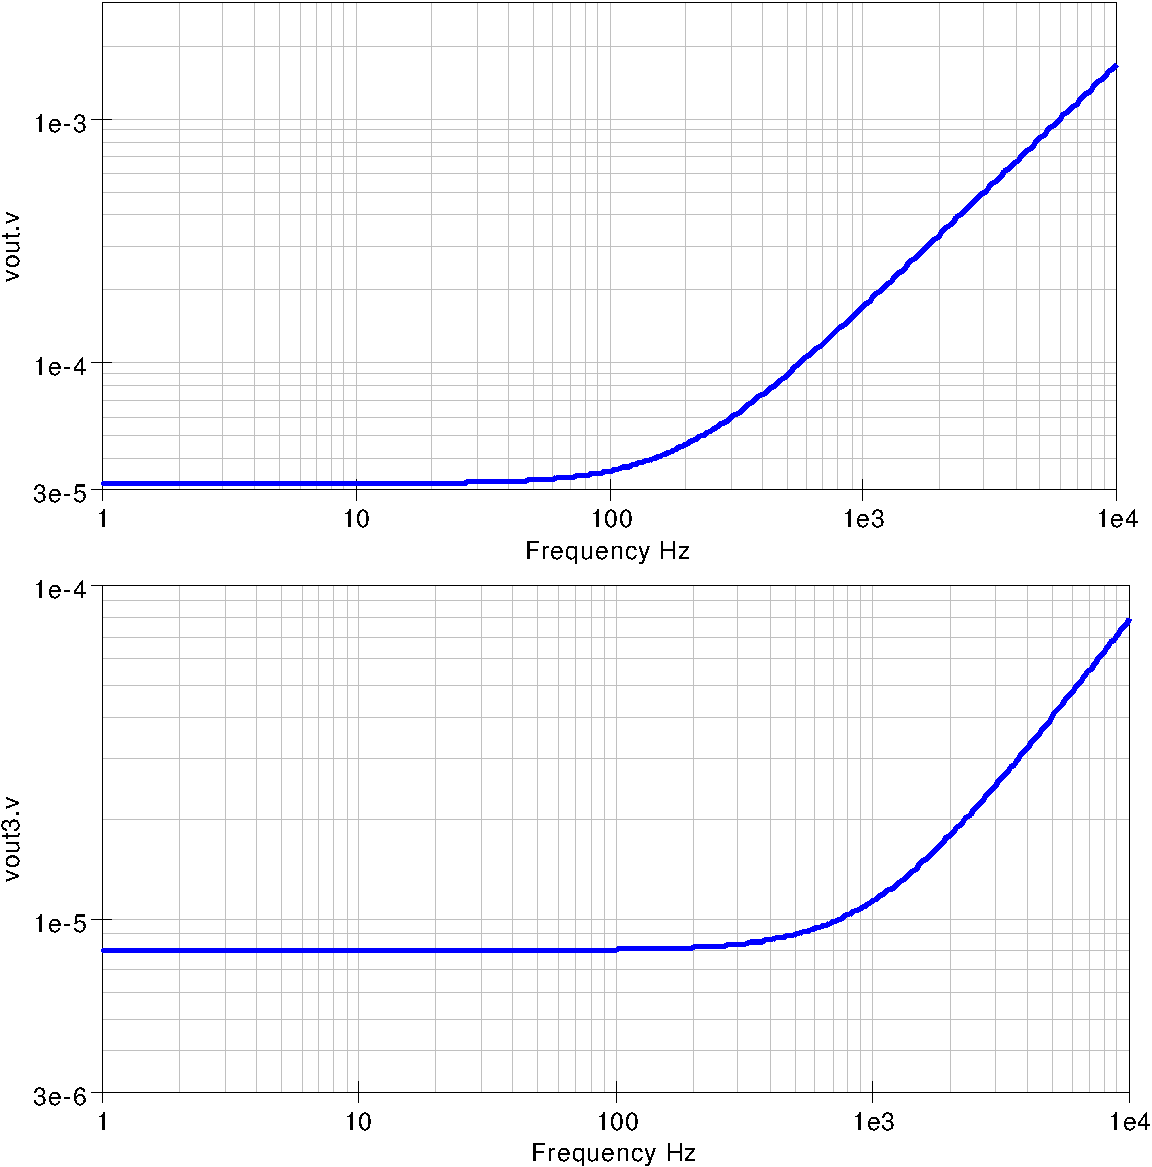
\includegraphics[width=0.9\linewidth]{fig20_dpl}
% tcomb1.png: 99.9998dpi, width=11.35cm, height=3.35cm, bb=0 0 447 132
  \caption{Simulation test results for the circuit shown in Fig.~\ref{fig:opamp20}.}
  \label{fig:opamp21}
\end{figure}



\tutsection{Large signal transient domain OP AMP macromodels}

The modular macromodel introduced in the previous sections concentrated on modelling OP AMP performance in the small signal AC domain. Large signal models need to take into account the passage of signals through an OP AMP in the time domain and limit the excursion of voltage and current swings to the practical values found in actual amplifiers. Starting with the AC domain macromodel introduced in the previous sections, adding a slew rate limiting stage and a overdrive stage will more correctly model OP AMP high speed large signal limitations. Furthermore, by adding output voltage and current limiting stages the OP AMP macromodel will correctly model large signal effects when signal levels approach circuit power supply voltages or the OP AMP output current limits. 

\tutsubsection{Slew rate macromodel derivation.}

The slew rate of an OP AMP can be modelled by limiting the current charging $CP1$ in the first voltage gain stage POLE1. From Fig.~\ref{fig:opamp9}

\begin{equation}
GMP1 \left(  V(IN_{-}P1) - V(IN_{-}N1) \right)  = \dfrac{ V( POLE_{-}1_{-}OUT1 ) } {RADO}+CP1*\dfrac{ dV(POLE_{-}1_{-}OUT1) } {dt} 
\end{equation}

Hence, provided $RADO$ is large\footnote{This condition is normally true because $RADO$ is set to the DC open loop differential gain in macromodule POLE1. }

\begin{equation}
GMP1 \left(  V( IN_{-}P1 ) - V( IN_{-}N1 ) \right)  \simeq  CP1*\dfrac{ dV(POLE_{-}1_{-}OUT1) } {dt}  
\end{equation}


But $ CP1 = \dfrac{1}{2\pi*GBP}$ 


Yielding

\begin{equation}
GMP1 \left(  V(IN_{-}P1) - V(IN_{-}N1) \right)  \simeq \dfrac{1}{2\pi*GBP}*\dfrac{ dV(POLE_{-}1_{-}OUT1) } {dt}  
\end{equation}

Moreover, if $\dfrac{ dV(POLE_{-}1_{-}OUT1)}{dt}$ is set equal to the OP-AMP slew rate then the current\\
 
charging \textit{CP1} will be limited to the maximum allowed. In Fig.~\ref{fig:opamp9} $GMP1$ is 1 S. \\

Therefore, voltage difference  $ V(IN_{-}P1) - V(IN_{-}N1)$\\

must be set to $\dfrac{1}{2\pi*GBP}*\dfrac{ dV(POLE_{-}1_{-}OUT1) } {dt}$.\\

This is done by the network SLEWRT shown in Fig.~\ref{fig:opamp22}, where

\begin{figure}
  \centering
  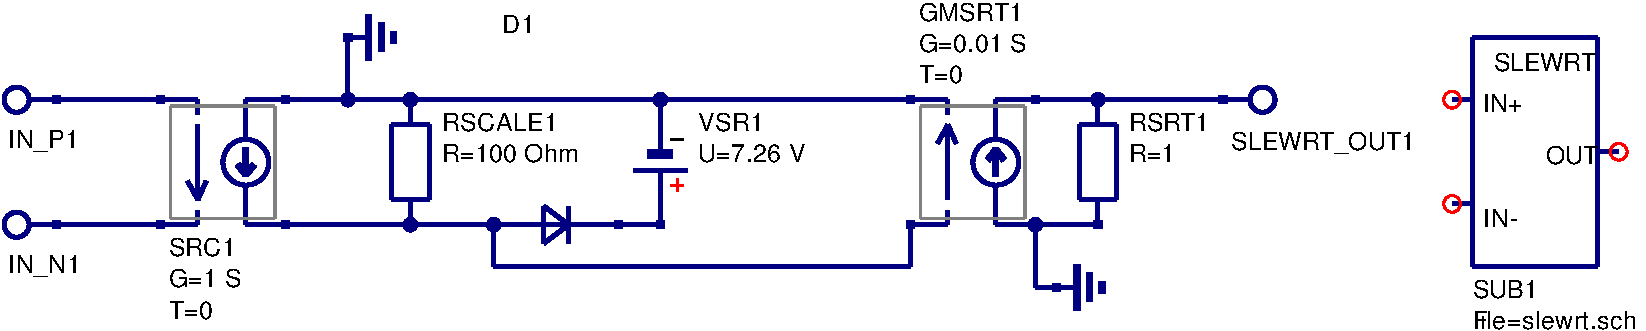
\includegraphics[width=0.9\linewidth]{fig22_sch}
% tcomb1.png: 99.9998dpi, width=11.35cm, height=3.35cm, bb=0 0 447 132
  \caption{OP AMP slew rate macromodel.}
  \label{fig:opamp22}
\end{figure}

\begin{enumerate}
\item \textit{RSCALE1}  = 100 $\Omega$ = Scaling resistance (Scale factor x 100).
\item \textit{SRC1}   G = 1 S.
\item \textit{VSR1}    = V1.
\item \textit{GMSRT1}  G = 0.01 S. (Scale factor = 1/100).
\item \textit{RSRT1}    = 1 $\Omega$
\end{enumerate}
And, 
\begin{enumerate}
\item $V1 = \dfrac{100 * Positive_{-}slew_{-}rate}{2\pi*GBP}-0.7V$
\item $V2 = \dfrac{100 * Negative_{-}slew_{-}rate}{2\pi*GBP}-0.7V$
\item The diode parameters are IS=1e-12 IBV=20mA BV=V1+V2, others default.
\end{enumerate}

Typical values for the UA741 OP AMP are:
\begin{enumerate}
\item $Positive_{-}slew_{-}rate$ = $Negative_{-}slew_{-}rate$ = 0.5V/$\mu$S.
\item $V1$ = $V2$ = 7.25V.
\end{enumerate}

Scaling is used in the slew rate model to allow the use of higher voltages in the clamping circuit. Increased voltages reduce errors due to the forward biased junction voltage. Current limiting results by clamping the voltage across resistor $RSCALE1$ with a diode. This diode acts as a zener diode and saves one nonlinear junction when compared to conventional clamping circuits.  The output section of the SLEWRT circuit removes the internal scaling yielding an overall gain of unity for the module.\\


The circuit in Fig.~\ref{fig:opamp23} demonstrates the effect of slew rate limiting on OP AMP transient performance. Three identical OP AMP inverter circuits are driven from a common input 10 kHz AC signal source. Voltage controlled voltage sources are used to amplify the input signal to the second and third circuits.  The three input signals are (1) 5 V peak, (2) 10 V peak and (3) 15 V peak respectively.  The input and output waveforms for this circuit are illustrated in Fig.~\ref{fig:opamp24}. The effect of slew rate limiting on large signal transient performance is clearly demonstrated by these curves. In the case of the 15 V peak input signal the output signal (vout3.Vt) has a slope that is roughly 0.5 V per $\mu$S. 

\begin{figure}
  \centering
  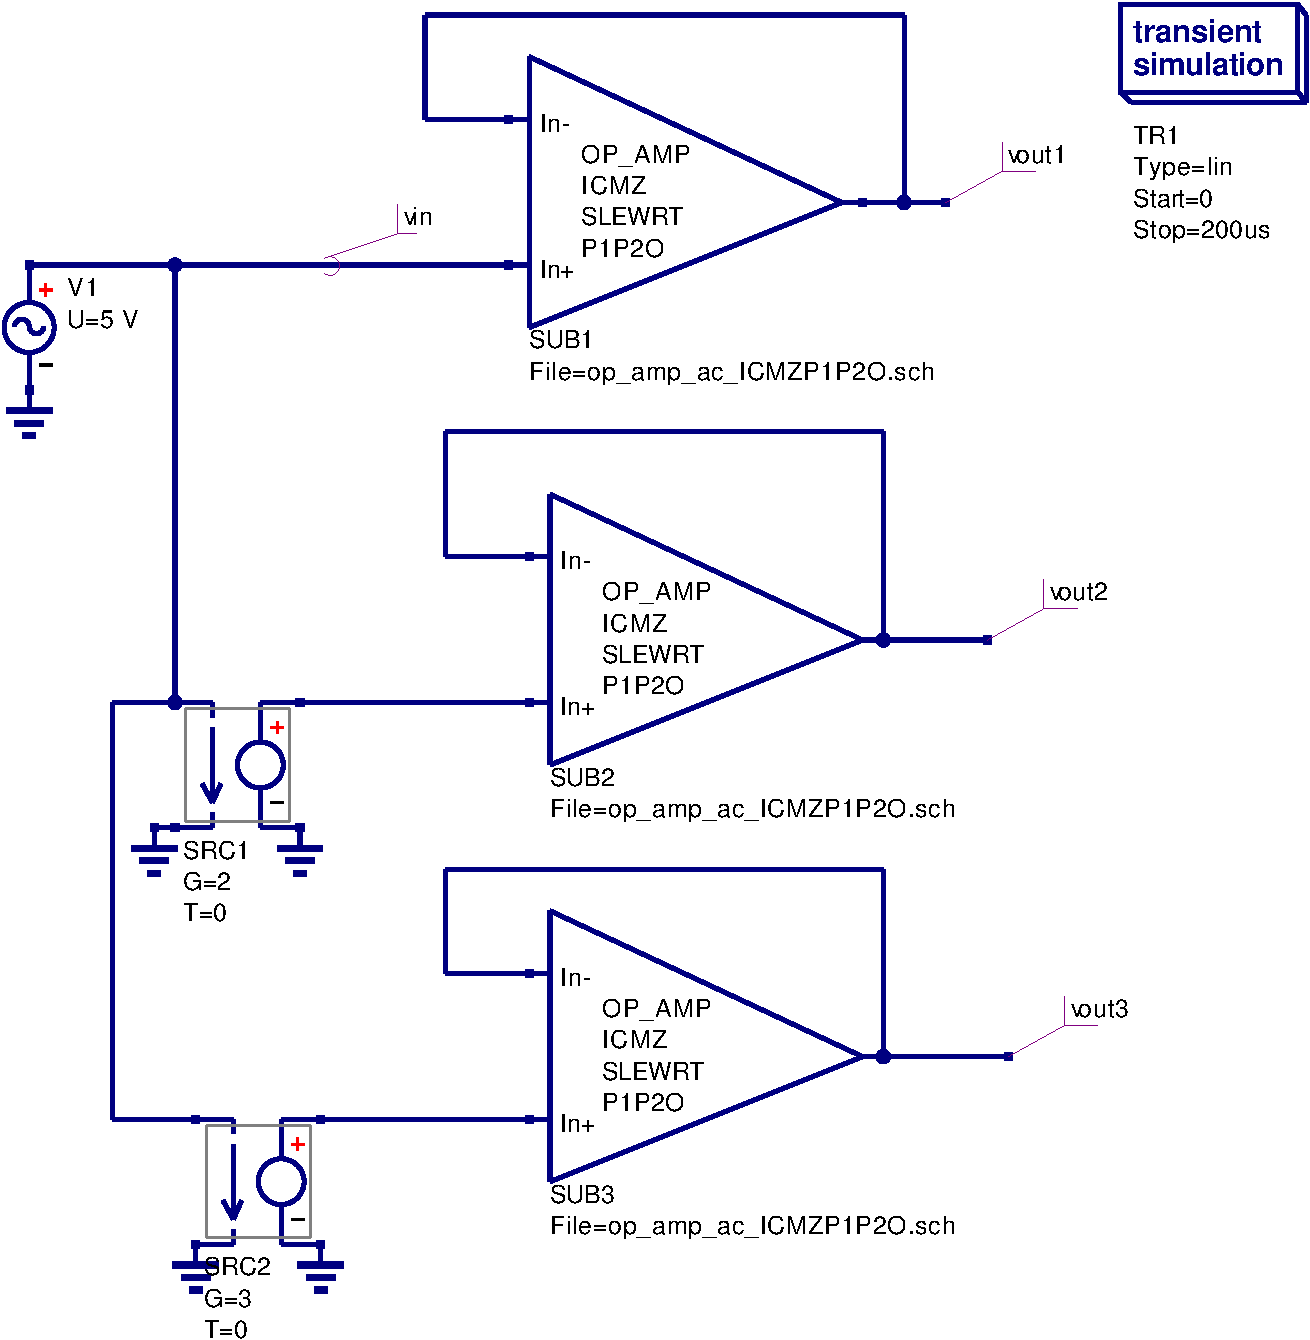
\includegraphics[width=0.9\linewidth]{fig23_sch}
% tcomb1.png: 99.9998dpi, width=11.35cm, height=3.35cm, bb=0 0 447 132
  \caption{OP AMP slew rate test circuit.}
  \label{fig:opamp23}
\end{figure}

\begin{figure}
  \centering
  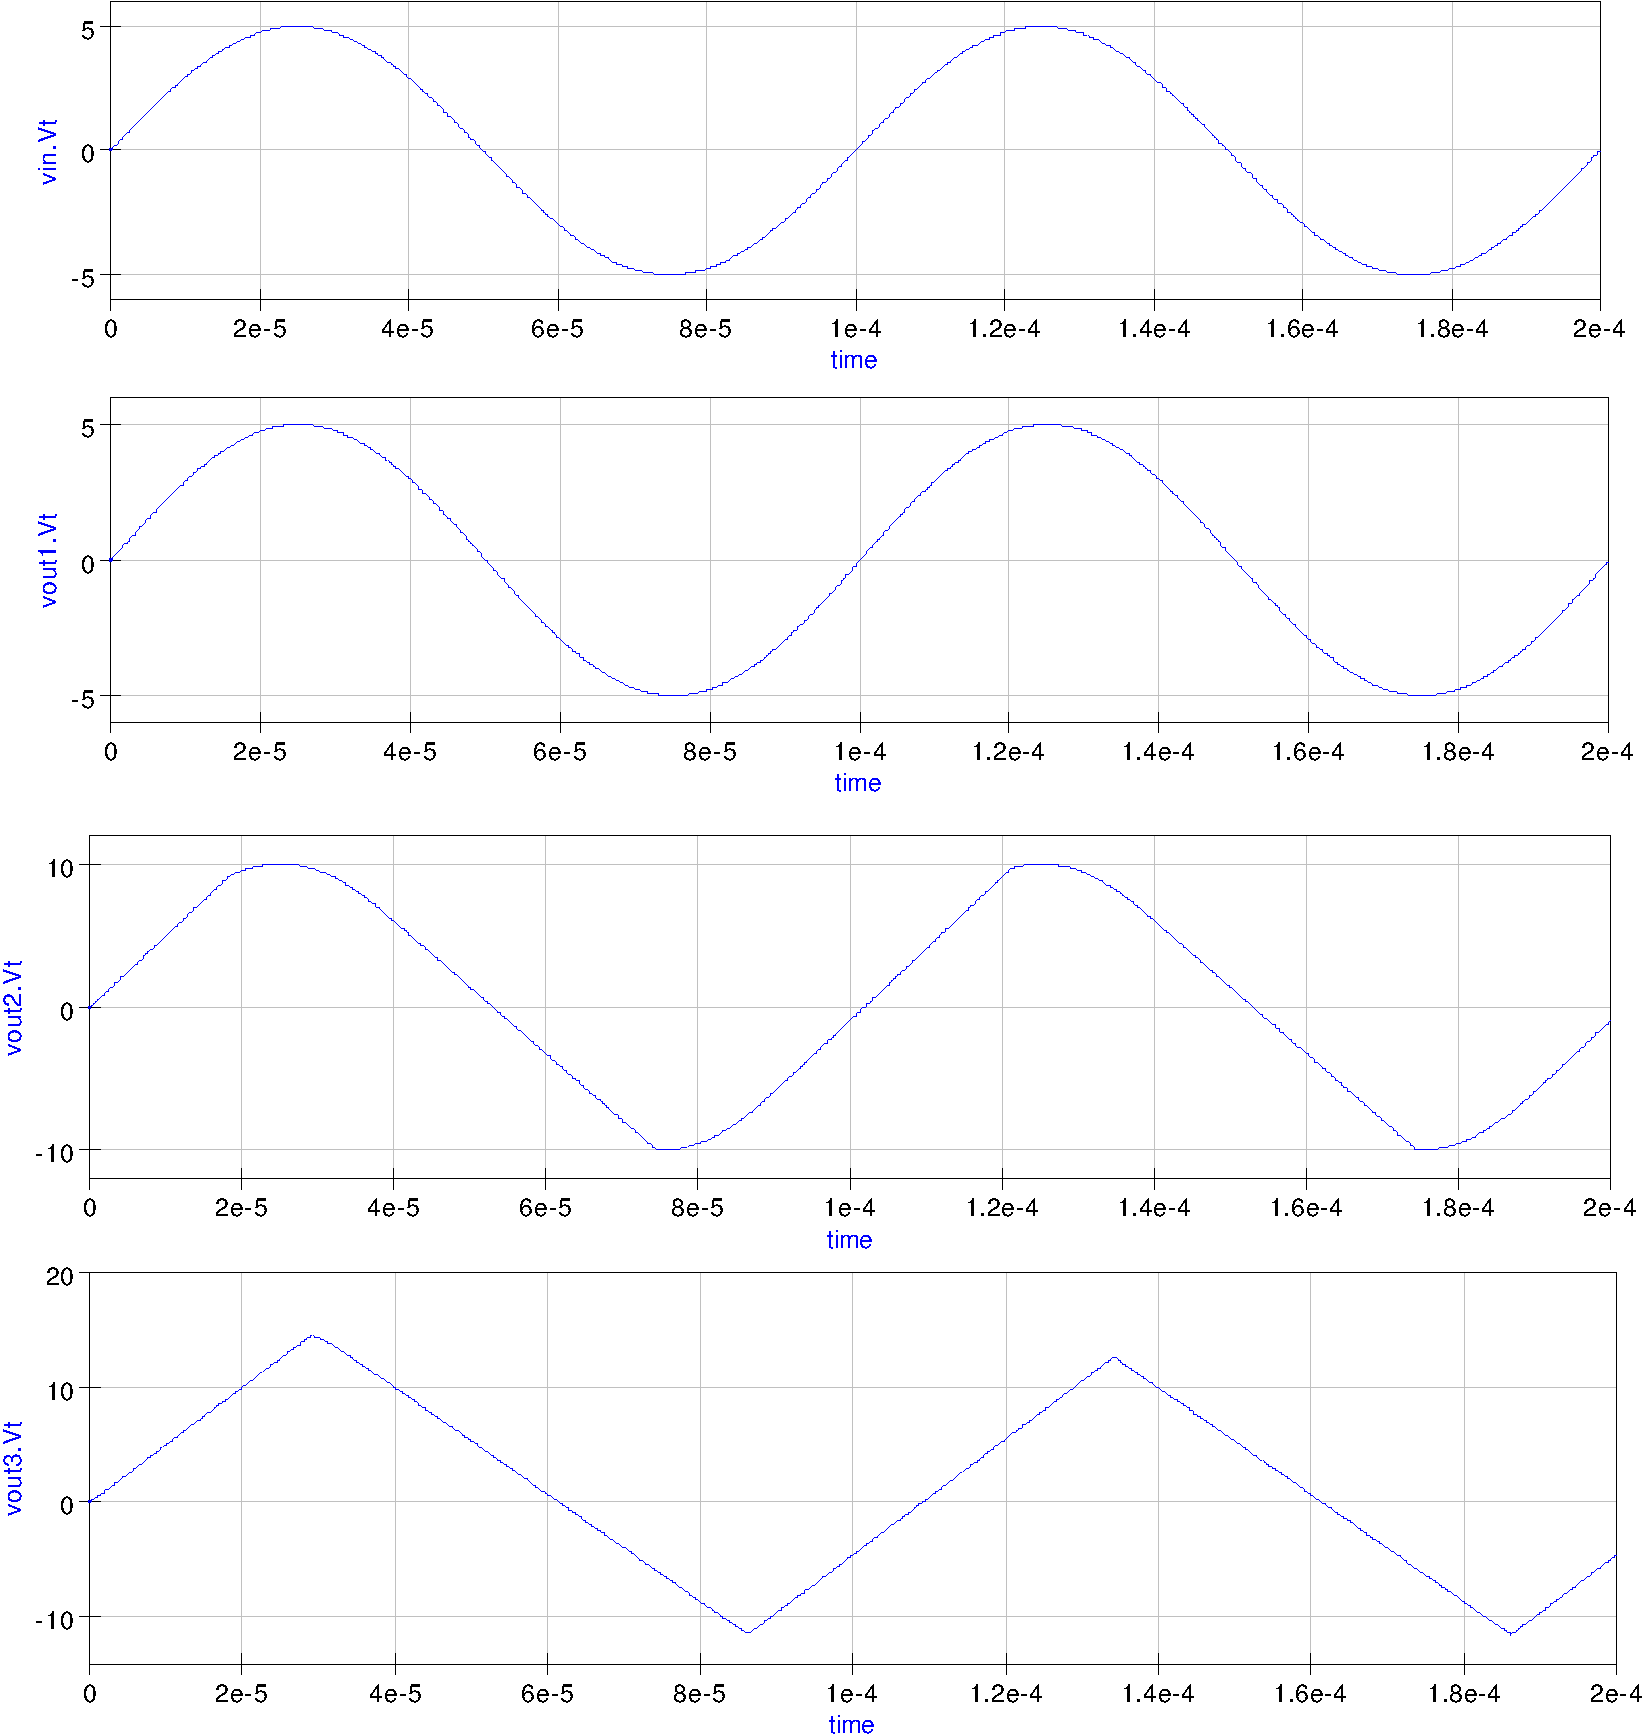
\includegraphics[width=0.9\linewidth]{fig24_dpl}
% tcomb1.png: 99.9998dpi, width=11.35cm, height=3.35cm, bb=0 0 447 132
  \caption{OP AMP slew rate simulation waveforms for the circuit shown in Fig.~\ref{fig:opamp23}.}
  \label{fig:opamp24}
\end{figure}

\tutsubsection{Modelling OP AMP overdrive and output voltage limiting.}

Large transient signals can overdrive an OP AMP causing it's output voltage to saturate. On removal of the overdrive signal an OP AMP takes a finite time to recover\footnote{Overload recovery time of an OP AMP is the time required for the output voltage to recover to a rated output voltage from a saturated condition. Typical values are in the $\mu$ S region.} and return to normal linear circuit behaviour.  When saturated the output voltage is clamped at a voltage close to the plus or minus power rail voltage.  The overdrive and voltage clamping properties of an OP AMP are related and macromodels for both effects need to be added to an OP AMP model when simulating OP AMP overdrive characteristics.  However, in many circuit simulations the overdrive macromodel can be left out without loss of functionality or accuracy.\\

The effect of overdrive signals can be modelled by a voltage clamping circuit which takes account of OP AMP recovery time from voltage overdrive. This extra element clamps the output of the POLE1 module at a level above the OP AMP DC supply voltages. The overall effect of the overdrive circuit is to delay the restoration of linear circuit behaviour when an overload signal is removed.  In contrast to the overdrive module the output voltage limiting module clamps the output voltage to a voltage close to the power rail voltages, clipping any output voltage excursions above the power rail voltage levels. Figure ~\ref{fig:opamp25} illustrates the macromodels for the overdrive and output voltage limiting models, where

\begin{figure}
  \centering
  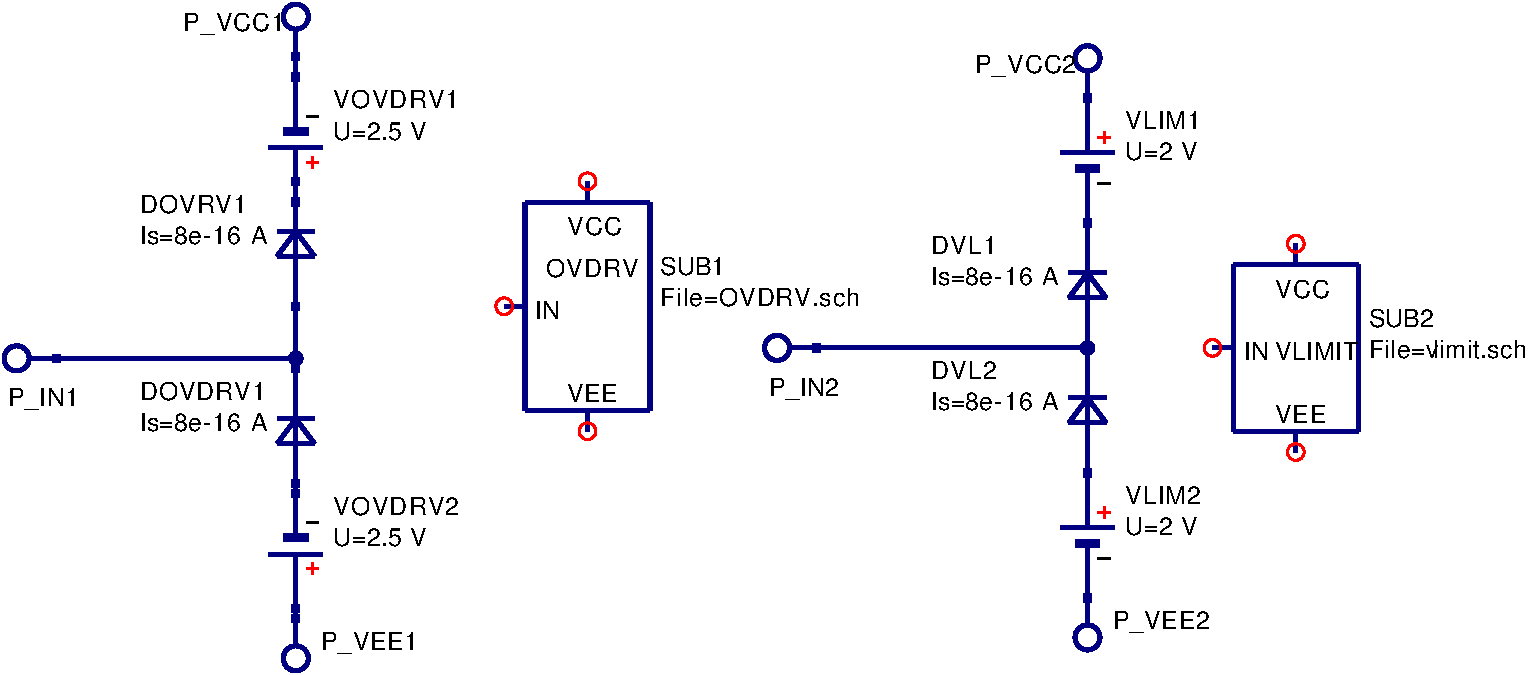
\includegraphics[width=0.9\linewidth]{fig25_sch}
% tcomb1.png: 99.9998dpi, width=11.35cm, height=3.35cm, bb=0 0 447 132
  \caption{OP AMP overdrive and output voltage limiting macromodels.}
  \label{fig:opamp25}
\end{figure}

\begin{enumerate}
\item \textit{VOVDR1} = 2.5 V = (Positive slew rate)*(Amplifier recovery time).
\item \textit{VOVDR2} = 2.5 V = (Negative slew rate)*(Amplifier recovery time).
\item \textit{VLIM1}  = 2.0 V = (+ supply voltage) - (Maximum positive output voltage) + 1 V.
\item \textit{VLIM2}  = 2.0 V = (- supply voltage) - (Maximum negative output voltage) + 1 V.
\item The diode parameters are Is = 8e-16 A, others default.
\end{enumerate}

Typical values for the UA741 OP AMP are:
\begin{enumerate}
\item Amplifier recovery time 5 $\mu$S.
\item + supply voltage =  15 V.
\item - supply voltage = -15 V.
\item Maximum positive output voltage =  14 V.
\item Maximum negative output voltage = -14 V.
\end{enumerate}

The test circuit given in Fig.~\ref{fig:opamp26} illustrates the effects of signal overdrive and output voltage clamping on a unity gain buffer circuit. The test input signal is a 1 kHz signal with the following drive voltages (1) vin1 = 10 V peak, (2) vin2 = 18 V peak, and (3) vin3 = 22 V peak. The corresponding output waveforms are shown in Fig.~\ref{fig:opamp27}. These indicate that increasing overdrive signals results in longer OP AMP recovery times before the amplifier returns to linear behaviour.
\begin{figure}
  \centering
  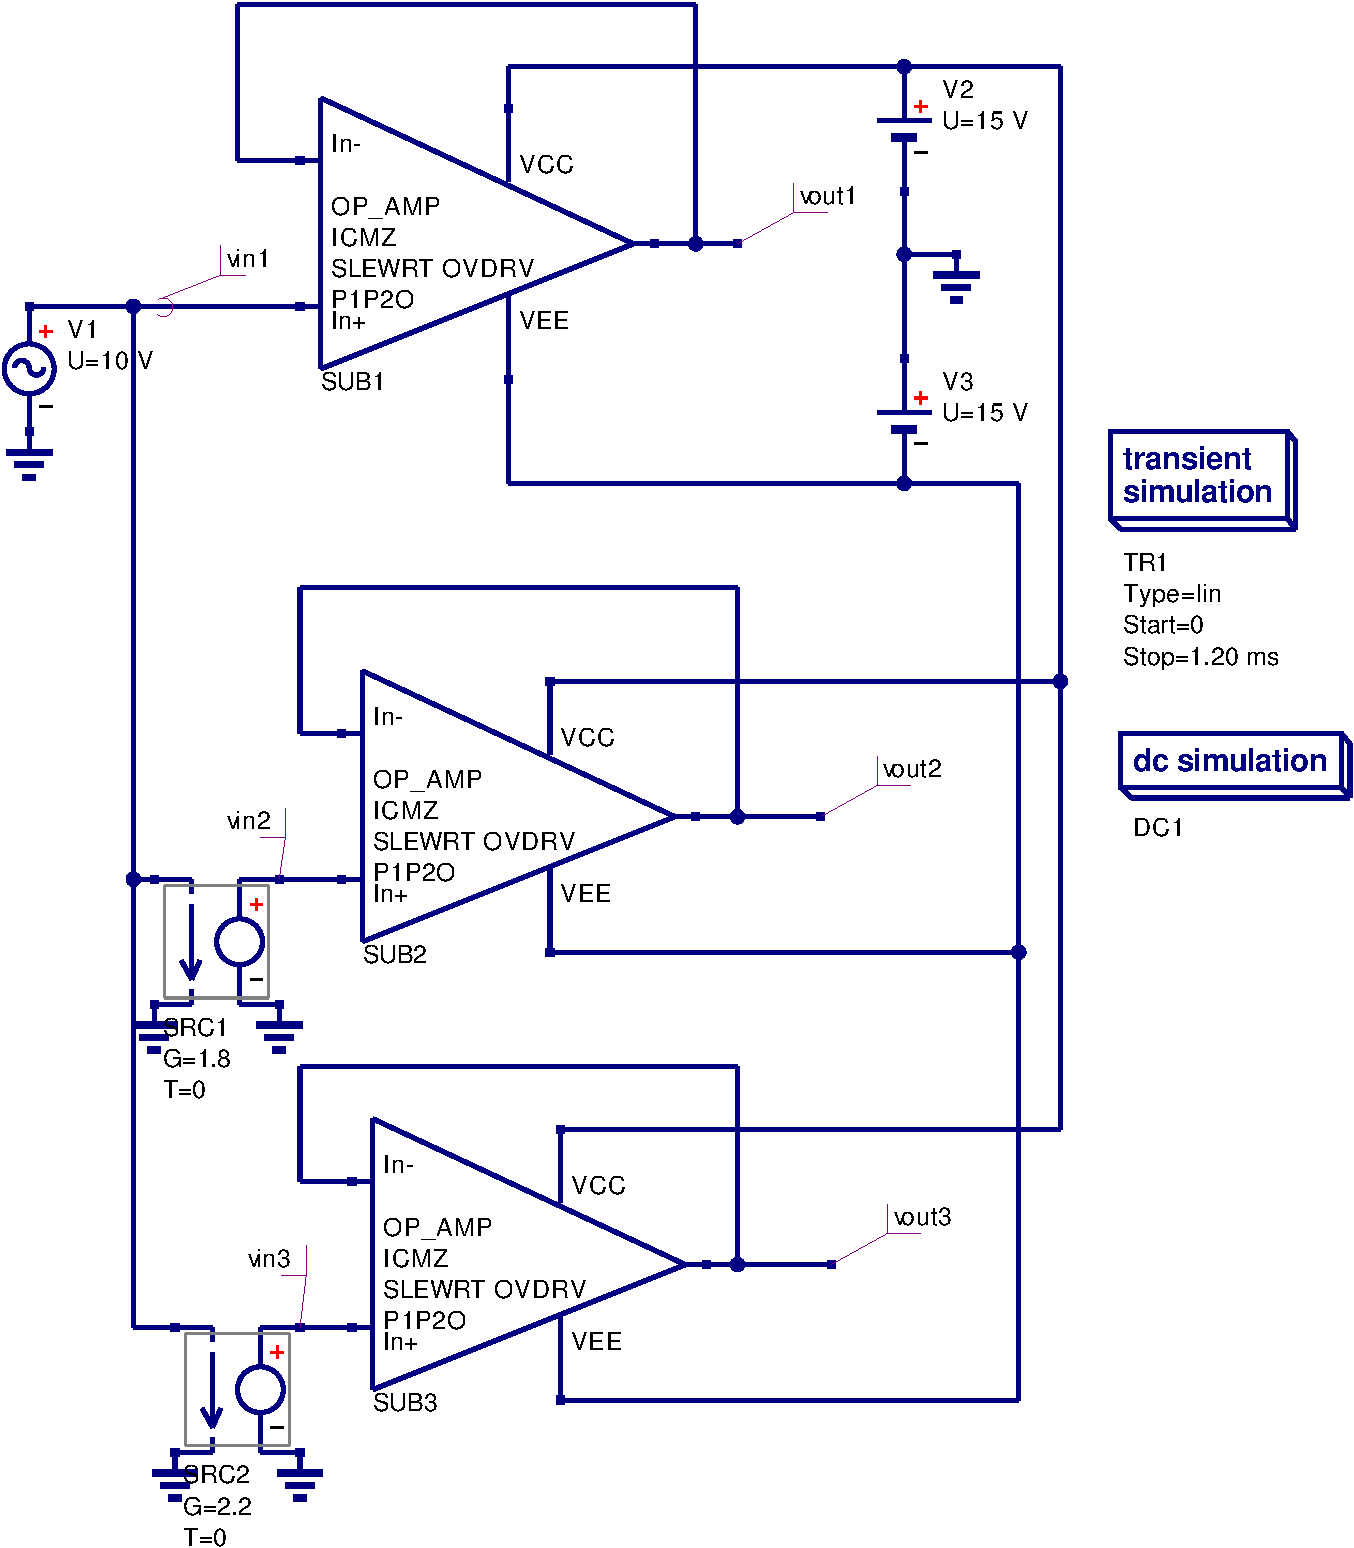
\includegraphics[width=0.9\linewidth]{fig26_sch}
% tcomb1.png: 99.9998dpi, width=11.35cm, height=3.35cm, bb=0 0 447 132
  \caption{OP AMP overdrive and output voltage limiting test circuit.}
  \label{fig:opamp26}
\end{figure}

\begin{figure}
  \centering
  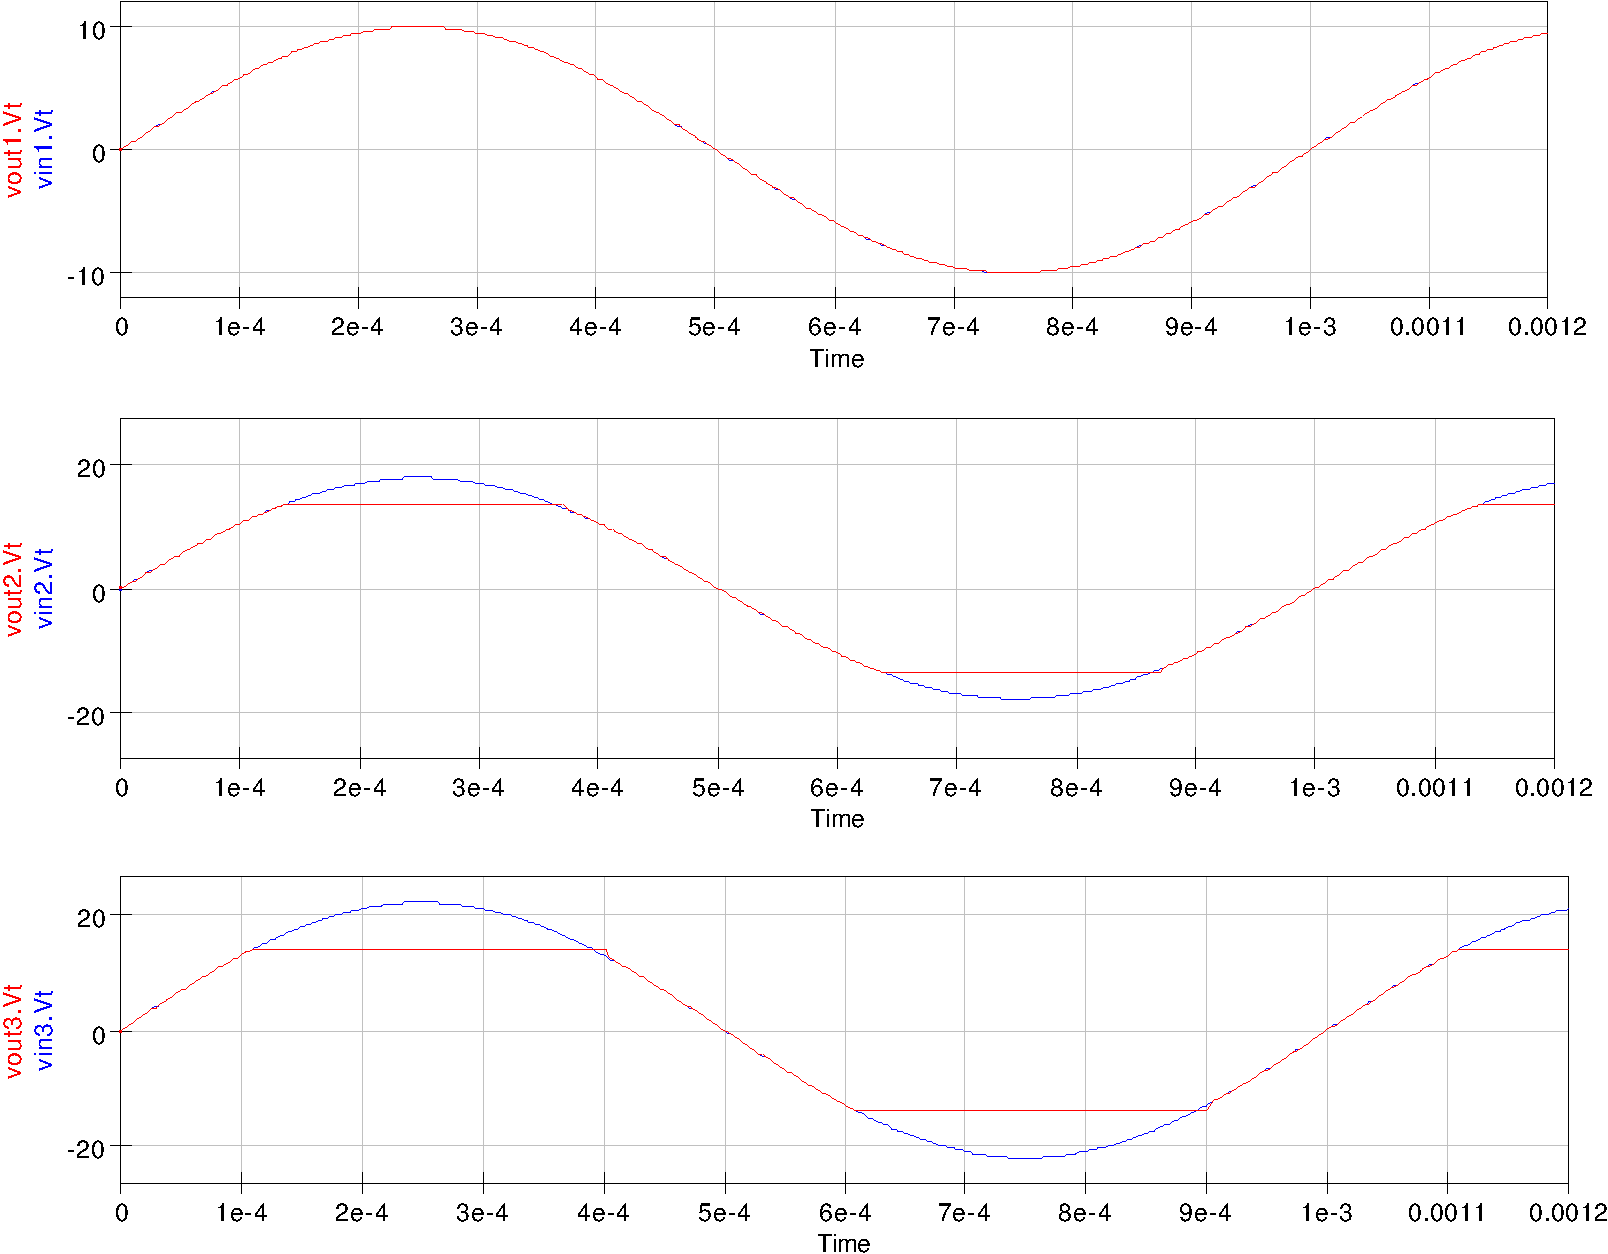
\includegraphics[width=0.9\linewidth]{fig27_dpl}
% tcomb1.png: 99.9998dpi, width=11.35cm, height=3.35cm, bb=0 0 447 132
  \caption{OP AMP overdrive and output voltage limiting waveforms for the circuit shown in Fig.~\ref{fig:opamp26}.}
  \label{fig:opamp27}
\end{figure}

\tutsubsection{Modelling OP AMP output current limiting.}

Most general purpose OP AMPs have a network at the circuit output to protect the device from high load currents generated by shorting the output terminal to ground or some other situation where a high current flows through the OP AMP output stage. The electrical network shown in Fig.~\ref{fig:opamp28} acts as a current limiter: current flowing between pins \verb|P_IN1| and\verb| P_OUT1| is sensed by current controlled voltage generator HCL1. The voltage output from generator HCL1 is in series with voltage controlled generator ECL1. The connection of these generators is in opposite polarity. Hence, when the load current reaches the maximum allowed by the OP AMP either diode DCL1 or DCL2 turns on clamping the OP AMP output voltage preventing the output current from increasing.  The parameters for the current limiter macromodel are given by

\begin{enumerate}
\item \textit{RDCL1} = 100 M$\Omega$ = Dummy resistor.
\item \textit{ECL1}   G = 1.
\item \textit{HCL1}   G = 36$\Omega$ = 0.9 V/(Maximum output current A).
\item The diode parameters are Is = 1e-15 A, others default.
\end{enumerate}
 
A typical value for the UA741 OP AMP short circuit current is 34 mA at $25^{o}$C.\\



\begin{figure}
  \centering
  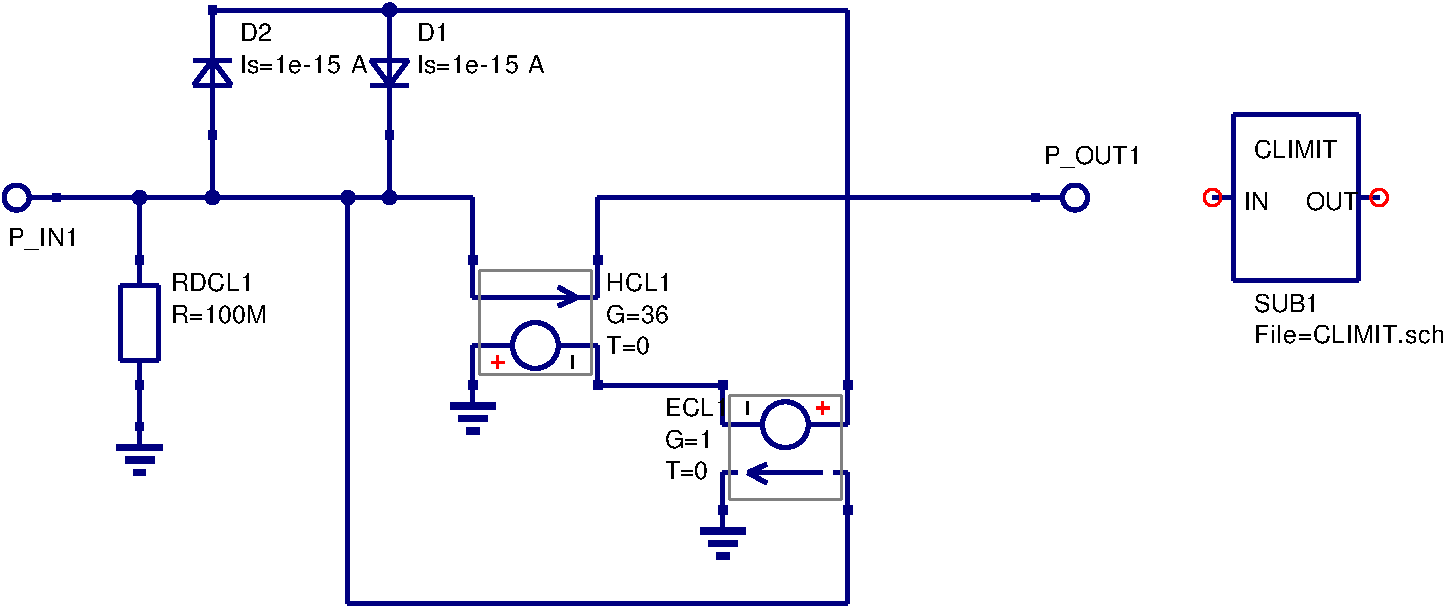
\includegraphics[width=0.9\linewidth]{fig28_sch}
% tcomb1.png: 99.9998dpi, width=11.35cm, height=3.35cm, bb=0 0 447 132
  \caption{OP AMP output current limiter macromodel.} 
  \label{fig:opamp28}
\end{figure}
 Figures~\ref{fig:opamp29} and~\ref{fig:opamp30} show a simple current limiter test circuit and the resulting test waveforms.  
 In this test circuit time controlled switches decrease the load resistors at 1 mS intervals. When the load current reaches
 roughly 34 mA the output voltage is clamped preventing further increases in load current.

\begin{figure}
  \centering
  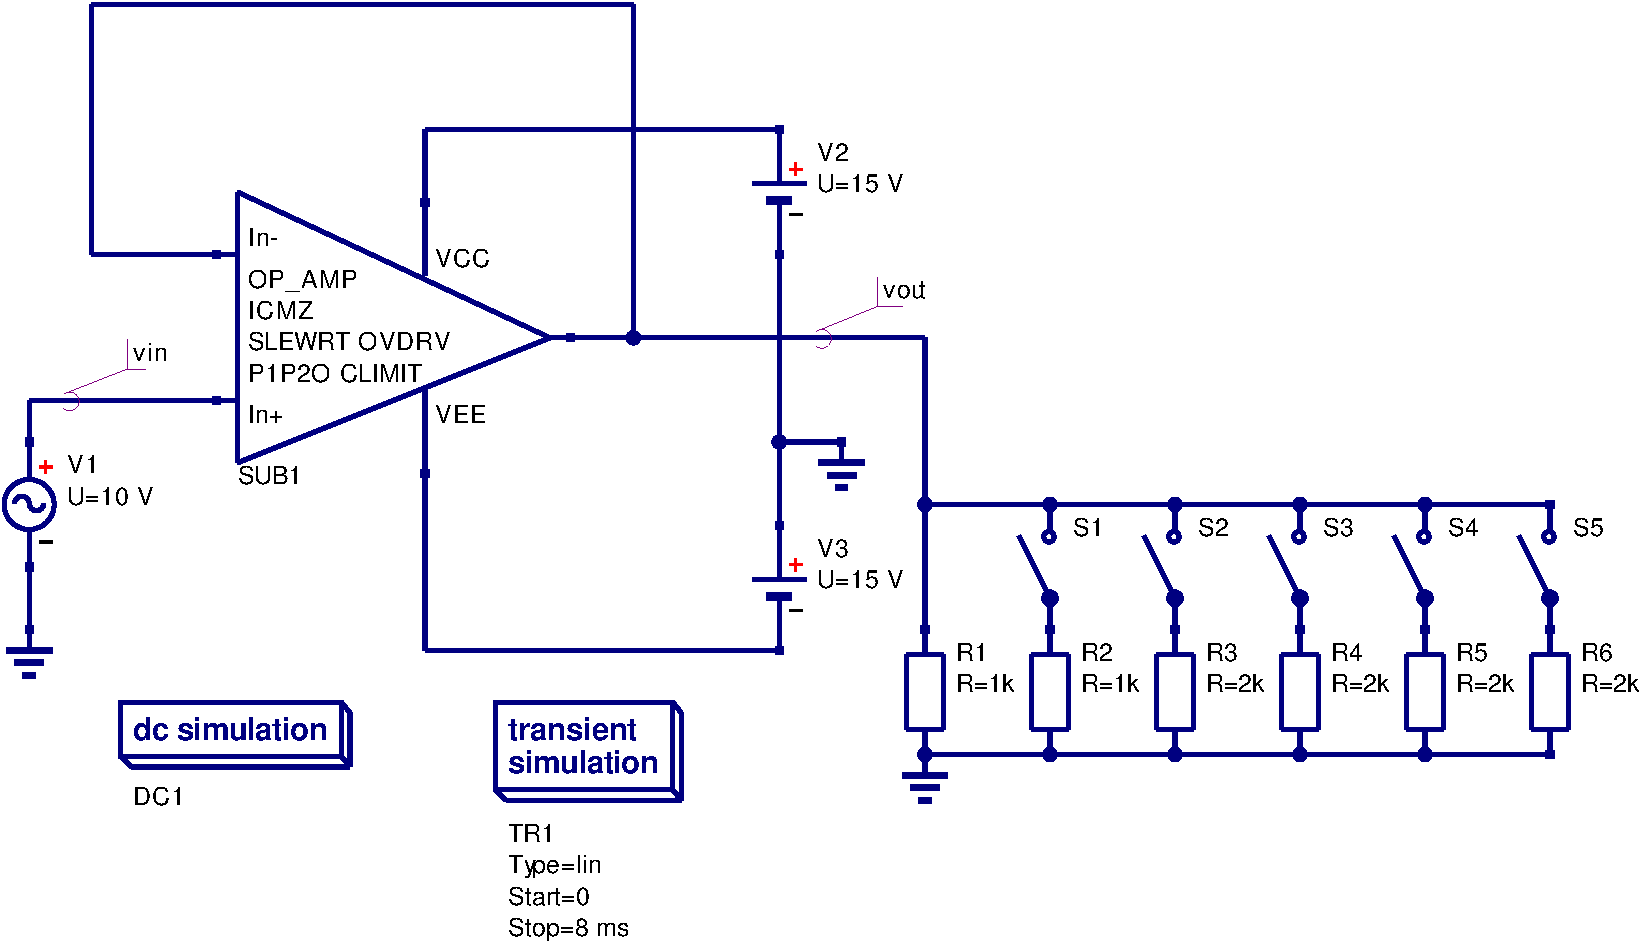
\includegraphics[width=0.9\linewidth]{fig29_sch}
% tcomb1.png: 99.9998dpi, width=11.35cm, height=3.35cm, bb=0 0 447 132
  \caption{OP AMP output current limiter test circuit.} 
  \label{fig:opamp29}
\end{figure}

\begin{figure}
  \centering
  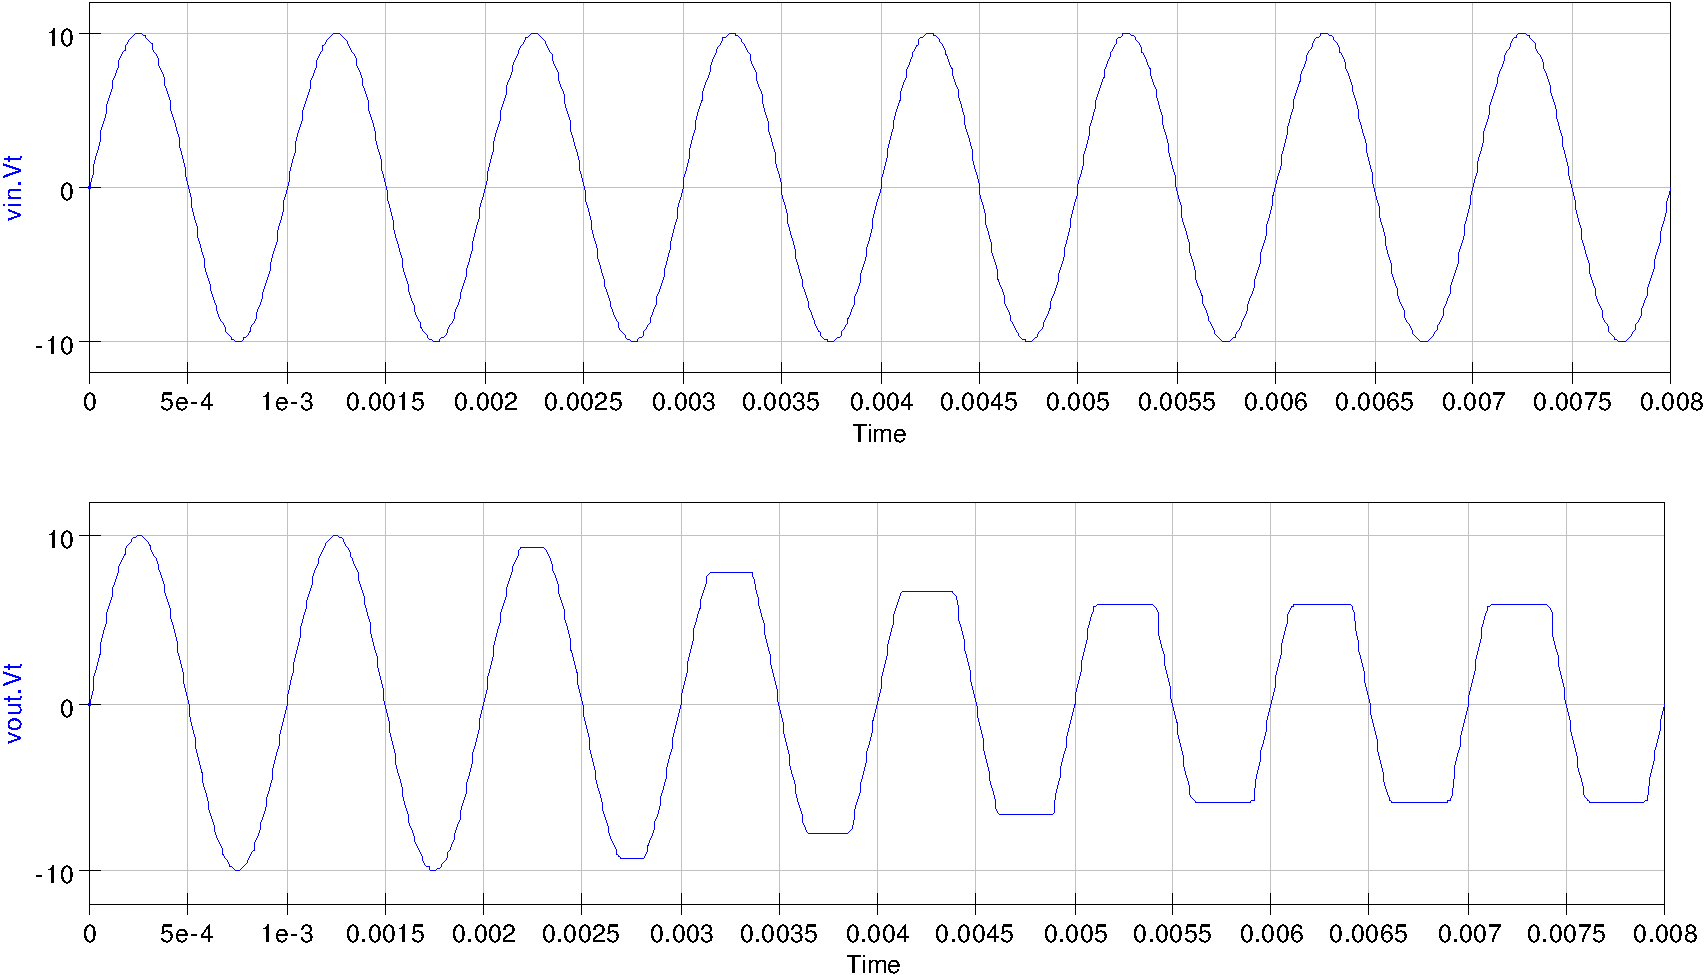
\includegraphics[width=0.9\linewidth]{fig29_dpl}
% tcomb1.png: 99.9998dpi, width=11.35cm, height=3.35cm, bb=0 0 447 132
  \caption{Simulation waveforms for current limiter test circuit shown in Fig.~\ref{fig:opamp29}.} 
  \label{fig:opamp30}
\end{figure}


\begin{table}
\centering
\begin{tabular}{lllllllllll}
Parameter & UA741 & OP27 & OP42 & OPA134 & AD746 & AD826 &  \\ 
Offset voltage (V) & 7e-4 & 30e-6 & 4e-4 & 5e-4 & 3e-4 & 5e-4 &  \\ 
Bias current (A) & 80e-9 & 15e-9 & 130e-12 & 5e-12 & 110e-12 & 3-3e-6 & \\ 
Offset current (A) & 20e-9 & 12e-9 & 6e-12 & 2e-12 & 45e-12 & 25e-9 &  \\ 
Differential input res. (ohm) & 2e6 & 4e6 & 1e12 & 1e13 & 2e11 & 300e3 &  \\ 
Differential input cap. (F) & 1.4e-12 &  & 6e-12 & 2e-12 & 5.5e-12 & 1.5e-12 & \\ 
Avd(0) dB & 106 & 125 & 120 & 120 & 109 & 75 &  \\ 
fp1 (Hz) & 5 & 6 & 20 & 5 & 0.25 & 10e3 &  \\ 
fp2 (Hz) & 3e6 & 17e6 & 20e6 & 10e6 & 35e6 & 100e6 & \\ 
CMRR(0) dB & 90 & 125 & 96 & 100 & 85 & 100 &  \\ 
fcm (Hz) & 200 & 2e3 & 100e3 & 500 & 3e3 & 2e3 &  \\ 
GBP (Hz) & 1e6 & 8e6 & 10e6 & 8e6 & 13e6 & 35e6 & \\ 
Rout (ohm) & 75 & 70 & 50 & 10 & 10 & 8 &  \\ 
Slew rate (V per micro sec.) & 0.5 & 2.8 & 50 & 20 & 75 & 300 &  \\ 
Overdrive recovery time (S) & 5e-6 &   & 700e-9 & 0.5e-6 &   &   & \\ 
DC supply current (A) & 1.4e-3 & 2.5e-3 & 5.1e-3 & 4e-3 & 7e-3 & 6.6e-3 & \\ 
Short circuit output current(A) & 34e-3 & 32e-3 & 30e-3 & 40e-3 & 25e-3 & 90e-3 &  \\ 
Common-mode input res. (ohm) & 1.3e8  & 2e9 &   & 1e13 & 2.5e11 &   &  \\ 
Common-mode input cap. (F) &   &   &   & 5e-12 & 5.5e-12 &   & 
\end{tabular}
\caption{Typical OP AMP parameters taken from device data sheets.}
\label{tab:tab1}
\end{table}

\tutsection{Obtaining OP AMP macromodel parameters from published device data.}
The OP AMP modular macromodel has one very distinct advantage when compared to other amplifier models namely that it is possible to derive the macromodel parameters directly from a common set characteristics found on the majority of manufacturer's data sheets. The data given in Table.~\ref{tab:tab1} shows a typical range of values found on OP AMP data sheets.  In cases where a particular parameter is not given then a starting point is to use a value obtained from a data sheet of an equivalent device. The macromodel element values are then calculated using the equations presented in the previous sections of this tutorial.  As a rule of thumb it is good practice to test each block in the modular macromodel prior to constructing a complete OP AMP macromodel.


\tutsection{More complete design examples.}

In this section two larger design examples are presented. These demonstrate the characteristics of the various OP AMP macromodels introduced in the previous text and attempt to give readers guidance as to the correct model to choose for a particular simulation.

\tutsubsection{Example 1: State variable filter design and simulation} 

The circuit given in Fig.~\ref{fig:opamp31} is a state variable filter which simultaneously generates band-pass, high-pass and low-pass responses. The circuit consists of an OP AMP adder and two integrator circuits and requires three OP AMPS, two capacitors and a number of resistors.  The selection of the type of OP AMP for successful operation of this filter is critical because devices with high offset voltage will cause the integrators to saturate and the circuit will not function correctly. For operation below 20 kHz the OP27 is a good choice of OP AMP because of it's low offset voltage in the $\mu$V region. In this simulation both the DC characteristics and small signal AC transfer characteristics are needed to check the filter design, hence the AC macromodel with the DC parameters embedded in the input stage should allow accurate modelling of the filter performance.\footnote{The magnitude of the output signals from the filter should also be checked to ensure that these signals do not exceed the power supply voltages.}  The insert in Fig.~\ref{fig:opamp31} list the DC output voltages for each of the OP AMP stages indicating that the integrators are not saturated.  The design of the state variable filter uses the following equations:
\begin{enumerate}
\item The superposition principle yields
\begin{equation}
vhp = -\dfrac{R1}{R6}vin-\dfrac{R1}{R7}vlp+\left( 1+\dfrac{R1}{R7 \parallel R6} \right) \dfrac{R4}{R4+R5}vbp
\end{equation}
When $R1= R6 =R7$

\begin{equation}
vhp = -vin -vlp +  \dfrac{3R4}{R4+R5}vbp
\end{equation}

\item Also
\begin{equation}
vbp = -\dfrac{1}{j\frac{f}{f_{0}}}vhp
\end{equation}
where 
\begin{equation}
f_{0}=\dfrac{1}{2 \pi R_{2}C_{1}} = \dfrac{1}{2 \pi R_{3}C_{2}}
\end{equation} 

\item Similarly
\begin{equation}
vlp = -\dfrac{1}{j\frac{f}{f_{0}}}vbp = -\dfrac{1}{(\frac{f}{f_{0}})^{2}}vhp  
\end{equation}

\item Hence
\begin{equation}
\dfrac{vhp}{vin}=\dfrac{(\frac{f}{f_{0}})^{2}}{1-(\frac{f}{f_{0}})^{2}+(\frac{j}{Q})(\frac{f}{f_{0}})}
\end{equation}
Where
\begin{equation}
Q = \dfrac{1}{3}(1+\dfrac{R5}{R4})
\end{equation}

\item Also
\begin{equation}
\dfrac{vbp}{vin}=\dfrac{j\frac{f}{f_{0}}}{1-(\frac{f}{f_{0}})^{2}+(\frac{j}{Q})(\frac{f}{f_{0}})}
\end{equation}

\item Also
\begin{equation}
\dfrac{vlp}{vin}=\dfrac{-1}{1-(\frac{f}{f_{0}})^{2}+(\frac{j}{Q})(\frac{f}{f_{0}})}
\end{equation}

\end{enumerate}

Assuming $f_{0}$ = 1 kHz and the required bandwidth of the band pass filter is 10 Hz, on setting $R1 = R6 = R7 = 47 k\Omega$ and $C1 = C2 = 2.2 nF$, calculation yields $R2 = R3 = 72.33 k\Omega$\footnote{The values of $R2$ and $R3$ need to be trimmed if the filter center frequency and bandwidth are required to high accuracy.}  In this design $Q = 1k/10 = 100$.  Hence setting $R4 = 1k\Omega$ yields $R5 = 294k\Omega$ (1 \verb|%| tolerance). The simulation waveforms for the band pass output are given in Fig.~\ref{fig:opamp32} \footnote{Note that the input signal $vin$ has been set at 0.1 V peak.  The circuit has a Q factor of 100 which means that the band pass output voltage is 10 V peak. Input signals of amplitude much greater than 0.1 V are likely to drive the output signal into saturation when the power supply voltages are $\pm15 V$.}.  When the circuit Q factor is reduced to lower values the other filter outputs act as traditional high and low pass filters. The simulation results for Q factor one are shown in Fig.~\ref{fig:opamp33}.
\begin{figure}
  \centering
  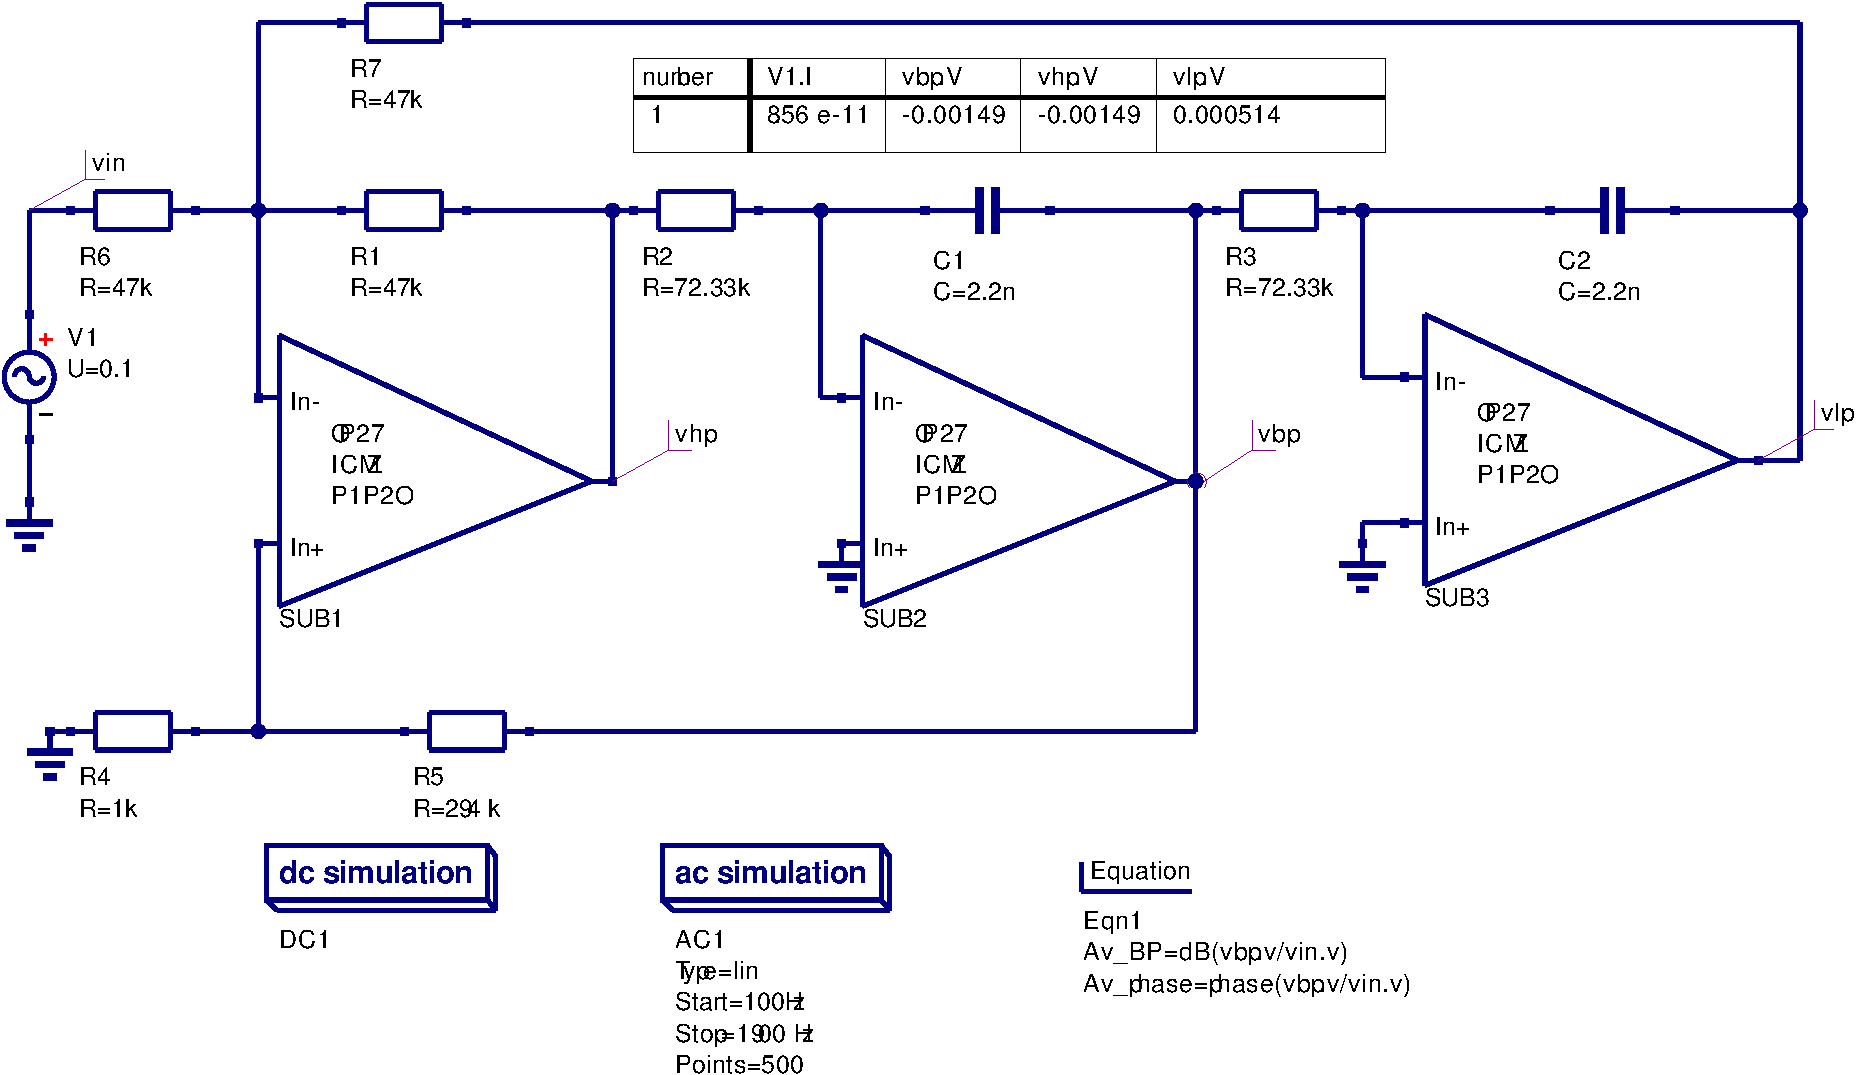
\includegraphics[width=0.9\linewidth]{fig31_sch} 
% tcomb1.png: 99.9998dpi, width=11.35cm, height=3.35cm, bb=0 0 447 132
  \caption{Three OP AMP state variable filter.} 
  \label{fig:opamp31}
\end{figure}

\begin{figure}
  \centering
  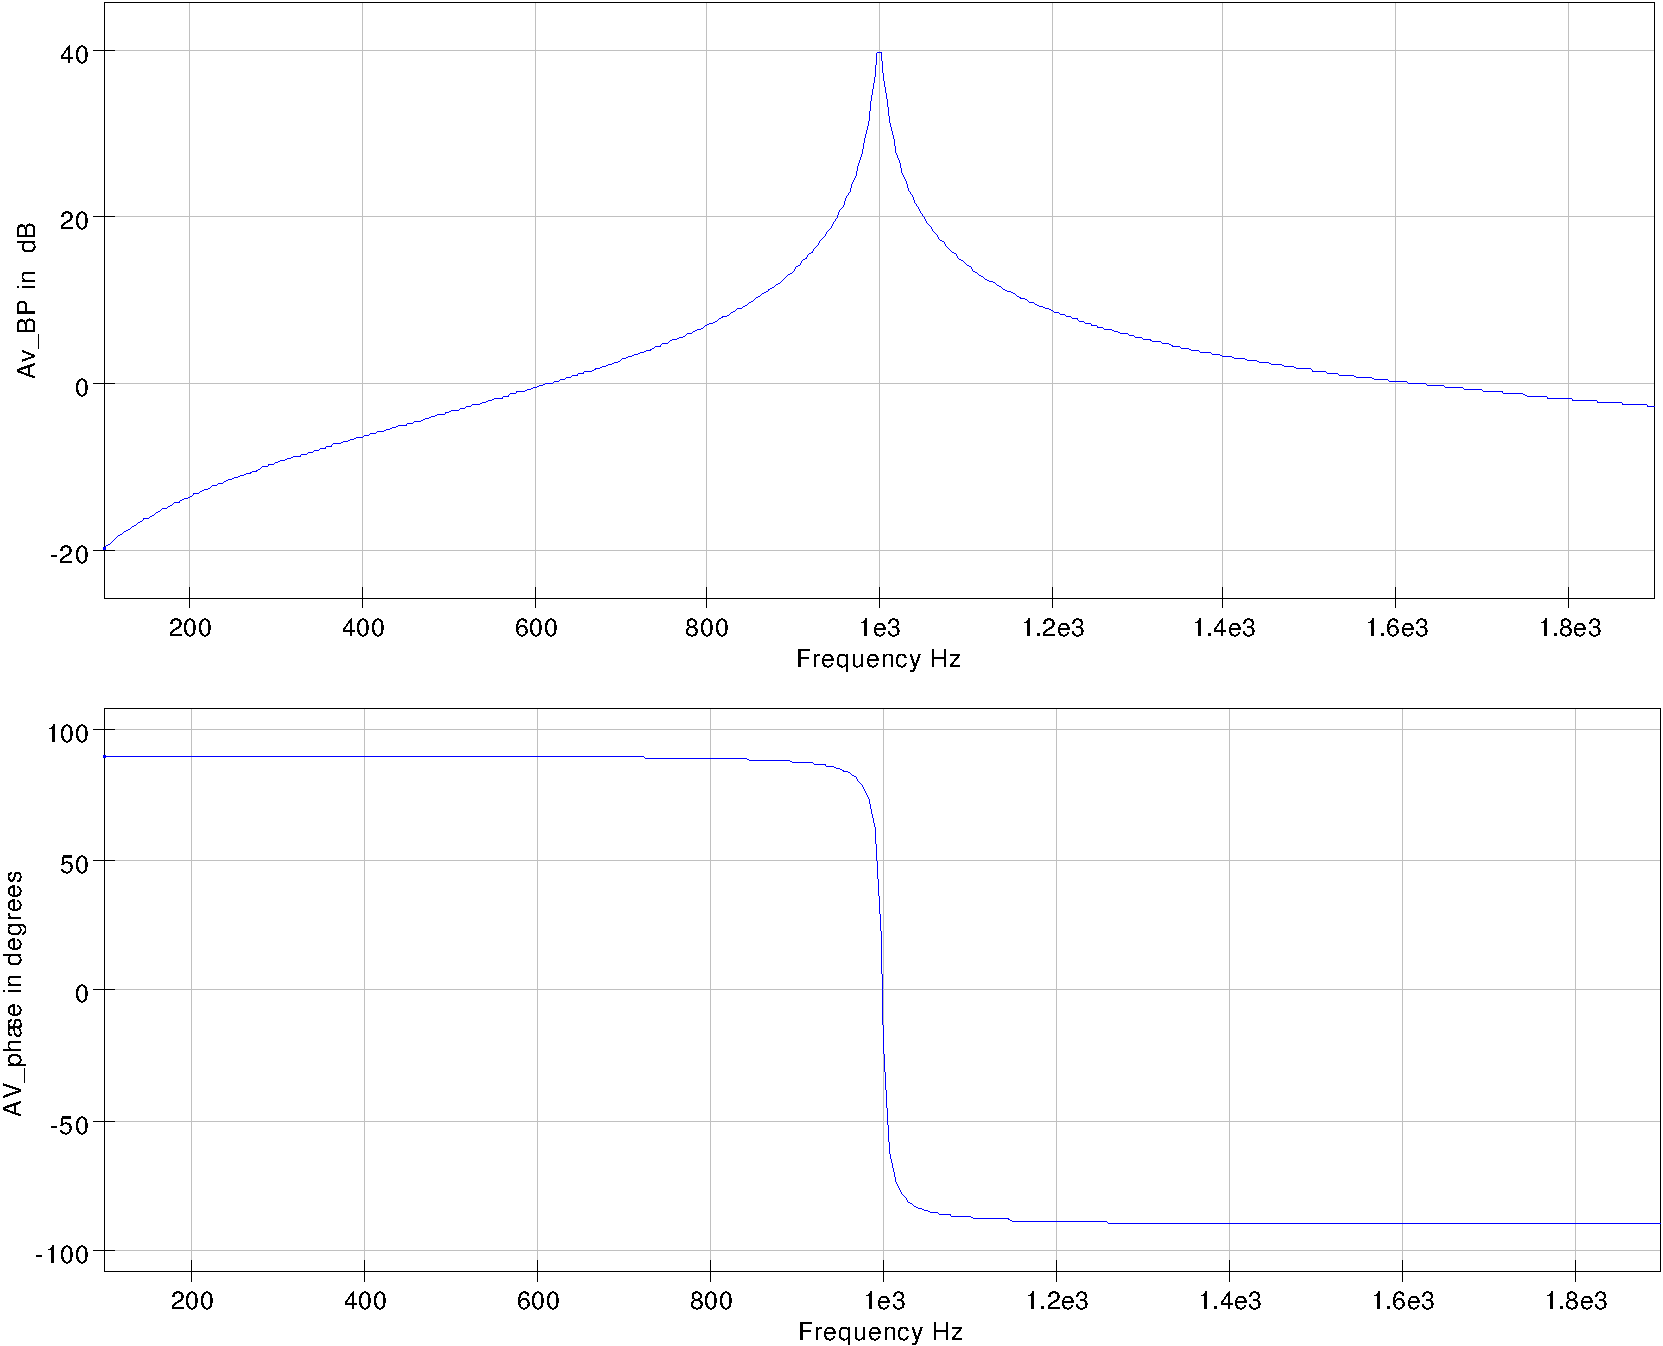
\includegraphics[width=0.9\linewidth]{fig31_dpl}
% tcomb1.png: 99.9998dpi, width=11.35cm, height=3.35cm, bb=0 0 447 132
  \caption{Simulation waveforms for current state variable filter circuit shown in Fig.~\ref{fig:opamp31}.} 
  \label{fig:opamp32}
\end{figure}

\begin{figure}
  \centering
  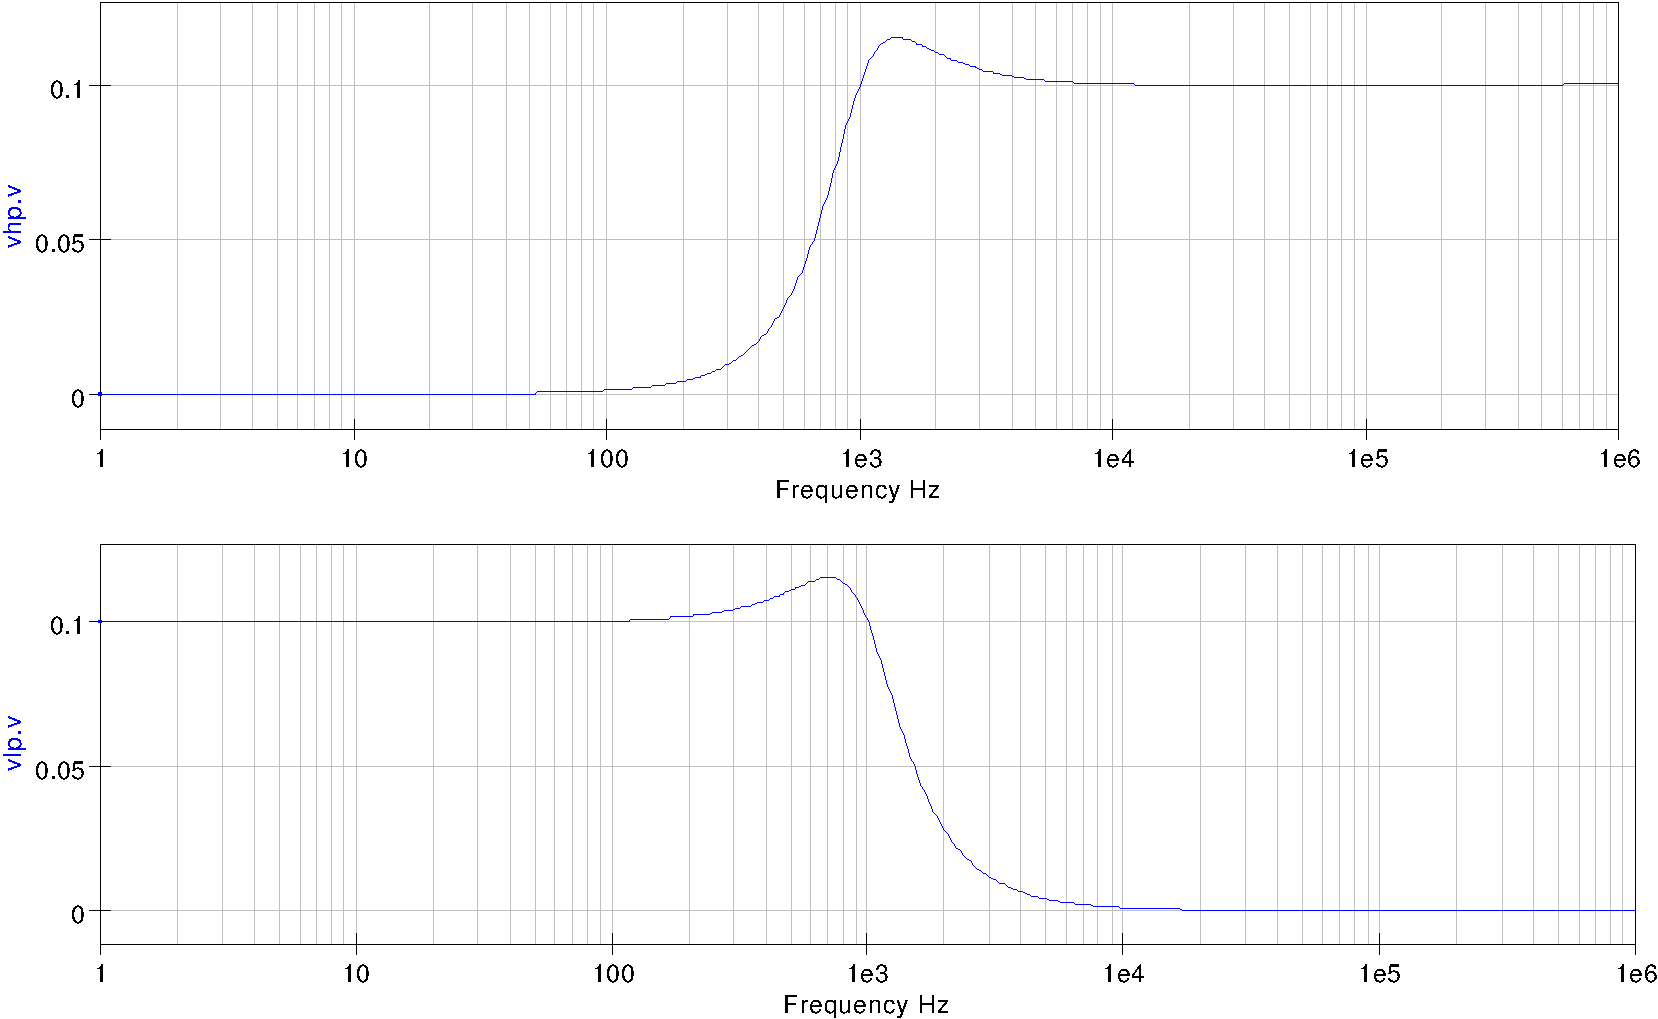
\includegraphics[width=0.9\linewidth]{fig33_dpl}
% tcomb1.png: 99.9998dpi, width=11.35cm, height=3.35cm, bb=0 0 447 132
  \caption{State variable low pass and high pass response for $Q = 1$, $R5 = 2k\Omega$.} 
  \label{fig:opamp33}
\end{figure}

\tutsubsection{Example 2: Sinusoidal signal generation with the Wien bridge oscillator} 

The Wien bridge sinusoidal oscillator has become a classic due to it's simplicity and low distortion capabilities.  It is an ideal vehicle for demonstrating the properties of OP AMP macromodels and indeed the performance of circuit simulators. Shown in Fig.~\ref{fig:opamp35} is the basic Wien bridge oscillator which consists of a single OP AMP with negative and positive feedback circuits. The design equations for this circuit are

\begin{enumerate}
\item  Non-inverting amplifier.
\begin{equation}
\dfrac{vout}{v+} = 1 + \dfrac{R3}{R4}
\end{equation}

\item Feedback factor
\begin{equation}
b = \dfrac{vout}{v+} =\dfrac{1}{3+j(\frac{f}{f_{0}}-\frac{f_{0}}{f})}
\end{equation}
Where $f_{0} = \dfrac{1}{2\pi R1 C1} =\dfrac{1}{2\pi R2 C2} $

\item Loop gain

The oscillator loop gain $b A_{v}$ must equal one for stable oscillations. Hence,
\begin{equation}
b A_{v} = \dfrac{1+\frac{R3}{R4}}{3+j(\frac{f}{f_{0}}-\frac{f_{0}}{f})}
\end{equation}

Moreover, at $f = f_{0}$,  
\begin{equation}
b A_{v} = \dfrac{1+\frac{R3}{R4}}{3}
\end{equation}

Setting $R3/R4$ slightly greater than two causes oscillations to start and increase in amplitude during each oscillatory cycle. Furthermore, if $R3/R4$ is less than two oscillations will never start or decrease to zero.
\end{enumerate}

Figure~\ref{fig:opamp36} shows a set of Wien bridge oscillator waveforms. In this example the OP AMP is modelled using the OP27 AC macromodel. This has been done deliberately to demonstrate what happens with a poor choice of OP AMP model.  The oscillator frequency is 10 kHz with both feedback capacitors and resistors having equal values. Notice that the oscillatory output voltage continues to grow with increasing time until it's value far exceeds the limit set by a practical OP AMP power supply voltages.  The lower of the two curves in Fig.~\ref{fig:opamp36} illustrates the frequency spectrum of the oscillator output signal. The data for this curve has been generated using the Time2Freq function.  Adding slew rate and voltage limiting to the OP27 macromodel will limit the oscillator output voltage excursions to the OP AMP power supply values. The waveforms for this simulation are shown in Fig.~\ref{fig:opamp37}.  When analysing transient response data using function Time2Freq it is advisable to restrict the analysis to regions of the response where the output waveform has reached a steady state otherwise the frequency spectrum will include effects due to growing, or decreasing, transients.  The voltage limiting network clips the oscillator output voltage restricting its excursions to below the OP AMP power supply voltages.  The clipping is very visible in Fig.~\ref{fig:opamp37}.  Notice also that the output waveform is distorted and is no longer a pure sinusoidal waveform of 10 kHz frequency.  Odd harmonics are clearly visible and the fundamental frequency has also decreased due to the signal saturation distortion.  In a practical Wien bridge oscillator the output waveform should be a pure sinusoid with zero or little harmonic distortion.  One way to achieve this is to change the amplitude of the OP AMP gain with changing signal level: as the output signal increases so $Av$ is decreased or as the output signal level decreases $Av$ is increased.  At all times the circuit parameters are changed to achieve the condition $b Av = 1$.  The circuit shown in Fig.~\ref{fig:opamp38} uses two diodes and a resistor to automatically change the OP AMP closed loop gain with changing signal level.  Fig.~\ref{fig:opamp39} shows the corresponding waveforms for the Wien bridge circuit with automatic gain control.  Changing the value of resistor $R5$ causes the amplitude of the oscillator output voltage to stabilise at a different value; decreasing $R5$ also decreases $vout$. The automatic gain control version of the Wien bridge oscillator also reduces the amount of harmonic distortion generated by the oscillator.  This can be clearly observed in Fig.~\ref{fig:opamp39}.  Changing the oscillator frequency can be accomplished by either changing the capacitor or resistor values in the feedback network $b$. To demonstrate how this can be done using Qucs, consider the circuit shown in Fig.~\ref{fig:opamp40}.  In this circuit time controlled switches change the value of both capacitors as the simulation progresses.  The recorded output waveform for this circuit is shown in Fig.~\ref{fig:opamp41}.


\begin{figure}
  \centering
  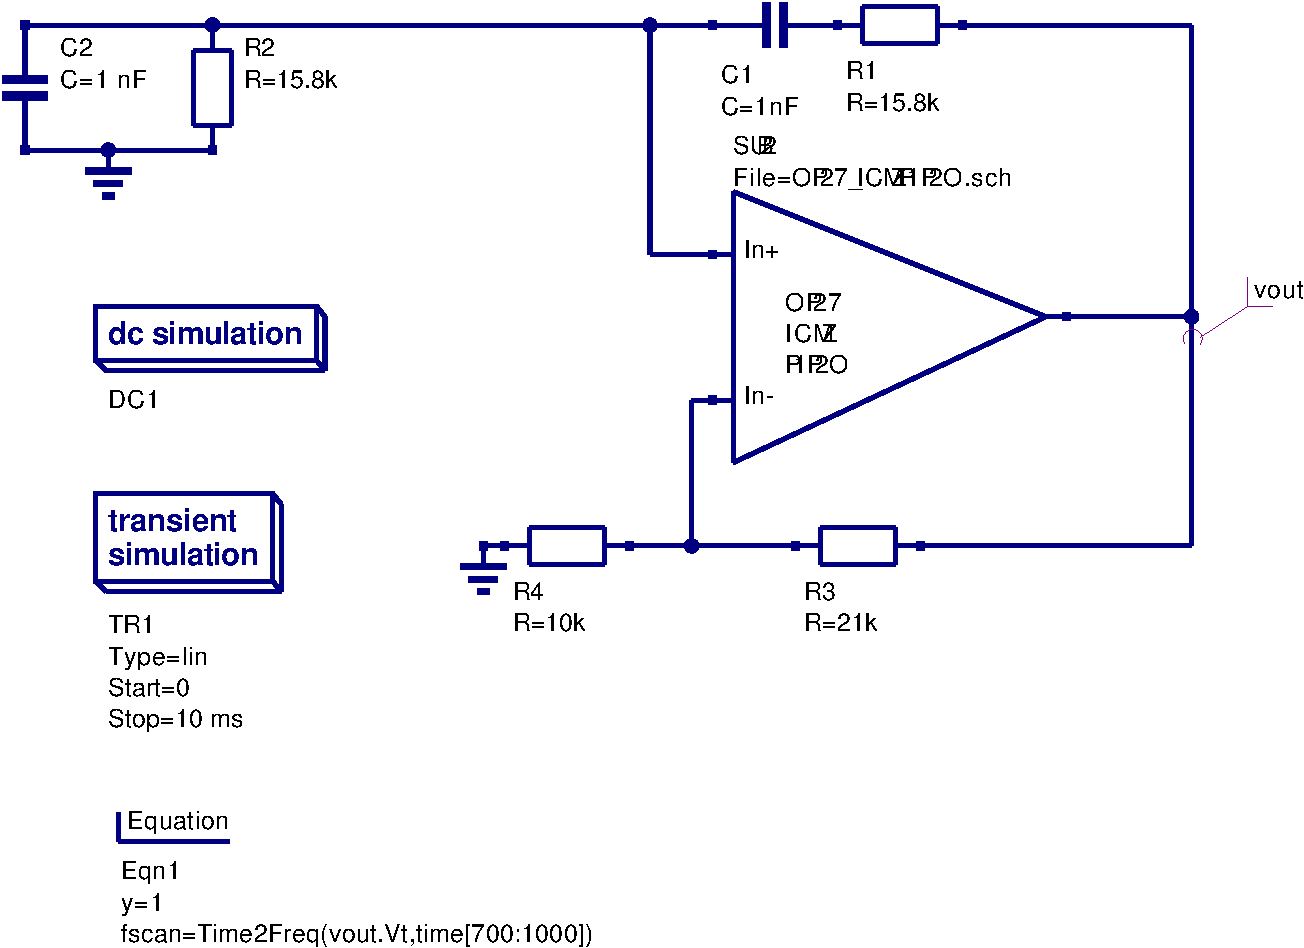
\includegraphics[width=0.9\linewidth]{fig34_sch}
% tcomb1.png: 99.9998dpi, width=11.35cm, height=3.35cm, bb=0 0 447 132
  \caption{Classic Wien bridge sinusoidal oscillator.} 
  \label{fig:opamp35}
\end{figure}

\begin{figure}
  \centering
  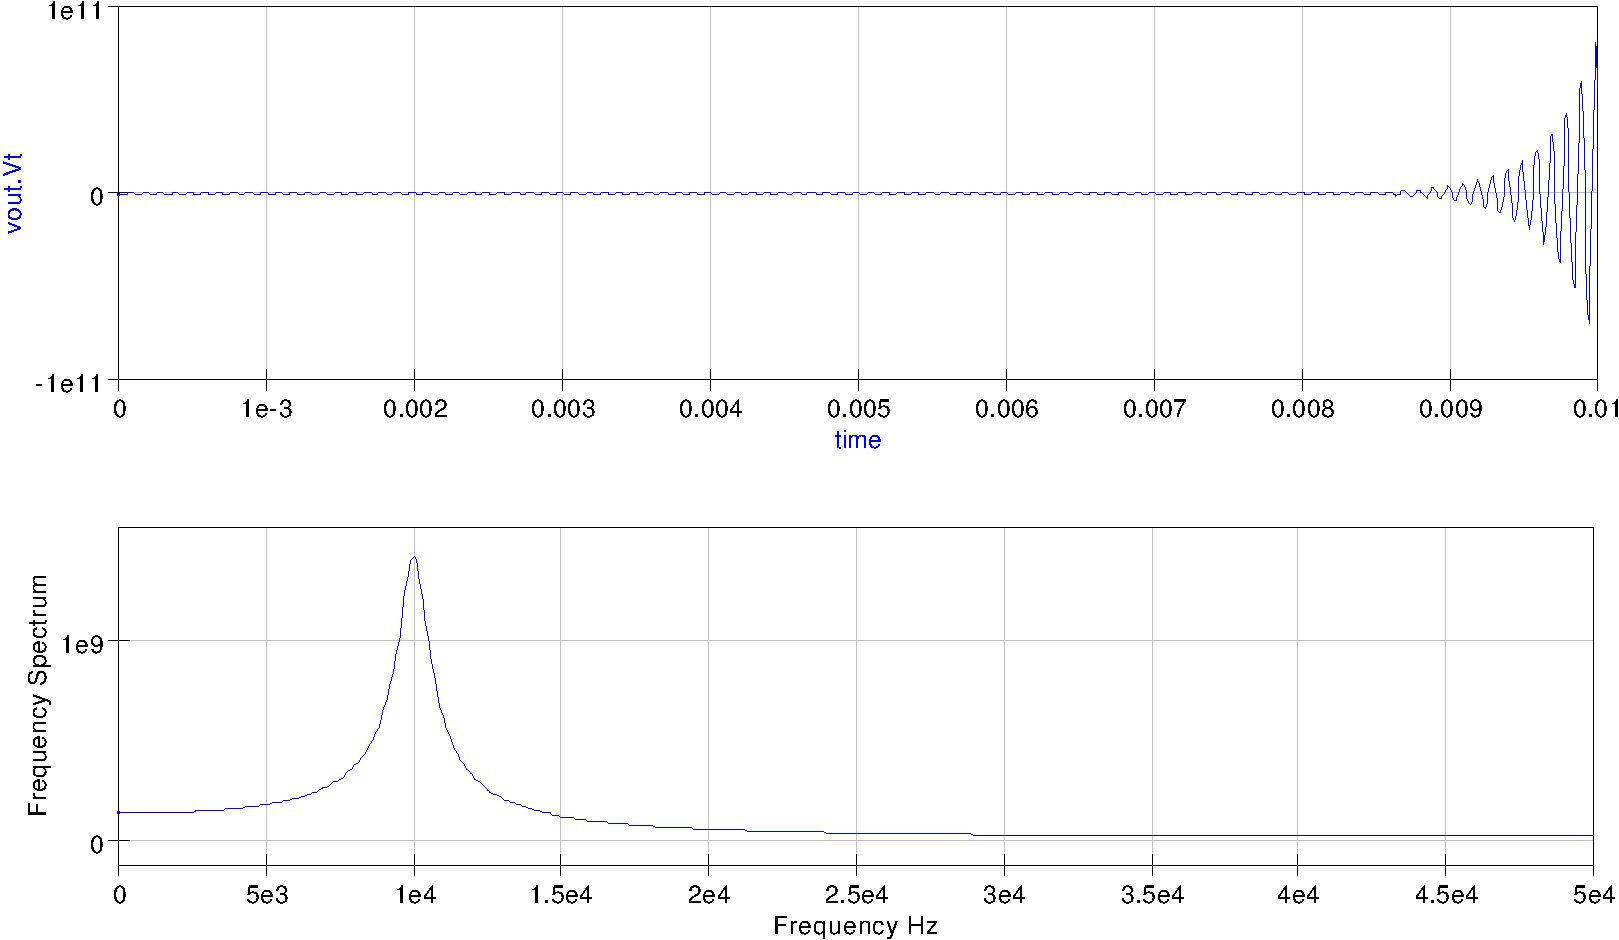
\includegraphics[width=0.9\linewidth]{fig34_dpl}
% tcomb1.png: 99.9998dpi, width=11.35cm, height=3.35cm, bb=0 0 447 132
  \caption{Simulation waveforms for the circuit shown in Fig.~\ref{fig:opamp35}: OP27 AC macromodel. } 
  \label{fig:opamp36}
\end{figure}

\begin{figure}
  \centering
  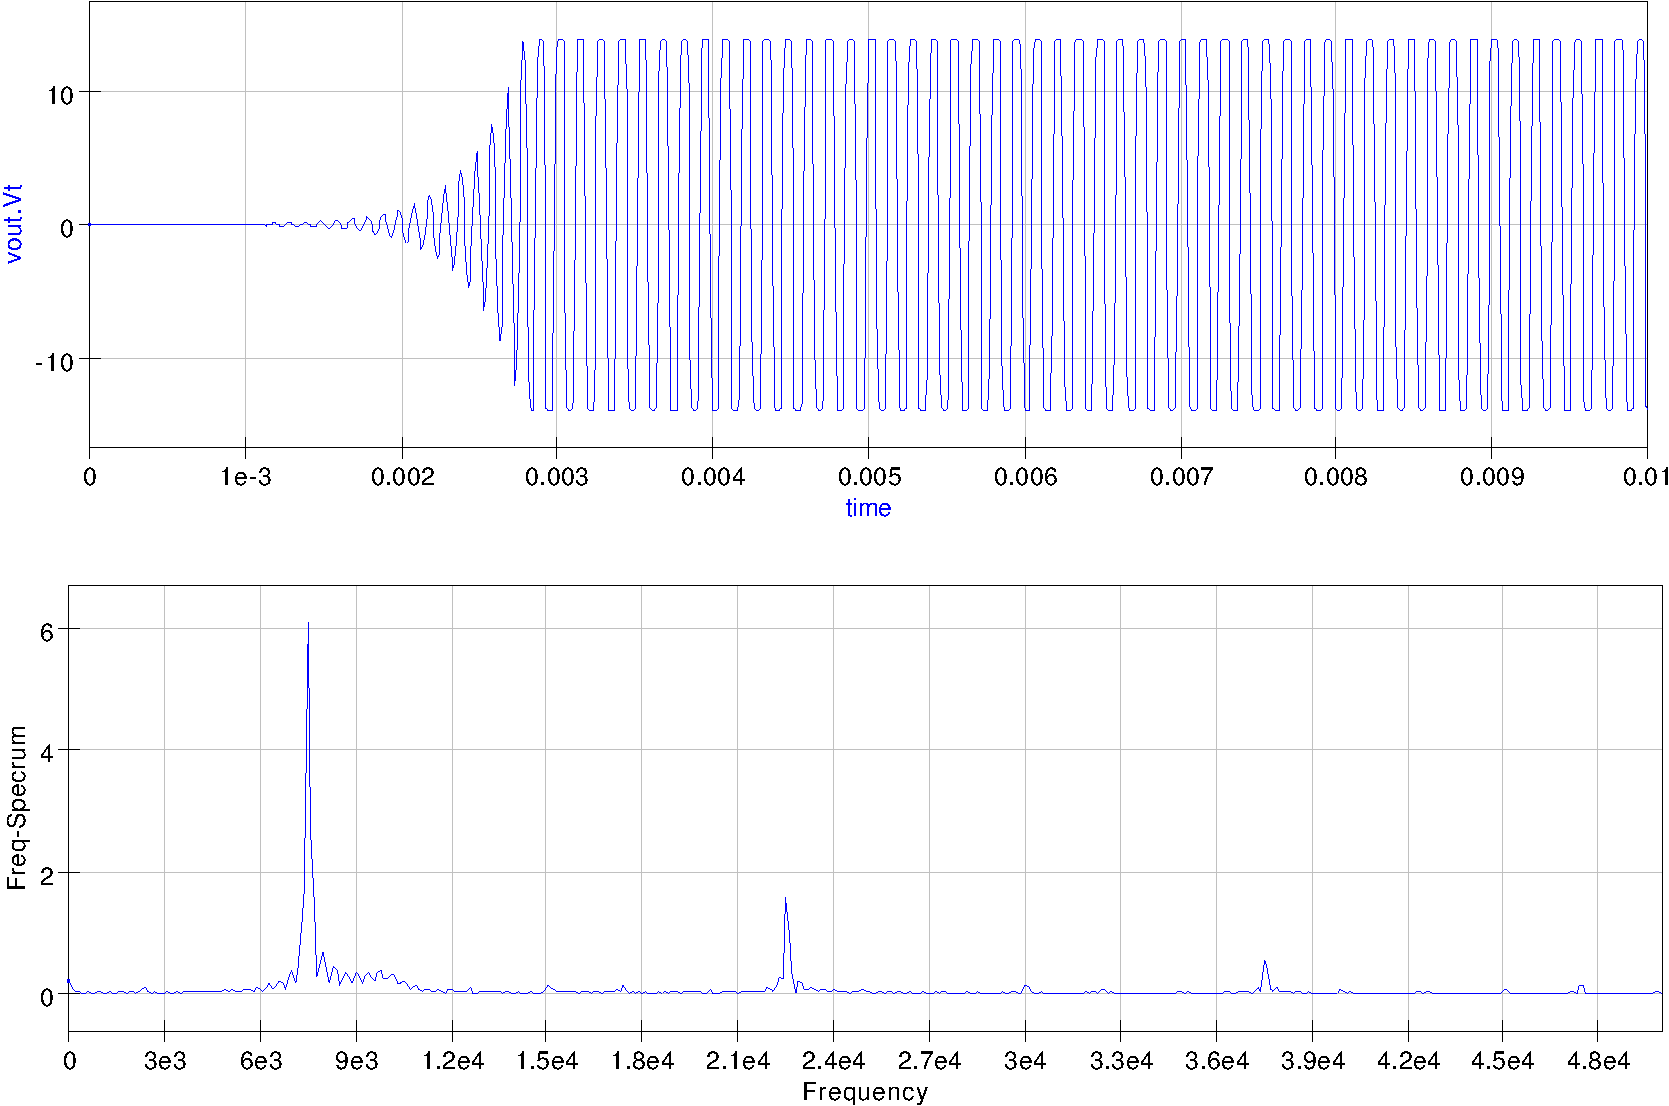
\includegraphics[width=0.9\linewidth]{fig37_dpl}
% tcomb1.png: 99.9998dpi, width=11.35cm, height=3.35cm, bb=0 0 447 132
  \caption{Simulation waveforms for the circuit shown in Fig.~\ref{fig:opamp35}: OP27 AC + slew rate + vlimit macromodel. } 
  \label{fig:opamp37}
\end{figure}

\begin{figure}
  \centering
  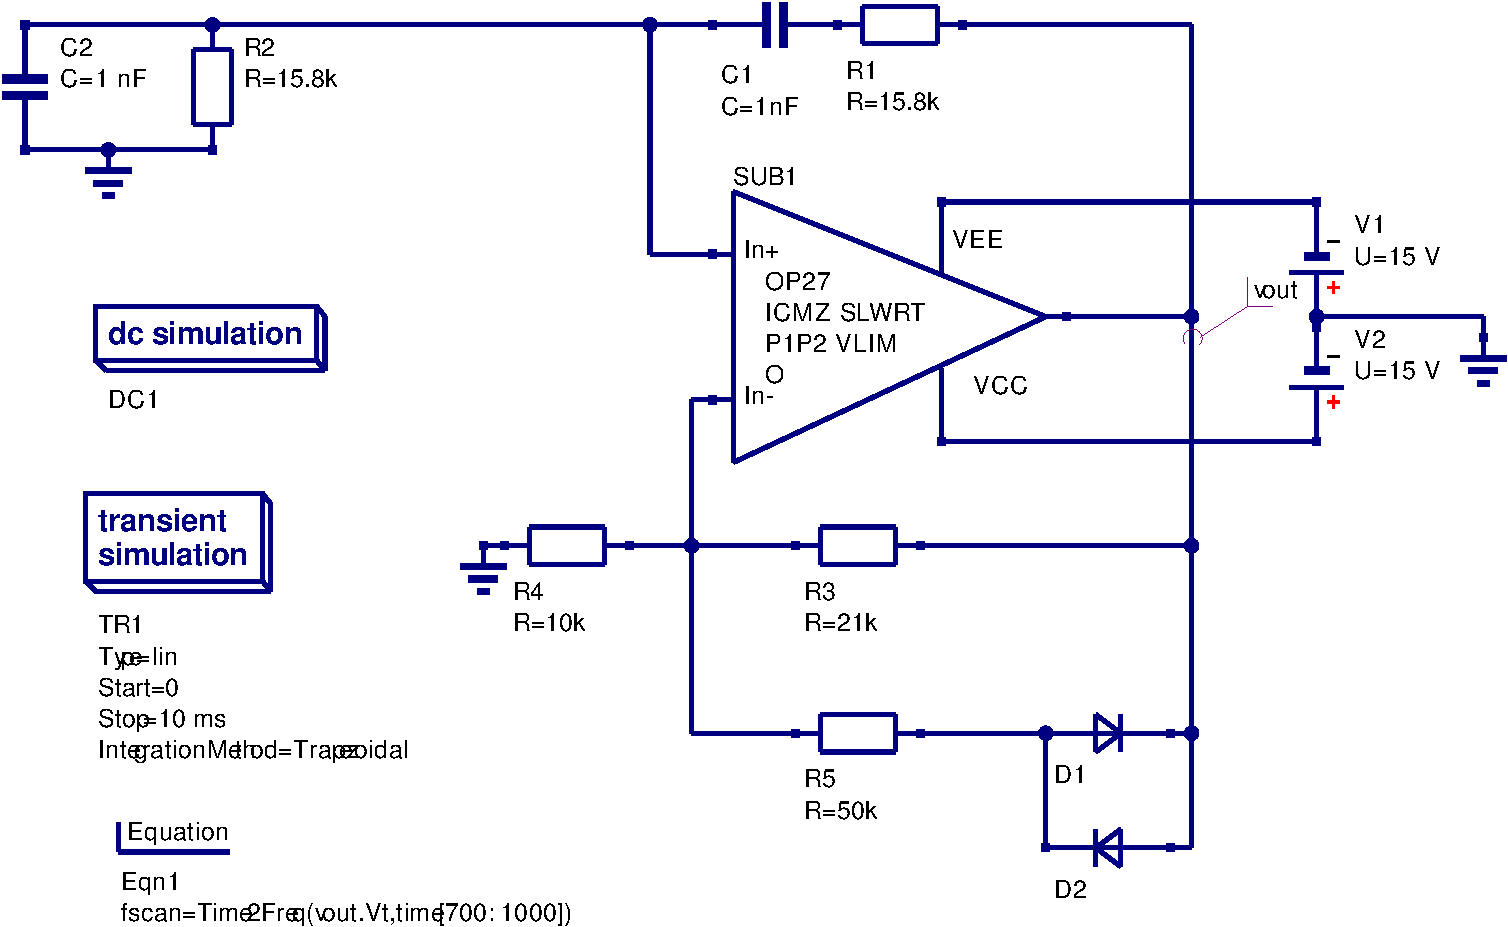
\includegraphics[width=0.9\linewidth]{fig38_sch}
% tcomb1.png: 99.9998dpi, width=11.35cm, height=3.35cm, bb=0 0 447 132
  \caption{Wien bridge oscillator with automatic gain control. } 
  \label{fig:opamp38}
\end{figure}

\begin{figure}
  \centering
  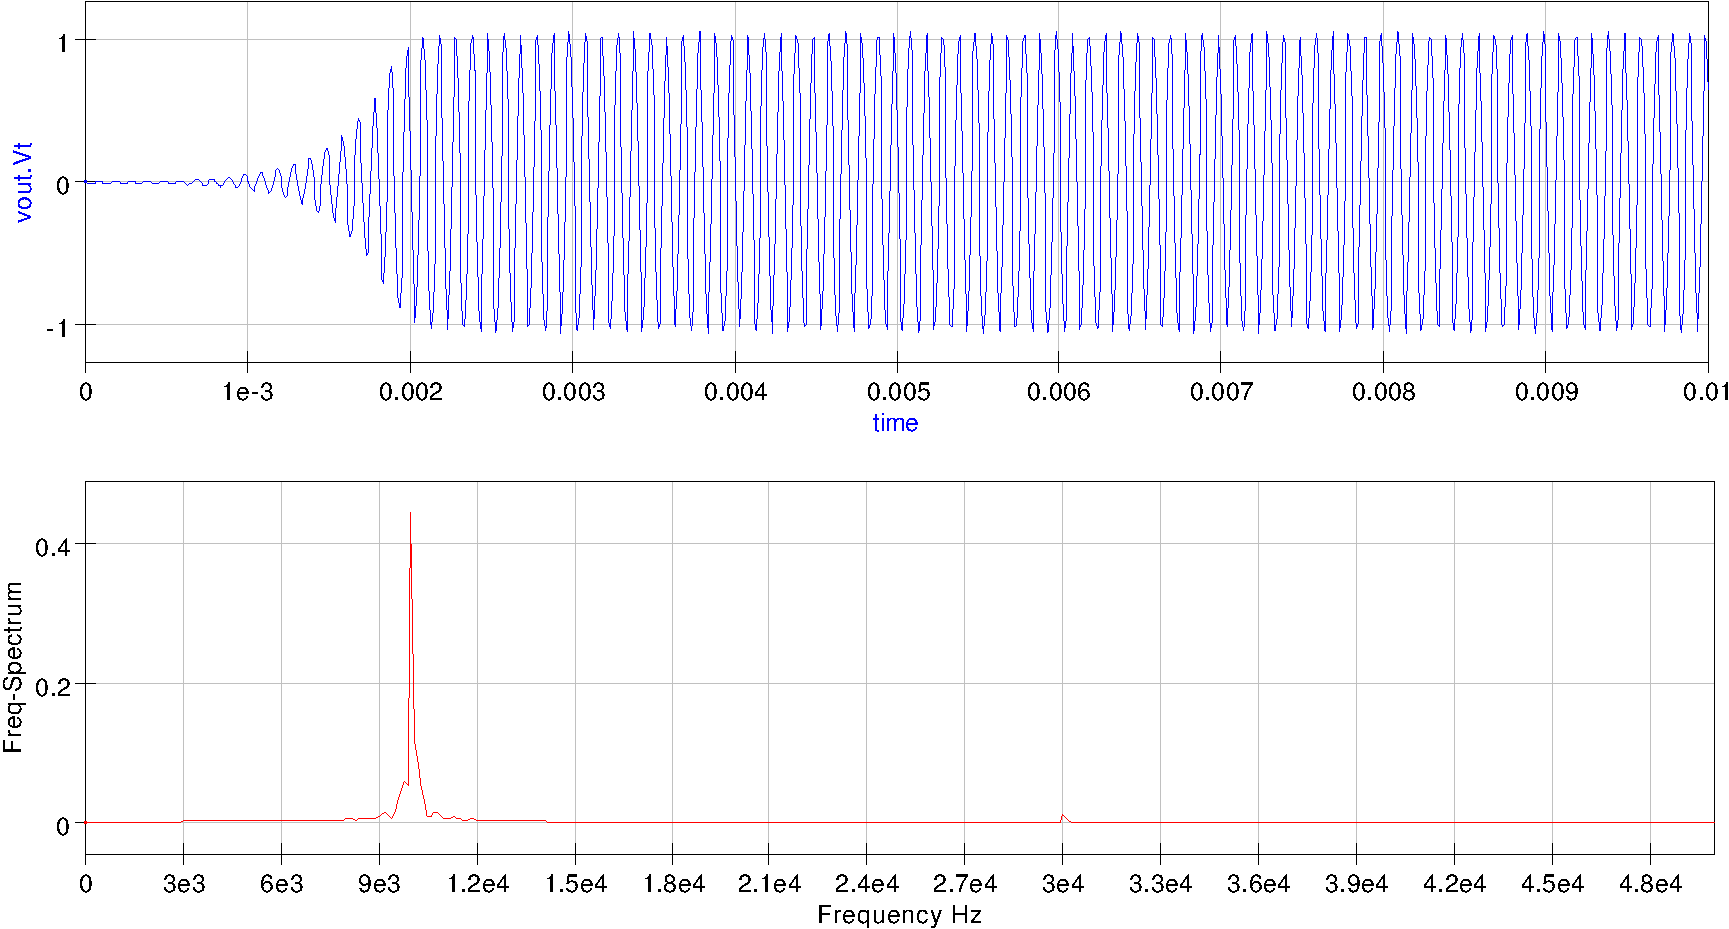
\includegraphics[width=0.9\linewidth]{fig39_dpl}
% tcomb1.png: 99.9998dpi, width=11.35cm, height=3.35cm, bb=0 0 447 132
  \caption{Simulation waveforms for the circuit shown in Fig.~\ref{fig:opamp38}: OP27 AC + slew rate + vlimit macromodel. } 
  \label{fig:opamp39}
\end{figure}

\begin{figure}
  \centering
  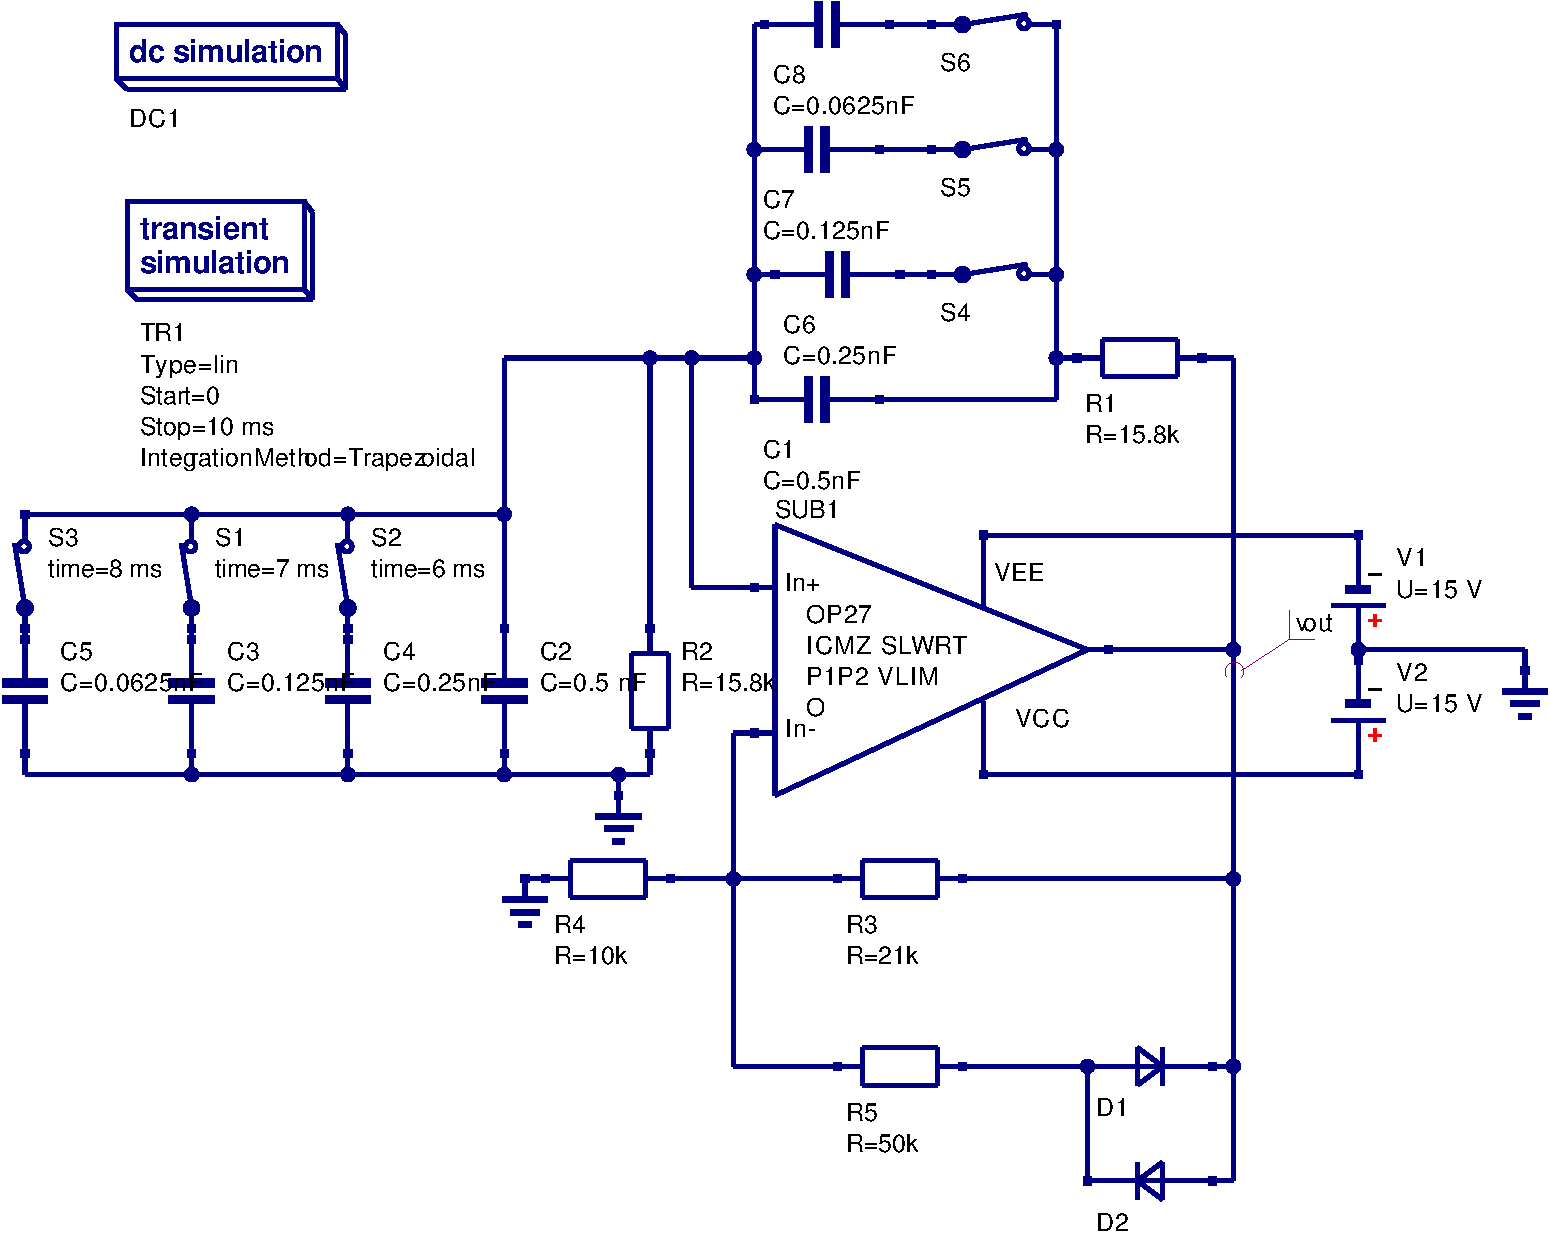
\includegraphics[width=0.9\linewidth]{fig40_sch}
  \caption{Wien bridge oscillator with switched capacitor frequency control. } 
  \label{fig:opamp40}
\end{figure}

\begin{figure} 
  \centering
  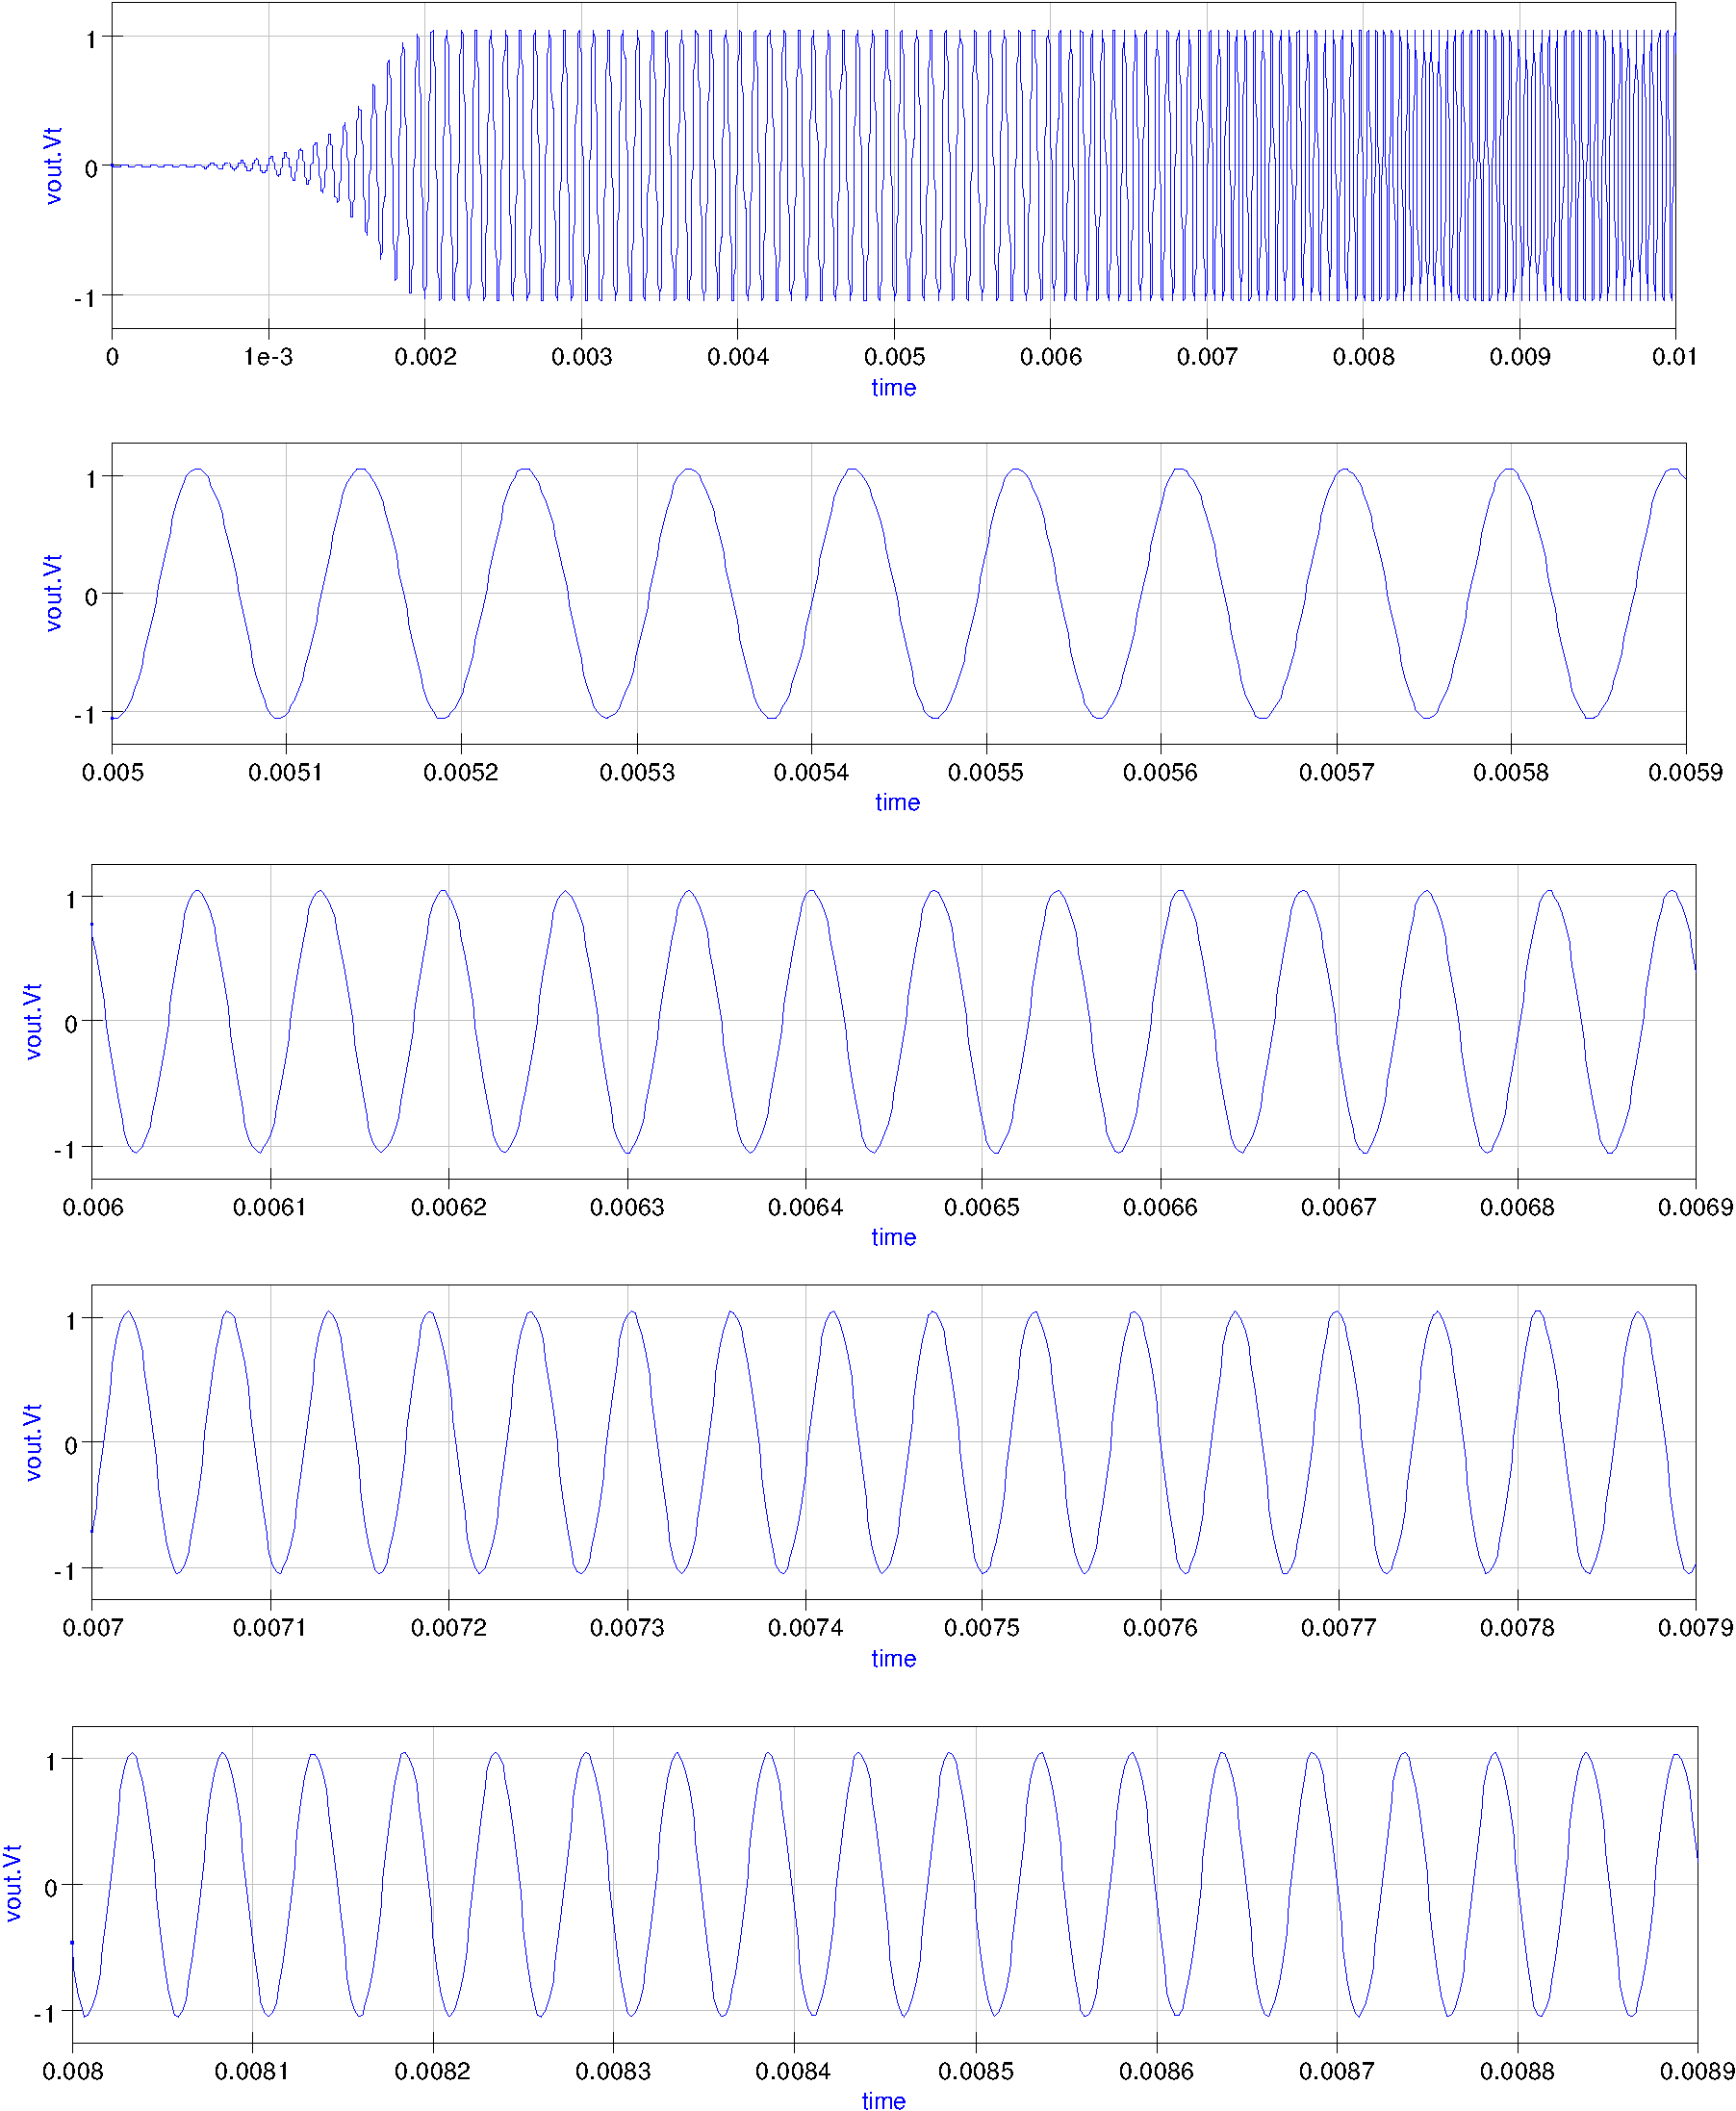
\includegraphics[width=0.9\linewidth]{fig41_dpl}
% tcomb1.png: 99.9998dpi, width=11.35cm, height=3.35cm, bb=0 0 447 132 
  \caption{Simulation waveforms for the circuit shown in Fig.~\ref{fig:opamp40}: OP27 AC + slew rate + vlimit macromodel. } 
  \label{fig:opamp41}
\end{figure}

\tutsection{End note}

While writing this tutorial I have tried to demonstrate how practical models of operational amplifiers can be constructed using basic electronic concepts and the range of Qucs built-in models included in release 0.0.9.  The modular OP AMP macromodel was deliberately chosen as the foundation for the tutorial for two reasons; firstly Qucs release 0.0.9 is mature enough to simulate such models, and secondly the parameters which determine the operation of the macromodel can be easily be calculated from information provided on device data sheets. This tutorial must be considered very much as work in progress because a number of significant OP AMP properties are not included in the macromodel described in previous sections. These, for example, include power supply rejection and noise properties. In the future, if other Qucs users find these notes helpful and indeed if the response to them is positive, I will update the OP AMP modelling tutorial.  Other significant sections will also need to be added once the non-linear controlled source models from Stefan's to-do list have been added to Qucs. It will then be possible to expand the range of macromodels that Qucs can simulate to include the Boyle model and the more advanced variations that are often provided by device manufacturer's data sheets.  My thanks to Dr David Faulkner\footnote{Department of Computing, Communications Technology and Mathematical Science, London Metropolitan University, UK.} for all his help and support during the period we were working on many of the concepts that form the basis of this tutorial. Once again a special thanks to Michael Margraf and Stefan Jahn for all their help and encouragement over the period that I have been writing this tutorial and testing the many examples it includes.